%% ============================================================================
%% UCL Mechanical Engineering — MSc Thesis Template (Journal Article Format)
%% Programme: MSc Engineering with Finance (MECH0085)
%% ============================================================================
%% Formatting per: MSc Thesis Writing Guidance 2025-26 V0.0
%%   - A4, moderate margins (top/bottom 2.54cm, left/right 1.91cm)
%%   - Times New Roman 11pt, single spacing, first-line indent 0.25cm
%%   - IEEE referencing style
%%   - 15–20 pages max (excl. cover sheet & references), appendix ≤5 pages
%% ============================================================================

\documentclass[11pt, a4paper]{article}

%% ── Page geometry (UCL "moderate" margins) ──────────────────────────────────
\usepackage[
  top=2.54cm,
  bottom=2.54cm,
  left=1.91cm,
  right=1.91cm
]{geometry}

%% ── Font: Times New Roman ───────────────────────────────────────────────────
%% (Use newtxtext + newtxmath for a complete Times-compatible setup in LaTeX)
%% If you prefer Arial, replace with: \usepackage{helvet}\renewcommand{\familydefault}{\sfdefault}
\usepackage{newtxtext}
\usepackage{newtxmath}
\usepackage{mathtools}
\usepackage[T1]{fontenc}
\usepackage[utf8]{inputenc}

%% ── Spacing: single line spacing, 0.25cm first-line indent ─────────────────
\usepackage{setspace}
\singlespacing
\setlength{\parindent}{0.25cm}

%% ── Core packages ───────────────────────────────────────────────────────────
\usepackage{amsmath, amssymb, amsthm}      % Mathematics
\usepackage{graphicx}                       % Figures
\usepackage{subcaption}                     % Subfigures: (a), (b), (c)
\usepackage{booktabs} 
\usepackage{threeparttable}% Professional tables
\usepackage{multirow}
\usepackage{longtable}                       % Nomenclature (page-breaking, non-float)
\usepackage{siunitx}                        % SI units (required by guidance)
\usepackage[ruled, vlined]{algorithm2e}     % Algorithms (numbered, ruled)
\usepackage{hyperref}                       % Clickable cross-references
\usepackage{cleveref}                       % Smart referencing (\cref)
\usepackage{xcolor}                         % Colour (for draft annotations)
\usepackage{enumitem}                       % List formatting
\usepackage{float}                          % Figure placement control
\usepackage{caption}   
\usepackage{tikz}% Caption formatting
\usepackage{xcolor}
\usetikzlibrary{positioning,arrows.meta,fit,backgrounds,calc}


%% ── Custom title block (thick rules + small caps, conference style) ──────
\newcommand{\thesistitle}{%
  \vspace*{0.2cm}%
  \noindent\rule{\textwidth}{1.5pt}%
  \vspace{0.6cm}%
  \begin{center}%
    {\Large\scshape AP-PEN: A Hard-Constrained, Physics-Enforced Network for Convenience-Yield Inversion from Commodity Futures — A WamOL Approach}%
  \end{center}%
  \vspace{0.4cm}%
  \noindent\rule{\textwidth}{1.5pt}%
  \vspace{0.8cm}%
  \begin{center}%
    \textbf{Evan Lynch}\\[4pt]
    Department of Mechanical Engineering\\[2pt]
    University College London\\[2pt]
    \texttt{[evan.lynch.25]@ucl.ac.uk}%
  \end{center}%
  \vspace{0.6cm}%
}

%% ── Headers and footers ────────────────────────────────────────────────────
\usepackage{fancyhdr}
\pagestyle{fancy}
\fancyhf{}  % Clear all
\fancyhead[L]{\small\textit{UCL Mechanical Engineering}}
\fancyhead[R]{\small\textit{AY\,2025--26}}
\fancyfoot[C]{\small\thepage}
\renewcommand{\headrulewidth}{0.4pt}
\renewcommand{\footrulewidth}{0pt}
%% Also apply to plain pages (first page of sections):
\fancypagestyle{plain}{%
  \fancyhf{}
  \fancyhead[L]{\small\textit{MSc Engineering with Finance: UCL Mechanical Engineering}}
  \fancyhead[R]{\small\textit{2025--26}}
  \fancyfoot[C]{\small\thepage}
  \renewcommand{\headrulewidth}{0.4pt}
}

%% ── PDF inclusion (for cover sheet) ───────────────────────────────────────
\usepackage{pdfpages}

%% ── Hyperlink styling ──────────────────────────────────────────────────────
\hypersetup{
  colorlinks=true,
  linkcolor=black,
  citecolor=blue!60!black,
  urlcolor=blue!60!black,
}

%% ── Caption formatting (guidance: full sentences, below figures) ────────────
\captionsetup{
  font=small,
  labelfont=bf,
  labelsep=period,
  justification=justified,
  singlelinecheck=false,
}
%% Use "Fig." for figures (per guidance: use "Fig." even at start of sentence)
\captionsetup[figure]{name=Fig.}

%% ── IEEE-style referencing ──────────────────────────────────────────────────
%% Requires: IEEEtran.bst in your Overleaf project (upload it, or use the
%% package below which is available on most TeX distributions)
\usepackage{cite}  % Sorts and compresses [1]-[3] style citations

%% ── Draft helper: comment command (remove before submission) ────────────────
\newcommand{\todo}[1]{\textcolor{red}{\textbf{[TODO: #1]}}}
\newcommand{\note}[1]{\textcolor{blue}{\textbf{[NOTE: #1]}}}
%% To hide all TODOs for final submission, uncomment:
% \renewcommand{\todo}[1]{}
% \renewcommand{\note}[1]{}

%% ── Custom math shortcuts for this project ──────────────────────────────────
\DeclareMathOperator{\E}{\mathbb{E}}        % Expectation
\newcommand{\R}{\mathbb{R}}                  % Real numbers
\newcommand{\bx}{\mathbf{x}}                % Bold x (input vector)
\newcommand{\btheta}{\boldsymbol{\theta}}    % Network parameters
\newcommand{\Lhat}{\widehat{\mathcal{L}}}   % WamOL loss
\newcommand{\convyield}{\delta}             % Convenience yield symbol
\newcommand{\meanrev}{\kappa}               % Mean-reversion speed
\newcommand{\longrun}{\alpha}               % Long-run convenience yield


%% ============================================================================
%% DOCUMENT BEGINS
%% ============================================================================
\begin{document}

%% ── PAGE BUDGET (body only; 20-page limit) ──────────────────────────────────
%%   Abstract + title                        0.5
%%   1. Introduction                         1.5
%%   2. Literature Review                    3.0   (was ~4; compress 2.1-2.2)
%%   3. Methodology                          5.5   (was ~7; merges above)
%%   4. Results                              5.5   (was ~1; the growth area)
%%   5. Discussion                           2.5
%%   6. Conclusion                           0.75
%%                                          -----
%%                                          19.25
%% Results and Discussion together should be ~40% of the body. They are
%% currently ~15%. Every page freed in Methodology goes to Section 4.
%% Going over the limit is a flat 10-percentage-point deduction.

%% ── COVER SHEET ─────────────────────────────────────────────────────────────
%% Import the cover sheet (does NOT count toward 20-page limit).
%% Compile cover_sheet.tex separately first, then include the PDF here:
% \includepdf[pages=-]{cover_sheet.pdf}


%% ── TITLE BLOCK ─────────────────────────────────────────────────────────────
%% Conference/journal style: thick rules + small caps title + author block.

\thesistitle
\thispagestyle{fancy}  % Keep header on title page


%% ════════════════════════════════════════════════════════════════════════════
%% ABSTRACT
%% ════════════════════════════════════════════════════════════════════════════
%% Guidance: Single paragraph, ≤300 words. Stand-alone reflection of contents.
%% Must contain: brief intro, work reported, main conclusions.
%% Must NOT contain: displayed equations, references, footnotes.

\begin{abstract}
Commodity futures prices depend on the convenience yield, the implicit benefit
of holding physical inventory, which is latent and must be inferred from the
observed term structure. The incumbent approach casts the Gibson--Schwartz
two-factor model in state space and applies a Kalman filter, which is
linear-Gaussian by construction and cannot accommodate economic inequality
constraints. This thesis develops the Affine-Partitioned, Physics-Enforced
Network, which separates the model's closed-form futures price into a
deterministic affine term-structure map, imposed analytically, and the latent
convenience-yield path, parameterised by a single neural network. Because that
affine map satisfies the pricing partial differential equation identically for
any convenience yield, the physics is enforced by construction rather than
penalised, and no differential-equation residual remains in the objective;
what remains is a data-misfit term, a physical-measure transition likelihood,
and no-arbitrage inequality penalties balanced by a gradient-norm scheme. A
structural identifiability result frames the evaluation: the futures
cross-section determines only three combinations of the five risk-neutral
parameters, so spot volatility, Brownian correlation and the risk-neutral
long-run level are individually non-estimable from prices by any method. On
simulated panels with known ground truth the network recovers the latent path
robustly across independent draws and under tenfold observation noise, and recovers the identified combinations to within a few per cent while
the unidentified ones vary by an order of magnitude more. Two controls temper
this. A closed-form per-date least-squares inversion, requiring no training,
recovers the path more accurately and reproduces the high-frequency variation
the network oversmooths. On real WTI data the network, that least-squares
solution and the filter disagree systematically, with the two cross-sectional
estimators closely agreeing; the constrained variant matches the filter most
closely, but only by converging onto its own constraint boundaries. The
contribution is an identification analysis and a constrained
latent-path estimator, benchmarked against both incumbents.
\end{abstract}


%% ── KEYWORDS ────────────────────────────────────────────────────────────────
\vspace{0.3cm}
\noindent\textbf{Keywords:} Physics-Informed Neural Networks, Whack-a-mole Online Learning,
Convenience Yield, Gibson--Schwartz Model, Commodity Futures, Latent State Estimation,
Multi-Objective Optimisation


%% ════════════════════════════════════════════════════════════════════════════
%% 1. INTRODUCTION
%% ════════════════════════════════════════════════════════════════════════════
%% Guidance: Background of topic and problem. Start at general engineering
%% level, then narrow. Must be accessible to non-specialists initially.
%% ~1.5–2 pages.

\section{Introduction}
\label{sec:introduction}

Commodities such as crude oil are primarily traded via futures contracts: standardised agreements to buy or sell a fixed quantity of the underlying asset at a predetermined price on a set future date. These contracts allow speculators and hedgers to take positions on future price movements, and the resulting market activity makes futures prices a key mechanism for price discovery, aggregating participants' collective expectations of supply and demand. In crude oil markets specifically, the relationship between spot and futures prices is further shaped by the cost and benefit of physical storage, captured in the concept of convenience yield: the implicit return accruing to holders of the physical commodity rather than a futures contract. Estimating this variable is vital for risk management, hedging and procurement. This thesis focuses on WTI crude oil, the most widely benchmarked and liquid contract in the global oil market, as the setting for this estimation problem.

Accurate estimation in practice is difficult: convenience yield is, by nature, a \textit{latent} state and is not directly observable. Traditional approaches employ Kalman filters to reconstitute and track hidden state variables in commodity pricing models~\cite{Schwartz1997TheHedging}. While highly useful, these assume linearity and Gaussian noise, ignoring the Partial Differential Equation (PDE) and no-arbitrage constraints inherent to the model.

Physics-informed neural networks (PINNs), an architecture within the broader unsupervised learning paradigm, are a comparatively recent development. While they have been widely applied across engineering and physics, embedding governing differential equations directly into the learning process, their adoption in financial computing has emerged only recently. Whack-a-Mole Online-Learning (WamOL) is one such example, integrating self-adaptive weights and online learning into the PINN framework. This thesis extends the work of Hoshisashi et al.~\cite{Hoshisashi2024Whack-a-moleSurface}, adapting WamOL to commodity markets to estimate the instantaneous convenience yield in the Gibson–Schwartz (GS) two-factor model. What carries over from WamOL is the gradient-norm loss balancer and the derivative-constrained inequality-penalty mechanism (Section~\ref{sec:lit_pinns}); the PDE-residual loss term does not, since the exact affine imposition at the centre of AP-PEN (Section~\ref{sec:pinn_inversion}) satisfies the pricing PDE by construction and leaves no residual to penalise.
This thesis therefore asks whether AP-PEN, a hard-constrained neural inversion of this kind, can recover convenience yield from observed futures term structure with comparable or superior accuracy to Kalman filter-based methods, while respecting the no-arbitrage structure of the Gibson–Schwartz PDE. The main contributions of this thesis are summarised as follows:

\begin{itemize}
    \item \textbf{An affine-partitioned architecture for latent-state inversion:} separation of the Gibson--Schwartz closed form into a deterministic affine term-structure map, $A(\tau)$ and $B(\tau)$, imposed analytically at every step, and a single network parameterising the latent convenience-yield path $\hat{\delta}_\phi(t)$. Because the affine map solves the pricing PDE identically for any $\delta$, the constraint is satisfied by construction rather than penalised: the architecture contains no PDE-residual loss term, and the physics enters as a hard structural constraint alongside a $\mathbb{P}$-measure transition likelihood and inequality penalties.
    \item \textbf{An identifiability analysis of the Gibson--Schwartz futures cross-section:} a proof that a futures panel determines only three combinations of the five risk-neutral parameters, $(\kappa, \sigma_2, m)$ with $m = \alpha^{\mathbb{Q}} + \rho\sigma_1\sigma_2/\kappa$, so that $\sigma_1$, $\rho$ and $\alpha^{\mathbb{Q}}$ are individually non-identifiable from prices by any estimator (Section~\ref{sec:identifiability}). This bounds the incumbent method as well as the proposed one, and reframes what an inversion of this kind can be asked to deliver.
    \item \textbf{Identification and encoding of commodity-specific constraints:} formulation of model-free economic inequality constraints specific to physical commodity markets. All constraints entering the objective are of this kind, evaluated on observed $(S_t, \tau, r_t)$ and the recovered path alone; no model-based derivative constraint is claimed or implemented.
    \item \textbf{Validation on synthetic and real commodity futures data:} evaluation on Monte Carlo–simulated data generated using the Schwartz~\cite{Schwartz1997TheHedging} parameterisation, and on real futures data from Refinitiv.
    \item \textbf{Benchmarking against Kalman filter estimation:} comparison of the final AP-PEN architecture and predictions against a Kalman filter baseline fitted by maximum likelihood on the same WTI panel.
\end{itemize}


% --- 1.3 Recent advances: PINNs and WamOL ---
% Physics-informed neural networks embed governing PDEs into the learning
% process. WamOL (Hoshisashi et al., 2024) extended PINNs with self-adaptive
% weights, loss balancing, and online learning for real-time IVS calibration
% in equity markets. The framework explicitly identifies extension to other
% PDE-constrained domains as future work.

% --- 1.4 This work: contribution statement ---
% This paper adapts WamOL to estimate the latent convenience yield in the
% Gibson–Schwartz two-factor commodity model. The key contributions are:
% (a) formulation of the GS futures PDE within the WamOL loss architecture,
% (b) identification and encoding of commodity-specific constraints,
% (c) validation on synthetic and real commodity futures data,
% (d) benchmarking against Kalman filter estimation.

% --- 1.5 EF programme alignment ---
% Briefly state: engineering contribution (PINN architecture, PDE-constrained
% optimisation, state estimation) and finance contribution (commodity pricing
% theory, no-arbitrage, convenience yield economics).

% --- 1.6 Paper structure ---
% "The remainder of this article is organised as follows: Section 2..."

\section{Literature Review}
\label{sec:literature}

\subsection{Commodity Futures and the Convenience Yield}
\label{sec:fin_fun}
\label{sec:lit_commodity_merged}
% Compressed from ~a page of efficient-markets and microstructure background to
% the single paragraph below: only the arbitrage-discipline argument bears on
% the inverse problem, since it is what licenses the no-arbitrage inequality
% constraints of Section~\ref{sec:constraints}. All original citations retained.

Financial economics is grounded in the concept of \textit{market efficiency}: under Fama's Efficient Market Hypothesis, prices already incorporate historical, public and private information, so investors cannot consistently outperform the market average~\cite{Fama1970EfficientWork, ShivakumarGT.2018TheEfficieny}. Real markets deviate from this ideal, most importantly through \textit{information asymmetry}, and market microstructure relaxes several of Fama's assumptions to study how prices actually form~\cite{ShivakumarGT.2018TheEfficieny, deJong2009Introduction}. What microstructure does \emph{not} relax, and what matters for the inverse problem posed here, is the discipline imposed by arbitrage: even in informationally imperfect markets, prices across related instruments are held together because any deviation permitting a riskless profit is quickly traded away. This principle underpins the derivatives market~\cite{Hull2022OptionsDerivatives}, and it is what licenses treating the cash-and-carry inequalities of Section~\ref{sec:constraints} as constraints the recovered path must respect rather than as merely conventional bounds.

Futures contracts are exchange-traded, standardised agreements to buy or sell a specified asset at a designated future date and price. Their pricing is a direct application of arbitrage-free logic through the cost-of-carry model~\cite{Hull2022OptionsDerivatives}. An investor can secure an asset at a future date in two economically equivalent ways: enter into a futures contract today, or borrow at the risk-free rate, buy the asset at the current \textit{spot} price, and hold it until the future date~\cite{Hull2022OptionsDerivatives}. Because both strategies deliver the same asset at the same date, no-arbitrage requires them to cost the same, giving the relationship between a futures price $F$ and a spot price $S$:

\begin{align} \label{eq:futures_simple}
F = Se^{r(T-t)},
\end{align}

where $r$ is the risk-free rate and $(T-t)$ is the time-to-maturity.

While elegant, this model cannot price physical commodities, because it ignores the cost of storage and the effects of consumption. Holding a barrel of oil is not the same as holding a share of stock: it incurs real storage costs, but it also confers a benefit that a purely financial asset does not, namely immediate access to a physical good that may be needed on short notice~\cite{Hull2022OptionsDerivatives}. The need for this benefit is revealed by a contradiction between classical storage theory and observed market behaviour. Under the classical view, the cost of carrying inventory is always positive, so the futures price should always exceed the spot price, a condition known as \textit{contango}. In practice, markets frequently exhibit the opposite pattern, \textit{backwardation}, introduced by Keynes~\cite{Keynes1930AMoney} in which the spot price exceeds the futures price. To reconcile theory with this observation, Kaldor, Working, and Brennan~\cite{Kaldor1939Source:Studies, Working1949TheStorage, Brennan1958TheStorage} introduced the \textit{convenience yield}: the implicit dividend that accrues to the holder of the physical commodity, but not to the holder of a futures contract, and which explains why an agent will rationally hold inventory and pay storage even when futures prices are lower~\cite{Caumon2004RedefiningMarket}. Incorporating storage and convenience yield modifies the cost-of-carry relationship to

\begin{align} \label{eq:futures_convenience}
F = Se^{(r-\delta)(T-t)},
\end{align}

where $\delta$ denotes the convenience yield. This benefit is only economically meaningful for physically-settled contracts such as WTI crude~\cite{Hull2022OptionsDerivatives}.

Unlike $S$ and $r$, $\delta$ cannot be observed directly. It must be inferred from the collection of futures prices quoted simultaneously across maturities, the \textit{term structure} of futures prices, since it is precisely the deviation of observed prices from the no-storage relationship in Equation~\ref{eq:futures_simple} that reveals the market's implied convenience yield~\cite{Liu2009No-ArbitrageStructures}. This inverse problem, extracting an unobservable economic quantity from an observable price curve, is the central methodological challenge this thesis addresses.

\label{sec:lit_commodity}

The modelling literature that builds on this foundation can largely be read as a progression in how sophisticated a stochastic role the convenience yield $\delta$ is given. Early efforts, such as that of Brennan and Schwartz~\cite{Brennan1985EvaluatingInvestments}, assumed the commodity spot price followed a Geometric Brownian Motion (GBM) and treated the convenience yield as a constant proportional dividend. This ignores a well-documented empirical feature of commodity prices: unlike equities, they exhibit mean-reversion~\cite{Hull2022OptionsDerivatives, Gibson1990StochasticClaims}. The economic mechanism is one of supply and demand elasticity: as a price rises, consumption falls and production becomes more economically viable, exerting downward pressure, while a falling price stimulates consumption and curtails production, exerting upward pressure~\cite{Hull2022OptionsDerivatives}.

Single-factor models capture this by placing a mean-reverting (Ornstein-Uhlenbeck) process directly on the log spot price~\cite{Hull2022OptionsDerivatives, Schwartz1997TheHedging}. In such models the implied convenience yield is a deterministic function of the spot price rather than a state variable in its own right, so they cannot represent its independent stochastic behaviour, particularly the regime shifts between contango and backwardation. Gibson and Schwartz~\cite{Gibson1990StochasticClaims} resolved this by relocating the stochastic mean reversion onto the convenience yield itself, modelling the spot price $S_t$ and the instantaneous convenience yield $\delta_t$ as a joint two-factor process:

\begin{gather} \label{eq: gibson_schwartz_physical}
dS_t = (\mu-\delta_t)S_t\,dt + \sigma_1 S_t\, dW_1^{\mathbb{P}}, \label{sde1} \\
d\delta_t = \kappa(\alpha^{\mathbb{P}}-\delta_t)\,dt + \sigma_2\, dW_2^{\mathbb{P}}, \label{sde2} \\
dW_1^{\mathbb{P}}\, dW_2^{\mathbb{P}} = \rho\, dt, \label{eq:gs_corr}
\end{gather}

where $\mu$ is the expected total return on the spot commodity, $\kappa$ is the speed of mean-reversion, $\alpha^{\mathbb{P}}$ is the long-run mean of the convenience yield under the physical (real-world) measure $\mathbb{P}$, $\sigma_1$ and $\sigma_2$ are the volatilities, and $\rho$ is the instantaneous correlation between the Brownian motions $W_1^{\mathbb{P}}$ and $W_2^{\mathbb{P}}$. The risk-free rate $r$ does not appear here; it enters through the change to the risk-neutral measure (Section~\ref{sec:gs_model}).

Crucially, the mean reversion in the Gibson–Schwartz model sits on $\delta_t$, not on the spot price in levels; the spot inherits reversion-like behaviour only indirectly, through the $(\mu-\delta_t)$ drift. By giving $\delta_t$ its own stochastic dynamics rather than tying it deterministically to $S_t$, the framework captures the contango-backwardation regime shifts that single-factor models cannot. Schwartz subsequently extended this to a three-factor model incorporating stochastic interest rates, and provided an empirical comparison of the one-, two-, and three-factor specifications~\cite{Schwartz1997TheHedging}. This thesis builds on the two-factor formulation for its tractability.

\subsection{Latent State Estimation in Commodity Models}
\label{sec:lit_estimation}

In quantitative finance, several drivers of commodity pricing dynamics such as instantaneous convenience are not directly observable. Because they are hidden, researchers and traders rely on state-space representations, treating these market forces as latent state variables and estimating via recursive 
estimation from liquid futures contracts~\cite{Ribeiro2004A}.


Commodity modelling falls victim to this as many of the state variables which make up modern models are inherently invisible to the market~\cite{Ribeiro2004A}. The most common are the true spot price, instantaneous convenience yield and the long-term equilibrium price. Early attempts to model commodity dynamics tried to bypass this by using the nearest to maturity futures contract as a proxy for the spot price and pairs of contracts to estimate the convenience yield~\cite{Schwartz1997TheHedging}.

Modern approaches apply Kalman filters to mathematically reconstruct these hidden state variables by casting the models into the \textit{state space}, whereby the unobservable state variables, known to evolve via a Markovian process, can be easily identified~\cite{Schwartz1997TheHedging} via recursive estimation. Schwartz is credited with standardising the estimation of these latent states using the classical Kalman filter, casting the log-futures prices as a linear measurement equation driven by this state transition process~\cite{Schwartz1997TheHedging}. The state vector is estimated through a prediction and correction phase. The prediction phase propagates the previous state estimate and its covariance forward one step through the transition dynamics, producing a prior forecast of both the state and the futures curve it implies; the correction phase then weighs the resulting prediction error against the relative uncertainty of forecast and observation, updating the state in proportion to how much of that error the model attributes to the state rather than to measurement noise.

They become an optimal solution due to the linear and Gaussian assumptions present in many of the early models. Since Schwartz's original paper~\cite{Schwartz1997TheHedging}, these techniques have evolved to address more complex multi-factor models and to exploit advances in deep learning. One such example is the Extended Kalman Filter (EKF), which allowed researchers to solve non-linear filtering problems, outperforming methods such as Maximum Likelihood Estimation, which produced strongly biased parameters for complex systems~\cite{Liu2009No-ArbitrageStructures}.

% \todo{Two loose ends flagged in review, left for you to adjudicate:
%   (1) the sentence "The state vector is estimated through a prediction and
%       correction phase. The prediction phase" trails off unfinished;
%   (2) the "They become an optimal solution..." sentence begins with an
%       unclear referent. Both sit in the paragraph that motivates why the
%       Kalman filter is the incumbent baseline, so worth foregrounding the
%       KF explicitly here since Section 3.6 now formalises it.}

% The EKF and additional modified Kalman filters, while effective, are computationally inefficient and do not enforce the system's PDE directly, limiting their accuracy as state estimators.

\subsection{Physics-Informed and Constraint-Encoded Neural Networks}
\label{sec:lit_pinns}
\label{sec:lit_wamol}
% Both lineages are now covered: the Raissi residual-penalty formulation below,
% and the exact-imposition literature at the end of this subsection, which is
% where AP-PEN sits. Citation-swap check done: the three distinct Hoshisashi et
% al. references are used consistently -- ...Physics-InformedPDEs for DC-PINN,
% ...Whack-a-moleSurface for WamOL, ...ProbabilitCalibration for the
% risk-neutral-density arbitrage conditions.

The Finite Element Method (FEM) and similar numerical methods solve `well-posed' problems, where complete knowledge of system parameters, boundary conditions, and initial conditions is available~\cite{Toscano2024FromLearning}. Real-world scenarios are rarely well-posed, and sparse data limits FEM's efficacy~\cite{Toscano2024FromLearning}.

Physics-Informed Neural Networks (PINNs)~\cite{Raissi2019Physics-informedEquations} address this by embedding known physical laws, expressed as PDEs, directly into a neural network's loss function. Unlike traditional data-hungry, black-box machine learning, PINNs operate as `grey boxes': predictions are constrained to obey the system's governing physics, substantially reducing data requirements~\cite{Raissi2019Physics-informedEquations, Toscano2024FromLearning}.

PINNs' mesh-free formulation has enabled applications across turbulent mixing, defect detection, and earthquake modelling~\cite{Toscano2024FromLearning}. Since financial derivatives are likewise governed by PDEs, their extension to option pricing and risk management followed naturally~\cite{Dhiman2023PhysicsPricing, Hainaut2024OptionNetworks}.

The foundational loss architecture proposed by Raissi et al. comprises three loss terms, with $\mathcal{L}_0$ representing the initial condition loss, $\mathcal{L}_b$ representing the boundary condition loss, and $\mathcal{L}_f$ representing the PDE residual loss~\cite{Raissi2019Physics-informedEquations, Hoshisashi2024Whack-a-moleSurface}.

\begin{equation}
    \mathcal{L} := \underbrace{\mathcal{L}_0 + \mathcal{L}_b + \mathcal{L}_f}_{\text{PINN, Raissi et al.~\cite{Raissi2019Physics-informedEquations}}} + \underbrace{\mathcal{L}_h}_{\text{DC-PINN extension, Hoshisashi et al.~\cite{Hoshisashi2024Physics-InformedPDEs}}}.
\end{equation}

For financial applications, simply constraining the model to the PDE loss is insufficient for ensuring arbitrage-free predictions, where an arbitrage opportunity represents an impossible market scenario that theoretically guarantees a risk-free profit~\cite{Hoshisashi2024Whack-a-moleSurface}. In the context of these models, arbitrage arises whenever the model's implied risk-neutral probability density violates fundamental financial rules, such as taking on negative values, failing to sum to unity, or failing to transform discounted asset prices into martingales~\cite{Hoshisashi2025ProbabilitCalibration}. Hoshisashi et al. proposed the Derivative-Constrained PINN (DC-PINN)~\cite{Hoshisashi2024Physics-InformedPDEs}, which added a fourth loss term $\mathcal{L}_h$ to incorporate no-arbitrage penalties, represented as inequality constraints. DC-PINN's inequality mechanism covers both model-free and model-based constraints, originally formulated for derivative price surfaces~\cite{Hoshisashi2024Physics-InformedPDEs}. For the purpose of this thesis, this mechanism will be used to model the economic constraints specific to commodity futures markets. Equation~\ref{eq:no-arbitrage-general} represents the conditionality-activated penalty mechanism, evaluated over $N_h$ collocation points.

\begin{equation} \label{eq:no-arbitrage-general}
    \mathcal{L}_h := \frac{1}{N_h}\sum_{i=1}^{N_h} \gamma \circ \left|h\left[u_\theta(x^{(i)})\right]\right|^2, \qquad
\gamma(x) = \begin{cases} x, & \text{if inequality is not satisfied} \\ 0, & \text{otherwise} \end{cases}.
\end{equation}

While PINNs have shown promise, their applications in finance remain nascent, with research currently restricted to standard equity and foreign exchange option pricing~\cite{Dhiman2023PhysicsPricing}. 

The preceding research by~\cite{Hoshisashi2024Whack-a-moleSurface} extended the Derivative-Constrained PINN (DC-PINN) framework of~\cite{Hoshisashi2024Physics-InformedPDEs} to include \textit{online incremental learning}. Their algorithm, Whack-a-mole Online Learning (WamOL), combines three "whacks" in the optimisation process, two of which were already present in the original DC-PINN formulation. The first whack applies self-adaptive weights, which intensify the pointwise gradients of individual losses within each loss category. The second whack resolves the scale invariance problem across the categorised losses, mitigating epoch-to-epoch fluctuation in gradient magnitude between terms. The third whack introduces online incremental learning: a time-decay weighting scheme that reweights the data-misfit loss as new observations arrive, triggering recalibration when prediction error exceeds a threshold. This thesis adopts the first two whacks, since the term-structure inversion problem considered here is not an intraday streaming-calibration task; incorporating the third whack for periodic recalibration as new futures data arrives is left as potential future work. The composite loss underlying these two whacks, following~\cite{Hoshisashi2024Physics-InformedPDEs}, is given by

\begin{equation}
    \hat{\mathcal{L}} := \lambda_0 \hat{\mathcal{L}}_0 + \lambda_b \hat{\mathcal{L}}_b + \lambda_f \hat{\mathcal{L}}_f + \lambda_h \hat{\mathcal{L}}_h,
    \label{eq:dcpinn-composite}
\end{equation}

where the categorised weights $\lambda_\beta$ for $\beta \in \{0, b, f, h\}$ are updated via the second whack (loss balancing), and each categorised loss $\hat{\mathcal{L}}_\beta$ incorporates individual pointwise weights $m_\beta^{(i)}$ updated via the first whack (self-adaptive weights). For example, the data-misfit and inequality-constraint terms are

\begin{align}
    \hat{\mathcal{L}}_0 &:= \frac{1}{N_0} \sum_{i=1}^{N_0} m_0^{(i)} \left\| \varphi_\theta\!\left(x_0^{(i)}\right) - y_0^{(i)} \right\|^2, \label{eq:dcpinn-L0} \\
    \hat{\mathcal{L}}_h &:= \frac{1}{N_h} \sum_{i=1}^{N_h} m_h^{(i)} \left\| \gamma \circ h\!\left(\varphi_\theta\!\left(x_h^{(i)}\right)\right) \right\|^2, \label{eq:dcpinn-Lh}
\end{align}

with $\hat{\mathcal{L}}_b$ and $\hat{\mathcal{L}}_f$ defined analogously for the boundary and PDE-residual terms. The two adaptive mechanisms then update $m_\beta^{(i)}$ and $\lambda_\beta$ at each epoch $p$ by

\begin{align}
    m_\beta^{(j)}(p+1) &= m_\beta^{(j)}(p) + \eta_m \nabla_{m_\beta^{(j)}} \hat{\mathcal{L}}_\beta(p), \label{eq:dcpinn-whack1} \\
    \lambda_\beta(p+1) &=
    \begin{cases}
        1, & \text{if } \left| \nabla_\theta \hat{\mathcal{L}}_\beta(p) \right| = 0, \\[4pt]
        \lambda_\beta(p) + \dfrac{\sum_\beta \left| \nabla_\theta \hat{\mathcal{L}}_\beta(p) \right|}{\left| \nabla_\theta \hat{\mathcal{L}}_\beta(p) \right|}, & \text{otherwise.}
    \end{cases} \label{eq:dcpinn-whack2}
\end{align}

A second lineage matters more for the architecture proposed here, and is
distinct from the residual-penalty formulation above. In the Raissi
formulation the governing equation is \emph{approximately} enforced: the
residual $\mathcal{L}_f$ is driven toward zero by optimisation, so the physics
holds only to the tolerance training achieves, and competes with every other
channel for gradient budget. An alternative is to enforce the constraint
\emph{exactly}, by building it into the functional form of the approximator so
that no admissible network output can violate it. Zhang et
al.~\cite{zhang2025exact} take this route for boundary and inequality
conditions, imposing them structurally rather than penalising deviations, and
report the expected consequence: the residual term disappears from the
objective, and the remaining channels no longer trade against a constraint that
is already satisfied. The trade-off is generality. Exact imposition requires a
closed form, or at least a parameterised family known to satisfy the equation,
which is available for affine and exponential-affine
models~\cite{jamshidian1990closed, Schwartz1997TheHedging} but not in general.

This is where the present work sits, and the placement has a consequence worth
stating early. The Gibson--Schwartz futures price is exponential-affine and
solves its own pricing PDE identically for \emph{every} value of $\delta$
(Appendix~\ref{app:gs_pde}). Composing that closed form with a network and
differentiating therefore cannot produce a non-trivial residual: the physics is
already satisfied, so a Raissi-style $\mathcal{L}_f$ would penalise nothing and
the method would reduce to penalised least squares regardless of how it is
presented. AP-PEN accordingly belongs to the exact-imposition lineage rather
than the residual-penalty one, and Section~\ref{sec:pinn_inversion} adopts
\emph{physics-enforced} rather than physics-informed for precisely this reason.

\subsection{Summary and Research Gap}
\label{sec:lit_gap}

% \todo{Synthesise the gap (short, half a page):
%   No existing work combines physics-informed neural networks with the
%   Gibson–Schwartz commodity PDE for real-time convenience yield estimation.
%   WamOL provides a proven multi-objective framework, but has only been
%   validated on equity IVS calibration (Dupire PDE). This project extends
%   WamOL to a structurally different PDE system with a genuine latent
%   state variable, bridging computational engineering and commodity finance.
%   State the aims and objectives here or at the end of the introduction.}


%% ════════════════════════════════════════════════════════════════════════════
%% 3. METHODOLOGY
%% ════════════════════════════════════════════════════════════════════════════
%% Guidance: Explicitly state aims/objectives AFTER identifying the gap.
%% Explain how objectives will be met. ~4–4.5 pages.
%%
%% RESTRUCTURE NOTE (scaffolding only):
%%   3.1 Gibson–Schwartz model            (unchanged)
%%   3.2 Physics-Informed Inversion       (merges old 3.2 loss + old 3.4 network)
%%   3.3 No-Arbitrage & Economic Constraints (unchanged)
%%   3.4 Kalman Filter Baseline           (NEW: gives the benchmark a home)
%%   3.5 Data & Experimental Design       (old 3.5 + synthetic data-gen from old 4.1)

\section{Methodology}
\label{sec:methodology}

\subsection{Aims and Objectives}
\label{sec:objectives}

The aim of this thesis is to extend the WamOL framework to estimate the latent convenience yield in commodity markets using the Gibson--Schwartz two-factor model. Building on the Gibson--Schwartz PDE and its closed-form pricing equation, the methodology is structured around the following objectives:

\begin{itemize}[noitemsep]
    \item Establish which risk-neutral parameters a futures panel can identify at all, so that the inversion is asked only for what the data can supply (\S\ref{sec:identifiability}).
    \item Partition the affine coefficients and construct a single network architecture in JAX/Flax to infer the latent state (\S\ref{sec:pinn_inversion}).
    \item Formulate model-free economic inequality constraints specific to physical commodity markets, encode them as differentiable penalties, and measure whether they bind (\S\ref{sec:constraints}, \S\ref{sec:constraint_activity}).
    \item Generate synthetic market data via Euler--Maruyama Monte Carlo simulation (\S\ref{sec:experimental_design}).
    \item Validate the model against the ground-truth convenience yield on the synthetic dataset (\S\ref{sec:synthetic}).
    \item Apply the model to real-world commodity futures data and compare recovery against traditional Kalman filter methods (\S\ref{sec:real_data}, \S\ref{sec:kalman}).
    \item Evaluate the model on out-of-sample pricing (\S\ref{sec:holdout}).
\end{itemize}

\subsection{The Gibson--Schwartz Model}
\label{sec:gs_model}

Under the risk-neutral measure $\mathbb{Q}$, the spot price $S_t$ and convenience
yield $\convyield_t$ follow the system
\begin{equation}
  \label{eq:gs_spot}
  \mathrm{d}S_t = (r - \convyield_t)\,S_t\,\mathrm{d}t
                + \sigma_1 S_t\,\mathrm{d}W_1^{\mathbb{Q}},
\end{equation}
\begin{equation}
  \label{eq:gs_cy}
  \mathrm{d}\convyield_t = \meanrev(\longrun^{\mathbb{Q}} - \convyield_t)\,\mathrm{d}t + \sigma_2\,\mathrm{d}W_2^{\mathbb{Q}},
\end{equation}
\noindent
where $\mathrm{d}W_1^{\mathbb{Q}}\,\mathrm{d}W_2^{\mathbb{
Q}} = \rho\,\mathrm{d}t$ and $\longrun^{\mathbb{Q}}$ is the
risk-neutral long-run convenience yield, related to its physical counterpart by
$\longrun^{\mathbb{Q}} = \longrun^{\mathbb{P}} - \sigma_2\lambda_2/\meanrev$ via the
Girsanov change of measure (see Appendix~\ref{app:gs_derivation}), where $\lambda_2$ is the market-price of convenience-yield risk. These are the state
equations: $S_t$ is directly observed (see Section~\ref{sec:real_data} for the
front-month proxy and roll convention used empirically), while $\convyield_t$ is the
latent state the model inverts for.

Letting $F = F(S_t, \convyield_t, t)$ denote the futures price, no-arbitrage requires
$F$ to be a $\mathbb{Q}$-martingale, since a futures position requires no initial
investment. Applying It\^{o}'s lemma under Eqs.~\ref{eq:gs_spot}--\ref{eq:gs_cy},
setting $\mathbb{E}^{\mathbb{Q}}[\mathrm{d}F] = 0$, and re-expressing in
time-to-maturity $\tau = T - t$ with
$\hat{F}(S, \convyield, \tau) := F(S, \convyield, t)$ (Appendix~\ref{app:gs_derivation})
collapses the terminal condition to the fixed point $\tau = 0$ and gives a single
initial value problem valid across all contracts,
\begin{equation}
  \label{eq:gs_pde_tau}
  \frac{\partial \hat{F}}{\partial \tau} = (r - \convyield)S\frac{\partial \hat{F}}{\partial S}
  + \meanrev(\longrun^{\mathbb{Q}} - \convyield)\frac{\partial \hat{F}}{\partial \convyield}
  + \frac{1}{2}\sigma_1^2 S^2 \frac{\partial^2 \hat{F}}{\partial S^2}
  + \rho\sigma_1\sigma_2 S \frac{\partial^2 \hat{F}}{\partial S\,\partial \convyield}
  + \frac{1}{2}\sigma_2^2 \frac{\partial^2 \hat{F}}{\partial \convyield^2},
  \qquad \hat{F}(S, \convyield, 0) = S.
\end{equation}

Because the problem is well posed in $\tau$ alone, this collapse is exploitable as a
hard architectural constraint rather than a trained boundary loss
(Section~\ref{sec:pinn_inversion}).

Equation~\ref{eq:gs_pde_tau} admits a closed-form, exponential-affine solution,
\begin{equation}
  \label{eq:gs_futures}
  \hat{F}(S_t, \convyield_t, \tau) = S_t \exp\!\big(
    A(\tau) + B(\tau)\,\convyield_t
  \big),
  \qquad
  B(\tau) = -\frac{1 - e^{-\meanrev\tau}}{\meanrev},
\end{equation}
\noindent
which is the observation equation linking the latent state $\convyield_t$ to the
observed futures price. Substituting the exponential-affine ansatz into
Eq.~\ref{eq:gs_pde_tau} and matching the coefficients of $\convyield$ and the
constant term yields the decoupled ODE pair
\begin{align}
  \label{eq:gs_ode_B}
  B'(\tau) &= -1 - \meanrev B(\tau), & B(0) &= 0, \\
  \label{eq:gs_ode_A}
  A'(\tau) &= r + \left(\meanrev\longrun^{\mathbb{Q}} + \rho\sigma_1\sigma_2\right)B(\tau)
             + \frac{1}{2}\sigma_2^2 B(\tau)^2, & A(0) &= 0,
\end{align}
\noindent
of which Eq.~\ref{eq:gs_ode_B} integrates to the $B(\tau)$ given in
Eq.~\ref{eq:gs_futures}. Equation~\ref{eq:gs_ode_A} is the load-bearing object for
what follows: its closed-form solution $A(\tau)$ is imposed directly in the pricing
transform (Section~\ref{sec:pinn_inversion}) rather than learned or disciplined by a
residual. Its integrated form is standard and reproduced in
Appendix~\ref{app:gs_pde}, where it matches the
Schwartz~\cite{Schwartz1997TheHedging} Model 2 closed form term by term, with his
risk-adjusted long-run level identified as $\longrun^{\mathbb{Q}}$ and his maturity $T$
playing the role of $\tau$.\footnote{Eqs.\ (18)--(20) there, attributed to
Jamshidian \& Fein~\cite{jamshidian1990closed} and Bjerksund~\cite{bjerksund1990managing}.} It should be noted that the volatility term $\sigma_1$ enters the pricing formula only through the $\rho \sigma_1 \sigma_2 B(\tau)$ cross term in Eq.~\ref{eq:gs_ode_A}, and never on its own. This has a sharper consequence than it first appears, developed in Section~\ref{sec:identifiability}: when the GS parameters are learnt jointly from the term structure, $\sigma_1$ is not merely weakly identified but structurally unidentified. Additionally, the model presented in this paper allows an unrestricted bound on the convenience yield (Eq.~\ref{eq:gs_cy}), a divergence from typical approaches which constrain it to be strictly non-negative~\cite{Liu2009No-ArbitrageStructures}. This is not the case in real world markets and thus we allow for negativity.  

The composed solution in Eq.~\ref{eq:gs_futures} is never fitted as a whole; doing so makes the PDE residual tautological, causing the network to memorize the known closed-form solution rather than learn the underlying physics. Its two
components are instead used separately. Both $B(\tau)$ and the closed-form $A(\tau)$
(Eq.~\ref{eq:gs_ode_A}) are imposed analytically, so no differential-equation
residual remains anywhere in the loss. The integrated closed form
(Appendix~\ref{app:gs_pde}) serves only as the data generator for the Monte Carlo
simulation study (Section~\ref{sec:experimental_design}) and as an exact out-of-sample benchmark against which the trained
surface and the recovered convenience-yield path are evaluated.

\subsection{Identifiability of the Risk-Neutral Parameters}
\label{sec:identifiability}

Before specifying any estimator, it is worth establishing what a futures panel
can determine at all, since this bounds every method considered here and not
just the proposed one. Collect the parameters entering the price into the
vector
$\psi_{\mathbb{Q}} := (\meanrev, \sigma_1, \sigma_2, \rho, \longrun^{\mathbb{Q}})$;
the learned parameter set $\psi$ used by the estimator, which carries
$\longrun^{\mathbb{P}}$ in place of $\longrun^{\mathbb{Q}}$ through the
measure-change relation, is introduced in Section~\ref{sec:pinn_inversion}.
Grouping the closed-form $A(\tau)$
(Appendix~\ref{app:gs_pde}, Equation~\ref{eq:app_A}) by its three basis
functions in $\tau$ gives
\begin{equation}
  \label{eq:A_basis}
  A(\tau) = c_1\,\tau
          + c_2\big(1 - e^{-2\meanrev\tau}\big)
          + c_3\big(1 - e^{-\meanrev\tau}\big).
\end{equation}
Writing the cross-term product as $P := \rho\sigma_1\sigma_2$ and defining the
composite
\begin{equation}
  \label{eq:identified_composite}
  m := \longrun^{\mathbb{Q}} + \frac{P}{\meanrev}
     = \longrun^{\mathbb{Q}} + \frac{\rho\sigma_1\sigma_2}{\meanrev},
\end{equation}
\noindent
the three coefficients of Equation~\ref{eq:A_basis} collapse to
\begin{equation}
  \label{eq:A_coeffs}
  c_1 = r - m + \frac{1}{2}\frac{\sigma_2^2}{\meanrev^2},
  \qquad
  c_2 = \frac{\sigma_2^2}{4\meanrev^3},
  \qquad
  c_3 = \frac{m}{\meanrev} - \frac{\sigma_2^2}{\meanrev^3}.
\end{equation}

Every coefficient, and therefore $A(\tau)$ in its entirety, depends on
$\psi_{\mathbb{Q}}$ only through the triple $(\meanrev, \sigma_2, m)$;
$B(\tau)$ depends on $\meanrev$ alone. The futures term structure consequently
identifies exactly three quantities out of the five components of
$\psi_{\mathbb{Q}}$, and
$\sigma_1$, $\rho$ and $\longrun^{\mathbb{Q}}$ are individually
non-identifiable from prices. Any two parameter vectors sharing the same
$(\meanrev, \sigma_2, m)$ generate numerically identical curves at every
maturity, on every date, at zero observation noise. Note that this is stronger
than the familiar statement that $\sigma_1$ and $\rho$ enter only through their
product: not even $P$ is separately identified, since $P$ and
$\longrun^{\mathbb{Q}}$ are themselves confounded inside $m$. The result is
structural rather than numerical, and no amount of data, no reduction in noise
and no length of training can undo it.

Two numerical checks confirm this on the grids actually used. First, the
singular values of the relative-scaled Jacobian
$\partial \ln \hat{F} / \partial \psi_{\mathbb{Q}}$, evaluated in double precision on the
12-maturity synthetic grid (Section~\ref{sec:experimental_design}), are
$[1.52\times10^{-1},\ 6.93\times10^{-3},\ 2.49\times10^{-5},\
1.02\times10^{-17},\ 7.42\times10^{-18}]$: numerical rank three, nullity two,
with the final two directions at machine epsilon. The eight-slot real WTI grid
(Section~\ref{sec:real_data}) reproduces the same structure,
$[2.57\times10^{-1},\ 1.46\times10^{-2},\ 3.96\times10^{-4},\
1.14\times10^{-17},\ 5.01\times10^{-18}]$. Second, holding
$(\meanrev, \sigma_2, m)$ fixed while sweeping $\sigma_1$ over $[0.16, 1.24]$,
$\rho$ over $[-0.94, 0.83]$ and $\longrun^{\mathbb{Q}}$ over $[-0.11, 0.49]$
moves $A(\tau)$ by at most $5.6\times10^{-17}$ across the grid, again machine
epsilon. The profile likelihood along $\sigma_1$ or $\rho$ is therefore exactly
flat: there is no curvature from which a standard error could be computed, and
any reported estimate of either parameter reflects only its initialisation and
the path the optimiser happened to take. Figure~\ref{fig:identifiability} shows
this directly, and also makes visible a distinction the rank argument alone
does not: $\sigma_2$ \emph{is} identified, but two to three orders of magnitude
more weakly than $\kappa$ or $m$, which is why it is the first quantity to
degrade under observation noise (Appendix~\ref{sec:sensitivity}).

\begin{figure}[htbp]
    \centering
    \begin{subfigure}[t]{\textwidth}
        \centering
        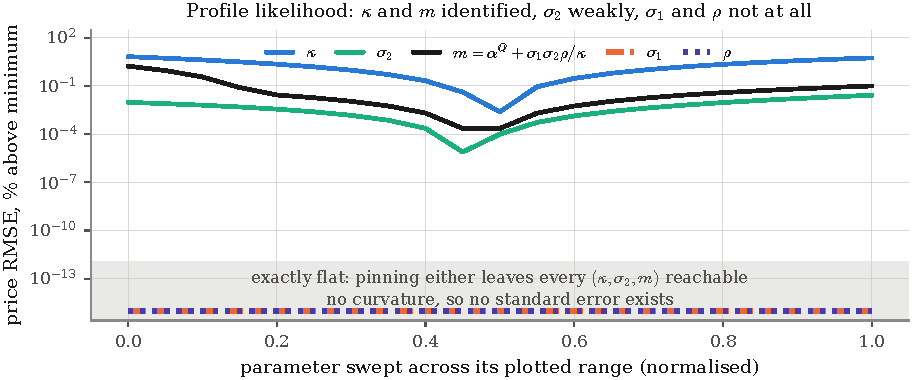
\includegraphics[width=0.94\linewidth]{figures/results/ident1_profile_likelihood.pdf}
        \subcaption{Profile likelihood: each parameter swept across its plotted
        range with the remainder re-optimised. Note the logarithmic vertical
        axis. For $\sigma_1$ and $\rho$ the inner optimisation is solved
        analytically rather than numerically, since pinning either leaves every
        $(\kappa, \sigma_2, m)$ reachable and the objective is indifferent by
        construction; they are drawn at the plotting floor because a
        logarithmic axis cannot represent zero.}
        \label{fig:ident_profile}
    \end{subfigure}

    \vspace{0.35cm}

    \begin{subfigure}[t]{0.62\textwidth}
        \centering
        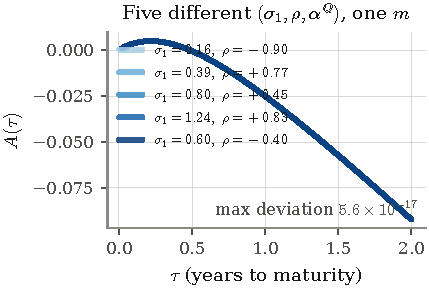
\includegraphics[width=\linewidth]{figures/results/ident2_invariance.pdf}
        \subcaption{The same claim in price space: $A(\tau)$ drawn for five
        $(\sigma_1, \rho, \longrun^{\mathbb{Q}})$ triples sharing one value of
        $m$. Every curve lies on every other.}
        \label{fig:ident_invariance}
    \end{subfigure}
    \caption{Two views of the same structural fact. In (a) the identified
    coordinates $\kappa$ and $m$ show clear curvature and $\sigma_2$ two to
    three orders of magnitude less, while $\sigma_1$ and $\rho$ are exactly
    flat --- there is no curvature from which a standard error could be
    computed. In (b) the consequence is shown directly on the pricing function:
    parameter vectors differing wildly in $\sigma_1$, $\rho$ and
    $\longrun^{\mathbb{Q}}$ produce numerically indistinguishable term
    structures provided $m$ is held fixed.}
    \label{fig:identifiability}
\end{figure}

This bounds the two estimators compared in this thesis differently, and the
distinction is architectural rather than a matter of tuning. The Kalman
filter's measurement equation (Section~\ref{sec:kalman}) inherits exactly the
same rank-three limitation, because it is the same pricing relation. Its
\emph{transition} equation, however, carries information the cross-section does
not: $\sigma_1$ enters the conditional variance of $\Delta x_t$, where
$x_t = \ln S_t$, and $\rho$ the
cross-covariance of the two state innovations, so its likelihood can separate
both. AP-PEN, by contrast, routes all learning of its structural parameters
through the pricing channel -- the $\mathbb{Q}$-group is trained on the
data-misfit loss alone (Section~\ref{sec:alternating}), a purely
cross-sectional objective -- and so structurally cannot identify $\sigma_1$ or
$\rho$ however long it trains. The practical consequence is that the recovered
parameters must be read along the identified coordinates
$(\meanrev, \sigma_2, m)$ rather than one by one; doing otherwise mistakes a
property of the observation equation for an estimation failure
(Section~\ref{sec:synthetic}).

\subsection{Physics-Enforced Inversion}
\label{sec:pinn_inversion}
This paper proposes the Affine-Partitioned, Physics-Enforced Network (AP-PEN), which resolves the inverse tautology problem identified in Section~\ref{sec:gs_model} by splitting the closed-form solution (Equation~\ref{eq:gs_futures}) into an analytically imposed component and a learned component. The name reflects both halves of that split. \emph{Affine-partitioned}: the deterministic affine term-structure map, $A(\tau)$ and $B(\tau)$, is separated from the latent convenience-yield path and imposed exactly, leaving only the path itself to be learned. \emph{Physics-enforced} rather than physics-informed: no differential-equation residual appears anywhere in the loss (Section~\ref{sec:multi_obj}), because the pricing PDE (Eq.~\ref{eq:gs_pde_tau}) is satisfied by construction through that exact imposition, not penalised toward satisfaction as in the Raissi-style residual~\cite{Raissi2019Physics-informedEquations} formulation reviewed in Section~\ref{sec:lit_pinns}. Figure~\ref{fig:appinn} shows the model architecture.

The architecture contains a single network, the path network
$\hat{\delta}_\phi: t \mapsto \hat{\delta}_\phi(t)$, which addresses the inverse
problem at the centre of this thesis: it maps calendar time to an estimated
latent convenience yield. Critically, $\hat{\delta}_\phi$ does not take the
observed futures term structure as an input; the inversion is achieved through
training, not through the network's forward signature. This section details the
architecture; the composite loss function that solves the inverse problem and
optimises pricing accuracy is developed in Section~\ref{sec:multi_obj}.

The model consumes two kinds of numerical input, plus one set of shared
parameters that are not inputs in the conventional sense but enter every
evaluation. The first is the observed data: a panel of daily records
$(S_i, t_i, \{F^{\text{obs}}_{i,k}\}_{k=1}^{N_\tau})$ for $i = 1, \dots, n$,
drawn from the WTI term structures across the sample (the synthetic and real
data formulation is discussed in Section~\ref{sec:experimental_design}). The
second is the maturity grid $\{\tau_k\}_{k=1}^{N_\tau}$, a single vector of
time-to-maturity values, one per contract slot $k$, shared across every
observation date $i$ rather than varying per record.

The shared parameters $\psi = \{\kappa,\ \sigma_1,\ \sigma_2,\ \rho,\ \alpha^{\mathbb{P}}\}$ are learned alongside $\phi$, while the interest rate $r$ and risk premium $\lambda_2$ are held fixed. The full five-parameter set is retained rather than the reduced $(\kappa,\sigma_2,m)$ of Section~\ref{sec:identifiability}: $\alpha^{\mathbb{P}}$ is required by the $\mathbb{P}$-measure transition loss of Section~\ref{sec:multi_obj}, and keeping $\psi$ intact lets the predicted degeneracy in $\sigma_1$, $\rho$ and $\alpha^{\mathbb{Q}}$ be verified empirically rather than assumed. Crucially, the risk-neutral long-run level $\alpha^{\mathbb{Q}}$ is not learned independently. Because $\lambda_2$ and $\alpha^{\mathbb{P}}$ only interact through the measure-change relation $\alpha^{\mathbb{Q}} = \alpha^{\mathbb{P}} - \sigma_2\lambda_2/\kappa$ (Appendix~\ref{app:gs_derivation}), fitting $\alpha^{\mathbb{Q}}$ directly would create an underdetermined system where infinite $(\alpha^{\mathbb{P}}, \lambda_2)$ pairs yield identical losses. Fixing $\lambda_2$ exogenously resolves this, allowing $\alpha^{\mathbb{Q}}$ to be derived at every step directly from the network's fitted $\alpha^{\mathbb{P}}$.

Two qualifications are needed here, since both bear on how the recovered $\psi$ should be read. First, fixing $\lambda_2$ removes only the $(\alpha^{\mathbb{P}}, \lambda_2)$ redundancy just described; it does nothing about the deeper non-identifiability of Section~\ref{sec:identifiability}, which is a property of the closed form itself and survives any reparameterisation of $\psi$. Second, the substitution introduces a pathology of its own in the form of a $1/\kappa$ pole: as $\kappa \to 0$ the term $\sigma_2\lambda_2/\kappa$ diverges, so an arbitrarily small $\kappa$ buys unbounded leverage over $\alpha^{\mathbb{Q}}$ at negligible cost to the pricing fit. The degeneracy compounds, because once $\kappa \approx 0$ the $\mathbb{P}$ transition mean $\alpha^{\mathbb{P}} + (\delta_i - \alpha^{\mathbb{P}})e^{-\kappa\Delta t}$ collapses to $\delta_i$ and $\alpha^{\mathbb{P}}$ drops out of the transition likelihood too, leaving both long-run levels free to drift together in opposite directions.

The learned entries of $\psi$ are accordingly reparameterised so the optimiser itself remains unconstrained: $\sigma_1$ and $\sigma_2$ through a softplus, $\rho$ through a $\tanh$, $\alpha^{\mathbb{P}}$ through the identity, and $\kappa$ through a \emph{floored} softplus, $\kappa = \kappa_{\min} + \mathrm{softplus}(\cdot)$ with $\kappa_{\min} = 0.1$, rather than the plain softplus the other positive parameters use. The floor is not an arbitrary numerical safeguard. Below $\kappa = 0.1$ the mean-reversion half-life $\ln 2/\kappa = 6.9$ years exceeds the longest maturity observed in the WTI panel ($1.88$ years, Table~\ref{tab:data_stats}) by a factor of roughly $3.7$, so $B(\tau) \approx -\tau$ across the entire observable range and the second factor becomes indistinguishable from deterministic cost-of-carry. The floor therefore excludes only a region in which the two-factor structure is already unidentified from this maturity range, rather than constraining an economically meaningful value away from its optimum.

To test whether $\delta$-recovery degrades gracefully under incorrect assumptions about this unobservable risk premium, our synthetic experiments generate data with a true $\lambda_2 = 0.10$ but train with a deliberately misspecified $\lambda_2^{\text{fixed}} = 0.13$ (+30\%). On the real WTI panel, we instead use the Kalman filter's MLE estimate for $\lambda_2$, keeping both methods' assumptions aligned for a fair comparison.

\definecolor{datafill}{RGB}{232,240,250}
\definecolor{datastroke}{RGB}{70,110,160}
\definecolor{netfill}{RGB}{255,255,255}
\definecolor{netstroke}{RGB}{90,90,90}
\definecolor{lossfill}{RGB}{245,238,230}
\definecolor{lossstroke}{RGB}{150,110,70}
\definecolor{sumfill}{RGB}{238,238,238}
\definecolor{anafill}{RGB}{238,234,244}
\definecolor{anastroke}{RGB}{118,98,148}
\definecolor{bpstroke}{RGB}{150,60,55}

\begin{figure*}[!t]
\centering
\resizebox{\textwidth}{!}{%
\begin{tikzpicture}[
    >={Stealth[length=2.2mm]},
    font=\footnotesize,
    flow/.style    ={line width=0.7pt, rounded corners=2.5pt},
    slim/.style    ={line width=0.55pt,rounded corners=2.5pt},
    par/.style     ={line width=0.6pt, draw=anastroke, densely dashed, rounded corners=2.5pt},
    sg/.style      ={line width=0.6pt, draw=netstroke, dash pattern=on 2.4pt off 1.6pt, rounded corners=2.5pt},
    arb/.style     ={line width=0.55pt,draw=lossstroke,densely dashed, rounded corners=2.5pt},
    bp/.style      ={line width=0.75pt,draw=bpstroke,  dashed,          rounded corners=3pt},
    tag/.style     ={font=\scriptsize, inner sep=1.5pt},
    jn/.style      ={circle, fill=black, inner sep=0pt, minimum size=2.4pt},
    dbox/.style    ={draw=datastroke, fill=datafill, rounded corners=2.5pt, line width=0.6pt, align=center, inner sep=3pt},
    abox/.style    ={draw=anastroke,  fill=anafill,  rounded corners=2.5pt, line width=0.6pt, align=center, inner sep=3pt},
    lbox/.style    ={draw=lossstroke, fill=lossfill, rounded corners=2pt,   line width=0.6pt, align=center, inner sep=3pt, text width=36mm},
    cbox/.style    ={lbox, densely dashed},
    sumnode/.style ={draw, fill=sumfill, circle, inner sep=0pt, minimum size=8mm, line width=0.7pt},
]

% ===============================================================
%  LAYOUT CONSTANTS
%  columns: cIn -> cNet -> cTr -> cLoss -> cSum
%  routing channels: xPsi (left), xDel / xFhat (centre), xBP (right)
% ===============================================================
\def\cIn{-0.6}   \def\cNet{3.9}   \def\cTr{7.6}
\def\cLoss{12.4} \def\cSum{15.6}
\def\xPsi{-3.5}  \def\xDel{9.5}   \def\xFhat{9.7}  \def\xBP{17.2}
\def\yBP{7.6}    \def\yTop{6.0}   \def\yNet{3.2}   \def\yMid{1.0}
\def\yAna{-2.0}  \def\yCac{-1.3}  \def\yRcac{-3.2} \def\yPsiBot{-4.5}

% ===============================================================
%  NODES
% ===============================================================
\node[abox,minimum width=36mm,minimum height=20mm] (glob) at (\cIn,\yTop)
     {\textbf{Shared parameters}\\[1pt]
      $\psi=\{\kappa,\sigma_1,\sigma_2,\rho,\alpha^{\mathbb{P}}\}$ \emph{learned}\\[1pt]
      {\scriptsize $\alpha^{\mathbb{Q}}=\alpha^{\mathbb{P}}-\sigma_2\lambda_2/\kappa$ \emph{derived}}\\[-1pt]
      {\scriptsize ($\lambda_2$ fixed)}};

\node[dbox,minimum width=32mm,minimum height=13mm] (data) at (\cIn,\yNet)
     {\textbf{Observed panel}\\[1pt]$(S_i,\,t_i,\,r_i,\,F^{\mathrm{obs}}_{i,k})$};

\node[dbox,minimum width=32mm,minimum height=12mm] (mats) at (\cIn,\yAna)
     {\textbf{Maturity grid}\\[1pt]$\{\tau_k\}_{k=1}^{N_\tau}$};

% --- path network -------------------------------------------------
\node[draw=netstroke,fill=netfill,rounded corners=3pt,line width=0.8pt,
      minimum width=28mm,minimum height=15mm,inner sep=0pt] (pathnet) at (\cNet,\yNet) {};
\begin{scope}[shift={(\cNet,\yNet)}]
  \tikzset{syn/.style={draw=netstroke!50,line width=0.2pt},
           nrn/.style={circle,draw=netstroke,fill=white,minimum size=2.4mm,
                       inner sep=0pt,line width=0.35pt}}
  \coordinate (nin) at (-0.95,0);  \coordinate (nout) at (0.95,0);
  \foreach \k/\yy in {m/-0.34, z/0, p/0.34}{
      \coordinate (a\k) at (-0.32,\yy);  \coordinate (b\k) at (0.32,\yy);}
  \foreach \k in {m,z,p}{\draw[syn] (nin) -- (a\k); \draw[syn] (b\k) -- (nout);}
  \foreach \i in {m,z,p}\foreach \j in {m,z,p}{\draw[syn] (a\i) -- (b\j);}
  \node[nrn] at (nin) {};  \node[nrn] at (nout) {};
  \foreach \k in {m,z,p}{\node[nrn] at (a\k) {}; \node[nrn] at (b\k) {};}
\end{scope}
\node[below=1.2mm of pathnet,align=center] (pathlab)
     {\textbf{Path network} $\hat{\delta}_\phi:\ t\mapsto\hat{\delta}$\\[-2pt]
      {\scriptsize the only trainable network}};

\node[abox,minimum width=34mm,minimum height=15mm] (ABblk) at (\cNet,\yAna)
     {\textbf{Analytic} $A(\tau),\,B(\tau)$\\[1pt]
      {\scriptsize $B(\tau)=-(1-e^{-\kappa\tau})/\kappa$}\\[-1pt]
      {\scriptsize $A(\tau)$: closed form, Eq.~\ref{eq:app_A}}};

\node[abox,minimum width=32mm,minimum height=14mm] (trans) at (\cTr,\yMid)
     {\textbf{Pricing transform}\\[2pt]
      $\hat{F}=S\,e^{\,B(\tau)\hat{\delta}+A(\tau)}$};

% --- loss channels ------------------------------------------------
\node[lbox,minimum height=16mm] (lsde) at (\cLoss,\yTop)
     {$\hat{\mathcal{L}}_{\mathrm{SDE}}$: transition NLL ($\mathbb{P}$, OU)\\[1pt]
      {\scriptsize $-\log p(\hat{\delta}_{i+1}\mid\hat{\delta}_i;\psi)$}\\[-1pt]
      {\scriptsize updates $\alpha^{\mathbb{P}}$ only (Step 2b)}};

\node[cbox,minimum height=14mm] (ldelta) at (\cLoss,\yNet)
     {$\hat{\mathcal{L}}_{h,\delta}$: convenience-yield floor\\[1pt]
      {\scriptsize on $\hat{\delta}_\phi(t_i)$ directly}};

\node[lbox,minimum height=14mm] (ldata) at (\cLoss,\yMid)
     {$\hat{\mathcal{L}}_{\mathrm{data}}$: data misfit\\[1pt]
      {\scriptsize $\|\ln\hat{F}_{i,k}-\ln F^{\mathrm{obs}}_{i,k}\|^2$}};

\node[cbox,minimum height=13mm] (lcac) at (\cLoss,\yCac)
     {$\hat{\mathcal{L}}_{h,\mathrm{cac}}$: cash-and-carry hinge\\[1pt]
      {\scriptsize $\hat{F}_{i,k}$ vs.\ $S_ie^{(r_i+u)\tau_k}$}};

\node[cbox,minimum height=13mm] (lrcac) at (\cLoss,\yRcac)
     {$\hat{\mathcal{L}}_{h,\mathrm{rcac}}$: reverse cash-and-carry hinge\\[1pt]
      {\scriptsize $\hat{F}_{i,k}$ vs.\ $S_ie^{(r_i-\delta_{\max})\tau_k}$}};

\node[sumnode] (sum) at (\cSum,\yMid) {$\Sigma$};

\node[abox,minimum width=28mm,minimum height=16mm] (wamol) at (\cSum,-5.3)
     {\textbf{WamOL}\\[1pt]{\scriptsize channel-level}\\[-1pt]
      {\scriptsize loss balancing}\\[-1pt]
      {\scriptsize (Step 1, every 100 epochs)}\\[-1pt]
      {\scriptsize \emph{inert unless ARB active}}};

% ===============================================================
%  FORWARD EDGES
% ===============================================================
% inputs
\draw[->,flow] (data.east) -- node[tag,above]{$t_i$} (pathnet.west);
\draw[->,flow] (data.south) |- node[tag,above,pos=0.78]{$S_i,\,r_i$} (trans.west);
\draw[->,slim] (mats.east) -- node[tag,above,pos=0.4]{$\tau_k$} (ABblk.west);

% psi bus: glob -> SDE loss, with a hop over the backprop drop.
% The second tag matters: e_SDE READS kappa and sigma_2 but cannot WRITE them
% (both stop-gradiented inside the channel), so only alpha^P is trained here.
\draw[->,par,sharp corners]
      (glob.east) -- node[tag,above,pos=0.08]{$\psi$} (4.42,\yTop)
      arc (180:0:0.18)
      -- node[tag,above,pos=0.62]{\scriptsize $\kappa,\sigma_2$ stop-grad} (lsde.west);
% psi -> analytic block, down the left-hand channel
\draw[->,par] (glob.west) -- (\xPsi,\yTop) -- node[tag,right,pos=0.38]{$\psi$}
      (\xPsi,\yPsiBot) -- (\cNet,\yPsiBot) -- (ABblk.south);

% delta-hat bus
\draw[flow] (pathnet.east) -- node[tag,above,pos=0.10]{$\hat{\delta}$} (\xDel,\yNet);
\node[jn] at (\cTr,\yNet) {};  \node[jn] at (\xDel,\yNet) {};
\draw[->,flow] (\cTr,\yNet) -- (trans.north);
\draw[->,arb]  (\xDel,\yNet) -- (ldelta.west);
\draw[->,sg]   (\xDel,\yNet) -- (\xDel,4.4)
               -- node[tag,above]{$\hat{\delta}$ (stop-grad)} (\cLoss,4.4) -- (lsde.south);

% analytic -> pricing transform
\draw[->,flow] (ABblk.east) -| node[tag,above,pos=0.28]{$A,B$} (trans.south);

% F-hat bus
\draw[->,flow] (trans.east) -- node[tag,above]{$\hat{F}_{i,k}$} (ldata.west);
\node[jn] at (\xFhat,\yMid) {};  \node[jn] at (\xFhat,\yCac) {};
\draw[arb]     (\xFhat,\yMid) -- (\xFhat,\yRcac);
\draw[->,arb]  (\xFhat,\yCac)  -- (lcac.west);
\draw[->,arb]  (\xFhat,\yRcac) -- (lrcac.west);

% ===============================================================
%  LOSS AGGREGATION
% ===============================================================
\draw[->,slim] (lsde.east)   -| node[tag,above,pos=0.20]{$\lambda_{\mathrm{SDE}}$}  (sum.75);
\draw[->,arb]  (ldelta.east) -| (sum.135);
\draw[->,slim] (ldata.east)  -- node[tag,above]{$\lambda_{\mathrm{data}}$} (sum.west);
\draw[->,arb]  (lcac.east)   -| (sum.225);
\draw[->,arb]  (lrcac.east)  -| (sum.265);
\draw[->,par]  ([xshift=10mm]wamol.north) |- node[tag,right,pos=0.18]{$\lambda_\beta$} (sum.320);
\draw[->,flow] (sum.east) -- node[tag,above]{$\hat{\mathcal{L}}$} (\xBP,\yMid);
\node[jn] at (\xBP,\yMid) {};

% ===============================================================
%  BACKPROPAGATION PATH
% ===============================================================
\draw[->,bp] (\xBP,\yMid) -- (\xBP,\yBP)
     -- node[above,font=\scriptsize,text=bpstroke,pos=0.62]
        {backprop:\ $\phi$ (Step 1)\ $\mid$\ $\{\kappa,\sigma_1,\sigma_2,\rho\}$ (Step 2a)\ $\mid$\ $\alpha^{\mathbb{P}}$ (Step 2b)}
     (\cIn,\yBP) -- (glob.north);
\draw[->,bp] (4.6,\yBP) -- (4.6,3.95);

% ===============================================================
%  LEGEND
% ===============================================================
\begin{scope}[shift={(\xPsi,-5.3)},font=\scriptsize,
              key/.style={rounded corners=1.5pt,line width=0.7pt,
                          minimum width=5mm,minimum height=3mm,inner sep=0pt}]
  \node[key,draw=netstroke,  fill=netfill]  (k1) at (0,0)   {};
  \node[anchor=west,inner sep=1.5pt] at (k1.east) {learned network};
  
  \node[key,draw=anastroke,  fill=anafill]  (k2) at (3.0,0) {}; 
  \node[anchor=west,inner sep=1.5pt] at (k2.east) {imposed structure / parameters};
  
  \node[key,draw=datastroke, fill=datafill] (k3) at (7.8,0) {}; 
  \node[anchor=west,inner sep=1.5pt] at (k3.east) {input data};
  
  \node[key,draw=lossstroke, fill=lossfill] (k4) at (10.0,0) {}; 
  \node[anchor=west,inner sep=1.5pt] at (k4.east) {loss channel};
  
  \node[key,draw=lossstroke, fill=lossfill,densely dashed] (k5) at (12.5,0) {}; 
  \node[anchor=west,inner sep=1.5pt] at (k5.east) {AP-PEN (ARB) only};
\end{scope}

\end{tikzpicture}%
}
\caption{The AP-PEN architecture. The observed panel $(S_i, t_i, r_i, F^{\mathrm{obs}}_{i,k})$
and the fixed maturity grid $\{\tau_k\}_{k=1}^{N_\tau}$ feed the path network
$\hat{\delta}_\phi$ and the analytic block respectively, while the shared
parameters $\psi = \{\kappa, \sigma_1, \sigma_2, \rho, \alpha^{\mathbb{P}}\}$
(with $\alpha^{\mathbb{Q}}$ derived) are broadcast to both. $\hat{\delta}_\phi$
is the only learned network in the architecture: it maps calendar time to the
estimated convenience yield $\hat{\delta}$, which combines with the
analytically imposed $A(\tau)$ and $B(\tau)$ in the pricing transform to give
the model futures price $\hat{F}_{i,k}$. Five loss channels follow: the
data-misfit and SDE transition-NLL channels (solid boxes, active in every
variant) and three hinge losses (dashed boxes, active only in
AP-PEN (ARB)) covering cash-and-carry arbitrage, reverse cash-and-carry
arbitrage, and a convenience-yield floor acting directly on $\hat{\delta}_\phi$
rather than on $\hat{F}_{i,k}$. Active channels are summed into
$\hat{\mathcal{L}}$ and balanced by the WamOL gradient-norm scheme
(Section~\ref{sec:multi_obj}); note that for the unconstrained variants the
balancer is inert by construction, since
$\hat{\mathcal{L}}_{\mathrm{SDE}}$'s gradient into $\phi$ is severed and only
one channel remains live in Step 1. Backpropagation then updates disjoint
parameter groups across three alternating steps: $\phi$ against the full
weighted loss, $\{\kappa, \sigma_1, \sigma_2, \rho\}$ against the data-misfit
channel alone, and $\alpha^{\mathbb{P}}$ against the transition-NLL channel
alone (Section~\ref{sec:alternating}). Solid arrows carry tensors, dashed
purple arrows carry shared parameters, and the dashed red path traces the
gradient route together with the parameter group updated at each step.}
\label{fig:appinn}
\end{figure*}

No-arbitrage and economic bounds are introduced as additional loss terms in Section~\ref{sec:constraints}, separate from the base composite objective and as a direct extension of the derivative-constrained loss terms developed in~\cite{Hoshisashi2024Physics-InformedPDEs}.

The path network's output is combined with the analytic $A(\tau)$ and
$B(\tau)$ through a pricing transform that is fixed, not learned:
\begin{equation}
    \label{eq:pricing_transform}
    \hat{F}(S, \hat{\delta}, \tau) = S \exp\!\big(B(\tau)\,\hat{\delta} +
    A(\tau)\big), \qquad
    B(\tau) = -\frac{1-e^{-\kappa\tau}}{\kappa}.
\end{equation}

For every observed maturity $\tau$, fixing the shared parameter set $\psi$ pins down
both $A(\tau)$ and $B(\tau)$ as functions of $\tau$ alone: each simultaneously
solves an initial value problem in the single variable $\tau$
(Equations~\ref{eq:gs_ode_B} and~\ref{eq:gs_ode_A}), with a unique solution
existing for every $\tau \geq 0$. The latent state $\delta_t$, by contrast, is
not the solution of an initial value problem; it is the realised path of a
stochastic process (Equation~\ref{eq:gs_cy}) and is not analytically computable
from $\psi$ and $t$ alone, since fixing $\psi$ pins down $\delta_t$ only given
an entire, unobserved realisation of the driving Brownian motion
$W_2^{\mathbb{P}}$.

The log-futures relation is linear in $\delta$,
$\ln\hat{F} - \ln S - A(\tau) = B(\tau)\,\delta$ (Equation~\ref{eq:gs_futures}),
and is therefore directly invertible via least squares at each observation
date. This per-date approach, however, treats every date as an independent
inverse problem and uses no information from neighbouring dates, discarding by
construction the continuous, mean-reverting structure that $\delta$ is known to
obey (Equation~\ref{sde2}); it also cannot produce a value between observation
dates. A network trained on $t \mapsto \hat\delta_\phi(t)$ across the full
sample is, by contrast, structurally capable of pooling information across
dates through its own inductive bias, and can additionally absorb the DC-PINN
hinge losses (Section~\ref{sec:constraints}) directly on the recovered path,
which the Kalman filter's linear-Gaussian formulation (Section~\ref{sec:kalman})
cannot accommodate without losing tractability. Whether this pooling capacity
yields a materially better estimate of $\delta_t$ than the per-date baseline
(formalised as an evaluated benchmark in Section~\ref{sec:ls_baseline})
is an empirical question addressed in Section~\ref{sec:synthetic}.

The departure from the Raissi-style PINN~\cite{Raissi2019Physics-informedEquations} follows from the tautology argument
discussed in Section~\ref{sec:gs_model}. In the classical PINN formulation,
the network solves an inverse problem by encoding the model's physics into
the loss via a PDE residual. Such an approach would be vacuous here: the PDE
residual is a statement about $\hat{F}$ over the whole $(S, \delta, \tau)$
domain, and is satisfied by the true pricing function regardless of the
market's realised $\delta$ path, so it carries no information about the
latent state. The architecture instead partitions the closed-form solution:
both $B(\tau)$, the channel through which $\delta$ enters pricing, and
$A(\tau)$ are fixed analytically, leaving only the latent path
$\hat\delta_\phi$ to be learned.

\subsection{Composite Objective and Loss Balancing}
\label{sec:multi_obj}

The composite loss function $\hat{\mathcal{L}}$ combines two loss channels
adapted to the single-network Gibson--Schwartz architecture described above: a
data-fit loss and a path transition negative-log-likelihood (NLL) loss. Unlike
the four-term structure of the DC-PINN framework
(data, boundary/IC, PDE residual, no-arbitrage)~\cite{Hoshisashi2024Physics-InformedPDEs},
the boundary condition here is enforced as a hard architectural constraint
rather than a trained loss term, no differential-equation residual remains in
the loss at all (Section~\ref{sec:pinn_inversion}), and no-arbitrage and
storage-cost penalties are introduced separately in Section~\ref{sec:constraints}
rather than in the base composite below. $\hat{\mathcal{L}}_{\text{data}}$ retains the
mean-squared-error form of Hoshisashi et al.~\cite{Hoshisashi2024Physics-InformedPDEs}
but is evaluated against the predicted prices $\hat{F}_{i,k}$ and the observed futures
prices $F^{\text{obs}}_{i,k}$.

\begin{equation}
\hat{\mathcal{L}} :=
\underbrace{\lambda_{\text{data}} \hat{\mathcal{L}}_{\text{data}}}_{\text{Data misfit}}
+ \underbrace{\lambda_{\text{SDE}} \hat{\mathcal{L}}_{\text{SDE}}}_{\text{Path transition negative log-likelihood}}.
\label{eq:composite}
\end{equation}

The non-negative weights $\lambda_{\text{data}}$ and $\lambda_{\text{SDE}}$ control the relative importance of each loss channel. Because fixed weights often allow one loss term to dominate during training (Section~\ref{sec:lit_wamol}), we dynamically adjust them \cite{Hoshisashi2024Physics-InformedPDEs}. Rather than using the original DC-PINN's complex per-point scheme, we apply a channel-level gradient-norm balancing rule: weights are periodically recomputed and smoothed via momentum to ensure both channels produce gradient updates of comparable magnitude.

Furthermore, the two channels route gradients to disjoint subsets of the physical parameters $\psi = \{\kappa, \sigma_1, \sigma_2, \rho, \alpha^{\mathbb{P}}\}$ (where $\alpha^{\mathbb{Q}}$ is derived, Section~\ref{sec:pinn_inversion}). By using separate optimiser states, the data-misfit channel exclusively updates $\{\kappa, \sigma_1, \sigma_2, \rho\}$, while the SDE channel exclusively updates $\alpha^{\mathbb{P}}$.

The data-fit loss $\hat{\mathcal{L}}_{\text{data}}$ is evaluated at each of
the $N_t$ observation dates $i$ and each of the $N_\tau$ observed maturities
$k$, where the model price is computed from the spot $S_i$, the estimated
convenience yield $\hat{\delta}_\phi(t_i)$, and the time-to-maturity
$\tau_k$, via the fixed pricing transform:

\begin{equation}
    \hat{F}_{i,k} := \hat{F}\big( S_i,\ \hat{\delta}_\phi(t_i),\ \tau_k \big)
    = S_i \exp\!\big( B(\tau_k)\,\hat{\delta}_\phi(t_i) + A(\tau_k) \big).
    \label{eq:fik-def}
\end{equation}

Because $A(\tau)$ is imposed as the exact closed form
(Equation~\ref{eq:app_A}) rather than left as a free network output,
every entry of $\psi$ enters the data-misfit channel, not just $\kappa$:
$\kappa$ appears in $B(\tau)$ and in every term of $A(\tau)$; $\sigma_1$
and $\rho$ enter only through the $\sigma_1\sigma_2\rho$ cross-term;
$\sigma_2$ enters both through its own variance terms and through
$\alpha^{\mathbb{Q}}$; and $\alpha^{\mathbb{P}}$ enters only indirectly,
substituted through
$\alpha^{\mathbb{Q}} = \alpha^{\mathbb{P}} - \sigma_2\lambda_2/\kappa$
(Section~\ref{sec:pinn_inversion}). This design choice does not resolve
$\alpha^{\mathbb{P}}$ against $\lambda_2$: because $\alpha^{\mathbb{P}}$
appears only bundled inside $\alpha^{\mathbb{Q}}$, the data loss alone
cannot separate the two, so $\lambda_2$ is held fixed rather than learned.

To ensure the model output enters the pricing transform linearly, we take
the futures prices in log form: $\ln\hat{F}$ is an affine function of
$\hat{\delta}$ via $B(\tau)$, rather than the multiplicative, non-linear
relationship that Eq.~\ref{eq:fik-def} would otherwise
impose on the raw price. The data-misfit loss is then the mean squared error
of this log-price residual, which is quadratic in $\hat{\delta}$ rather than linear.

\begin{equation}
\hat{\mathcal{L}}_{\text{data}} = \frac{1}{N_t N_\tau} \sum_{i=1}^{N_t} \sum_{k=1}^{N_\tau}
\left\lVert \ln \hat{F}_{i,k} - \ln F^{\text{obs}}_{i,k} \right\rVert^2.
\label{eq:data-loss}
\end{equation}

As identified in Section~\ref{sec:pinn_inversion}, the PDE
residual $\hat{\mathcal{L}}_f$ in
DC-PINN/WamOL~\cite{Hoshisashi2024Whack-a-moleSurface,
Hoshisashi2024Physics-InformedPDEs} has no analogue in AP-PEN and is
omitted. Beyond the identifiability argument made there, a stronger
structural reason applies: $A(\tau)$ and $B(\tau)$ are the closed-form
solutions of Equations~\ref{eq:gs_ode_B}--\ref{eq:gs_ode_A} for arbitrary
$\psi$ (Appendix~\ref{app:gs_pde}), so the pricing PDE
(Eq.~\ref{eq:gs_pde_tau}) is satisfied identically under this
parameterisation, independent of $\psi$, by construction rather than by
penalty. The same closed form gives $A(0) = B(0) = 0$, so the initial
condition $\hat{F}(S,\delta,0) = S$ likewise holds identically, which is
why Equation~\ref{eq:composite} carries no boundary-condition term
$\hat{\mathcal{L}}_b$ either.

The SDE channel uses the Ornstein-Uhlenbeck (OU) process (Eq.~\ref{sde2}) to constrain the estimated path $\delta_t$ to its mean-reverting dynamics under $\mathbb{P}$. Unlike the data loss, this channel updates only $\alpha^{\mathbb{P}}$, using the path network's output without altering its weights. Because Eq.~\ref{sde2} is linear, it admits a closed-form transition density over each time step $\Delta t$ between consecutive observation dates:

\begin{equation}
\begin{gathered}
  \delta_{t+\Delta t} \mid \delta_t \sim \mathcal{N}\!\big(m(\delta_t, \Delta t),\, v(\Delta t)\big), \\
  m(\delta_t, \Delta t) = \alpha^{\mathbb{P}} + \big(\delta_t - \alpha^{\mathbb{P}}\big)\,e^{-\kappa \Delta t}, \qquad
  v(\Delta t) = \frac{\sigma_2^2}{2\kappa} \Big(1 - e^{-2\kappa \Delta t}\Big).
\end{gathered}
\end{equation}

Here, $\mathcal{N}(m, v)$ denotes the normal distribution of the OU transition law~\cite{uhlenbeck1930theory} with mean $m$ and variance $v$. 

Writing $m_i \coloneqq m(\hat{\delta}_i, \Delta t_i)$ and $v_i \coloneqq v(\Delta t_i)$, the per-step negative log-likelihood is directly derived from the Gaussian density:

\begin{equation}
    \ell_{\text{SDE}}[\hat{\delta}_\phi, \psi]\big( t_i, t_{i+1} \big)
    = \frac{1}{2}\log\!\big(2\pi\, v_i\big)
      + \frac{\big(\hat{\delta}_{i+1} - m_i\big)^2}{2\,v_i}.
\end{equation}

Averaging this across all $N_p$ steps yields the total SDE loss:

\begin{equation}
    \hat{\mathcal{L}}_{\text{SDE}} = \frac{1}{N_p}
  \sum_{i=1}^{N_p}
    \ell_{\text{SDE}}[\hat{\delta}_\phi, \psi]\big( t_i, t_{i+1} \big).
\end{equation}

Although $\hat{\mathcal{L}}_{\text{SDE}}$ depends on multiple variables, it exclusively trains $\alpha^{\mathbb{P}}$. We apply stop-gradients to $\kappa$, $\sigma_2$, and the network-smoothed path $\hat\delta_\phi$ for two reasons: first, $\kappa$ and $\sigma_2$ are already identified by the data-fit channel, and updating them here would cause a degenerate fit ($\kappa \to 0$); second, this SDE channel is not meant to train the network weights $\phi$. 

Consequently, $\alpha^{\mathbb{P}}$ is the sole parameter updated here, and it only influences the data-fit channel indirectly via the derived $\alpha^{\mathbb{Q}}$ (Section~\ref{sec:pinn_inversion}). Finally, because each loss term pairs consecutive observation dates ($N_t$), there are $N_p = N_t - 1$ terms in total. The underlying Ornstein--Uhlenbeck transition density, from which this negative log-likelihood is read off directly, is derived in Appendix~\ref{app:gs_derivation}.

\subsubsection{Parameter Segregation}
\label{sec:alternating}

Rather than updating the path network and all five learned physics
parameters at each epoch, training is split into three sequential steps:
\begin{itemize}
    \item \textbf{Step 1:} Freeze $(\kappa, \sigma_1, \sigma_2, \rho,
    \alpha^{\mathbb{P}})$ and update the path network $\hat{\delta}_{\phi}$
    against the full weighted loss.
    \item \textbf{Step 2(a):} Update $(\kappa, \sigma_1, \sigma_2, \rho)$
    using only the pricing loss $\hat{\mathcal{L}}_{\text{data}}$;
    $\hat{\delta}_{\phi}$ is frozen. Although $\kappa$ and $\sigma_2$ also
    enter the $\mathbb{P}$ transition density in Step 2(b), they are
    measure-invariant and receive their only gradient update here, not there.
    \item \textbf{Step 2(b):} Update the sole $\mathbb{P}$-specific parameter
    $\alpha^{\mathbb{P}}$ using only the path loss
    $\hat{\mathcal{L}}_{\text{SDE}}$; everything else, including $\kappa$ and
    $\sigma_2$, is frozen via stop-gradient.
\end{itemize}
This segregation is a measure-discipline device rather than an identification
one: it prevents the real-world ($\mathbb{P}$) and risk-neutral ($\mathbb{Q}$)
parameter groups (identified from different, and at times conflicting,
information) from being pulled in inconsistent directions within a single
update. It should not be read as guaranteeing that each step sees exactly the
information that identifies the parameters it trains. That holds for Step 2(b),
whose sole parameter $\alpha^{\mathbb{P}}$ is identified by the transition
density alone, but only partly for Step 2(a): the data-misfit loss identifies
$\kappa$ and $\sigma_2$ (together with the composite $m$ of
Equation~\ref{eq:identified_composite}), while $\sigma_1$ and $\rho$ are
updated in that step despite being structurally unidentified from any purely
cross-sectional objective (Section~\ref{sec:identifiability}).

Each of the three steps is also carried out with its own separate Adam
optimiser state, rather than one shared state in which a frozen group's
gradient is simply masked to zero. Adam smooths every update using a
running average of that parameter's past gradient~\cite{kingma2014adam}; feeding it a zero gradient still updates this average, and so would erode a frozen group's
momentum even though its parameters have not moved. Keeping three fully
separate optimiser states instead means a frozen group is skipped outright
rather than nudged toward zero, so its momentum is preserved exactly until
the step that next trains it.

\subsubsection{Self-Adaptive Loss Balancing}

The balancing of the composite loss $\hat{\mathcal{L}}$ follows the WamOL algorithm~\cite{Hoshisashi2024Whack-a-moleSurface}. This applies only during Step 1 of the alternating optimisation (Section~\ref{sec:alternating}); Steps 2(a) and 2(b) train against single loss channels and require no balancing. Every 100 epochs, we measure the relative strength of each channel $k \in \{\text{data}, \text{SDE}\}$ using its mean absolute gradient with respect to its parameter support $\Theta_k$ (Section~\ref{sec:multi_obj}):

\begin{equation}
g_k(p) := \overline{\big\lvert \nabla_{\Theta_k} \hat{\mathcal{L}}_k(p) \big\rvert}.
\label{eq:gradnorm}
\end{equation}

We use the absolute mean rather than the squared norm of Hoshisashi et al.~\cite{Hoshisashi2024Physics-InformedPDEs} to prevent outlier gradients from dominating during later training stages. The channel weights are then updated via:

\begin{equation}
\lambda_k(p+1) = m_\lambda\,\lambda_k(p) + (1-m_\lambda)\, w_k(p),
\qquad
w_k(p) =
\begin{cases}
1, & \text{if } g_k(p) = 0, \\[4pt]
\dfrac{\sum_{j} g_j(p)}{g_k(p)}, & \text{otherwise},
\end{cases}
\label{eq:lambda-update}
\end{equation}

where $m_\lambda \in [0,1)$ is the momentum ($m_\lambda=0.5$ here; the subscript distinguishes it from the identified composite $m$ of Equation~\ref{eq:identified_composite}), and $j$ indexes all active channels (which expands to $\{\text{data}, \text{SDE}, h\text{-cac}, h\text{-rcac}, h\text{-}\delta\}$ for the AP-PEN (ARB) variant in Section~\ref{sec:constraints}). 

Equation~\ref{eq:lambda-update} generalises the scheme in~\cite{Hoshisashi2024Physics-InformedPDEs} by introducing tunable momentum. This applies an exponential moving average (EMA) to smooth the channel weights, cleanly defining the balance between old and new weights (e.g., $m_\lambda=0.5$ retains 50\% of the previous weight). Additionally, if a gradient momentarily vanishes ($g_k(p)=0$), the momentum smoothly nudges $\lambda_k$ toward 1 rather than hard-resetting it.

Because the stop-gradient severs $\hat{\mathcal{L}}_{\text{SDE}}$'s gradient into $\phi$ (Section~\ref{sec:multi_obj}), this channel contributes nothing to Step 1. During Step 1, $\psi$ is frozen, meaning the target parameter support $\Theta_{\text{SDE}}$ reduces strictly to $\phi$. Consequently, $g_{\text{SDE}}$ is exactly zero and drops out of the balancing weights.

For the standard AP-PEN variant, this leaves $\hat{\mathcal{L}}_{\text{data}}$ as the single active channel in Step 1. The balancer may therefore have no material effect on path recovery, a consequence we test empirically in Section~\ref{sec:synthetic}. However, this limitation vanishes in the AP-PEN (ARB) variant: the no-arbitrage hinge terms ($\hat{\mathcal{L}}_{h,\text{cac}}$, $\hat{\mathcal{L}}_{h,\text{rcac}}$, $\hat{\mathcal{L}}_{h,\delta}$) introduced in Section~\ref{sec:constraints} maintain live gradients into $\phi$, allowing the balancer to actively manage multiple channels.

\subsection{No-Arbitrage and Economic Constraints}
\label{sec:constraints}
While $\hat{\mathcal{L}}_{\text{data}}$ and $\hat{\mathcal{L}}_{\text{SDE}}$ constrain the network to GS dynamics, neither guarantees the inferred convenience yield $\hat{\delta}_{\phi}$ remains economically rational. To prevent paths that fit the pricing dynamics but violate investor constraints, we introduce an additional loss term, $\hat{\mathcal{L}}_{h}$, generalising the derivative constraints of~\cite{Hoshisashi2024Physics-InformedPDEs} into commodity-specific economic and no-arbitrage inequalities.

These model-free inequalities act independently of the GS dynamics. Following~\cite{zhang2025exact}, we enforce them using a one-sided hinge penalty for constraint violations:
\begin{equation}
\hat{\mathcal{L}}_h = \frac{1}{N} \sum_{i=1}^{N}
\big[ \max\!\big(0, -g(x_i)\big) \big]^2.
\label{eq:hinge}
\end{equation}

The cash-and-carry bounds prevent risk-free profits. Cash-and-carry arbitrage occurs when futures are overpriced relative to spot, allowing a trader to borrow at the risk-free rate, buy the physical asset, and short the future. Reverse cash-and-carry exploits the opposite scenario. Both are evaluated on the same $N_t \times N_\tau$ grid as $\hat{\mathcal{L}}_{\text{data}}$, reusing $\hat{F}_{i,k}$ from Equation~\ref{eq:fik-def}.

The interest rate $r$, annualised storage cost $u = 0.30$, and convenience yield ceiling $\delta_{\max} = 0.75$ are fixed constants acting as deliberately loose outer guardrails. $\delta_{\max} = 0.75$ accommodates extreme short-term yields during market turmoil, which Gibson and Schwartz observed approaching $100\%$~\cite{Gibson1990StochasticClaims}. Similarly, $u = 0.30$ safely exceeds baseline storage costs, which average $6$--$9\%$ annualised~\cite{stancu2021dynamics, Fama1987CommodityStorage, byun2017speculation}. It also comfortably exceeds the extreme physical storage spikes seen during the April 2020 oil crash, which reached an implied $13$--$22\%$ annualised.\footnote{During the April 2020 crisis, Cushing physical storage lease rates spiked to roughly \$0.50--\$0.55 per barrel per month \cite{CME2020, Reuters2020}. Annualising this (\$6.00--\$6.60/year) against contemporaneous March/May 2020 spot prices of approximately \$27--\$46/bbl yields an implied storage cost of roughly 13--22\% of spot.}

While both constants are literature-consistent in the sense above, we also
cross-checked the specific values against the violation rates they induce on
the same WTI panel used for evaluation, which is a mild use of information from
the evaluation sample and is acknowledged as such. We initially tested a
regime-switching approach that dynamically widened these bounds during crisis years (2015, 2016, and 2020, where a tighter $u=0.10$ is frequently violated). However, an ablation study showed no measurable difference in path recovery once training fully converged. We therefore adopted the simpler approach of using universally safe, fixed constants.

Because $r$, $u$, and $\delta_{\max}$ are fixed, $\kappa$ is the only learned parameter influencing these terms (via $\hat{F}_{i,k}$). We enforce these arbitrage boundaries through the following two losses:


\begin{equation}
\hat{\mathcal{L}}_{h,\text{cac}} = \frac{1}{N_t N_\tau} \sum_{i=1}^{N_t} \sum_{k=1}^{N_\tau}
\Big[ \max\!\Big( 0,\ \hat{F}_{i,k} - S_i\, e^{(r+u)\tau_k} \Big)
\Big]^2,
\label{eq:cac-loss}
\end{equation}
\begin{equation}
\hat{\mathcal{L}}_{h,\text{rcac}} = \frac{1}{N_t N_\tau} \sum_{i=1}^{N_t} \sum_{k=1}^{N_\tau}
\Big[ \max\!\Big( 0,\ S_i\, e^{(r - \delta_{\max})\tau_k}
- \hat{F}_{i,k} \Big) \Big]^2.
\label{eq:rcac-loss}
\end{equation}

A third hinge acts directly on the latent path to enforce a convenience-yield floor, $\delta_{\min}$. Because the OU process (Equation~\ref{eq:gs_cy}) has unbounded support, neither $\hat{\mathcal{L}}_{\text{data}}$ nor $\hat{\mathcal{L}}_{\text{SDE}}$ prevents $\hat{\delta}_\phi$ from drifting arbitrarily negative.

While idealised models assume a theoretical floor of $\delta \geq 0$~\cite{Liu2009No-ArbitrageStructures}, enforcing this would artificially bias the model during deep-contango regimes (such as the April 2020 storage-exhaustion crisis, which produced sharply negative yields~\cite{Reuters2020, CME2020}). Instead, we set a loose empirical guardrail of $\delta_{\min} = -0.30$, derived from the lower edge of the simulated paths in Section~\ref{sec:experimental_design}.

Like the cash-and-carry bounds, this constraint is enforced via the one-sided squared hinge penalty (Eq.~\ref{eq:hinge}) at every observation date $t_i$. However, it depends solely on the path, without involving spot prices or maturities:
\begin{equation}
\hat{\mathcal{L}}_{h,\delta} = \frac{1}{N_t} \sum_{i=1}^{N_t}
\Big[ \max\!\Big( 0,\ \delta_{\min} - \hat{\delta}_\phi(t_i) \Big) \Big]^2.
\label{eq:delta-floor-loss}
\end{equation}

Hence the full composite loss function for the AP-PEN (ARB) architecture is,

\begin{equation}
\hat{\mathcal{L}} :=
\lambda_{\text{data}} \hat{\mathcal{L}}_{\text{data}}
+ \lambda_{\text{SDE}} \hat{\mathcal{L}}_{\text{SDE}}
+ \lambda_{h,\text{cac}} \hat{\mathcal{L}}_{h,\text{cac}}
+ \lambda_{h,\text{rcac}} \hat{\mathcal{L}}_{h,\text{rcac}}
+ \lambda_{h,\delta} \hat{\mathcal{L}}_{h,\delta}.
\label{eq:composite-full}
\end{equation}

When the no-arbitrage terms are active, $\lambda_{h,\text{cac}}$, $\lambda_{h,\text{rcac}}$ and $\lambda_{h,\delta}$ are balanced by the same gradient-norm mechanism of Equations~\ref{eq:gradnorm}--\ref{eq:lambda-update}, with the channel index $k$ there extended to range over $\{\text{data}, \text{SDE}, h\text{-cac}, h\text{-rcac}, h\text{-}\delta\}$ rather than the two-channel set of Section~\ref{sec:multi_obj}; they are not fixed weights.

\subsection{Closed-Form Least-Squares Baseline}
\label{sec:ls_baseline}

Because $\ln \hat{F}$ is linear in $\delta_t$
(Equation~\ref{eq:pricing_transform}), the inversion admits a closed-form
solution at each date for any fixed $\psi$, with neither a network nor any
gradient training. Minimising the log-price residual of
Equation~\ref{eq:data-loss} over the single scalar $\delta_t$ gives the
per-date ordinary least-squares estimate
\begin{equation}
  \label{eq:ls_delta}
  \hat{\delta}^{\text{LS}}_t
  = \frac{\sum_{k=1}^{N_\tau} B(\tau_k)\big(
      \ln F^{\text{obs}}_{t,k} - \ln S_t - A(\tau_k)\big)}
         {\sum_{k=1}^{N_\tau} B(\tau_k)^2}.
\end{equation}
Profiling $\psi$ out on top of this -- over the identified coordinates
$(\kappa, \sigma_2, m)$ of Section~\ref{sec:identifiability}, the only ones the
cross-section can move -- yields the exact maximum-likelihood estimator of the
whole model under i.i.d.\ Gaussian log-price noise
(Equation~\ref{eq:noise-model}).

This is included as a benchmark because it is the natural control on whether
the neural parameterisation earns its place: it is what AP-PEN reduces to if
the path network contributes nothing beyond a per-date fit. What it gives up is
precisely what Section~\ref{sec:pinn_inversion} argues the network buys --
pooling across neighbouring dates through the network's inductive bias, values
between observation dates, and the hinge penalties of
Section~\ref{sec:constraints} acting directly on the recovered path, none of
which a date-by-date solve can express.

\subsection{Kalman Filter Baseline}
\label{sec:kalman}

Because the path network $\hat{\delta}_\phi$ trains on the full sample, AP-PEN acts as a \textit{smoother} with access to future information. In contrast, the Kalman filter (KF) baseline~\cite{Schwartz1997TheHedging} is causal, using information only up to $t_i$. Any performance gap between the methods stems partly from this asymmetry. A true like-for-like comparison requires the non-causal Rauch--Tung--Striebel (RTS) smoother~\cite{rauch1965maximum}, which we leave to future work (Section~\ref{sec:conclusion}).

Our KF implementation follows Krul~\cite{krul2008calibration}. The state is the joint latent pair $(x_t, \delta_t)$, where $x_t=\ln S_t$. Both are inferred solely from the futures curve, using the true spot price only to initialise $x_0$. The transition equation applies the Euler--Maruyama discretisation from our Monte Carlo generation (Section~\ref{sec:experimental_design}), evaluated over true calendar steps. The measurement equation uses the log-form of the pricing transform (Equation~\ref{eq:pricing_transform}); because this is exactly linear in $(x_t, \delta_t)$, no Extended or Unscented KF is required. 

To handle varying liquidity, we estimate separate noise variances for each maturity slot, and we seed $\delta_0$ using a model-free basis estimate from the two nearest maturities. Enforcing the measure discipline of Section~\ref{sec:gs_model}, we share only $\{\kappa,\sigma_1,\sigma_2,\rho\}$ across measures and derive $\alpha^{\mathbb{Q}} = \alpha^{\mathbb{P}}-\sigma_2\lambda_2/\kappa$. The filter is ultimately calibrated on the WTI panel (Section~\ref{sec:real_data}) via maximum likelihood over the prediction-error decomposition.

\subsection{Data and Experimental Design}
\label{sec:experimental_design}

\paragraph{Simulated Data.}Real-world futures data lacks a true, observable convenience yield $\delta_t$, making it impossible to directly score state-estimation accuracy. To resolve this, we generate synthetic paths for the spot price $S_t$ and convenience yield by simulating their $\mathbb{P}$-measure SDEs (Equations~\ref{sde1}~\&~\ref{sde2}). Applying the Euler--Maruyama discretisation to $\delta_t$ and the log-spot price $X = \ln S_t$ yields:

\begin{equation}
X_{n+1} = X_n + \left(\mu - \delta_n - \tfrac{1}{2}\sigma_1^2\right)\Delta t + \sigma_1\,\Delta W_{1,n}
\label{eq:x_discrete_em}
\end{equation}
\begin{equation}
    \delta_{n+1} = \delta_n + \kappa\left(\alpha_P - \delta_n\right)\Delta t + \sigma_2\,\Delta W_{2,n}
    \label{eq:delta_discrete_em}
\end{equation}

for $n = 0,\dots,N-1$, with $\Delta W_{1,n},\Delta W_{2,n}\sim\mathcal{N}(0,\Delta t)$ and $\mathrm{Cov}(\Delta W_{1,n},\Delta W_{2,n})=\rho\,\Delta t$. The spot price is then recovered as $S_n = \exp(X_n)$.

Evaluating the closed-form pricing equation (Eq.~\ref{eq:pricing_transform}) at each simulated state $(S_n, \delta_n)$ produces the full futures curve at every date. Figure~\ref{fig:mc_term_structure_3d} visualises this term structure as a continuous surface, showing the curve tilt between contango and backwardation as $\delta_t$ cycles through its OU dynamics. To mimic real markets, we inject observation noise $\varepsilon$ to create the noisy panel fed to AP-PEN:

\begin{equation}
\ln \hat{F}_{\text{obs}}(\tau) = \ln F(\tau, S, \delta) + \varepsilon, \qquad \varepsilon \sim \mathcal{N}(0,\sigma_\varepsilon^2)
\label{eq:noise-model}
\end{equation}

Because the closed-form term-structure slope is an exact affine function of $\delta_t$, this noise is the sole source of ambiguity when recovering $\delta_t$ from the panel. Figure~\ref{fig:mc_identifiability_scatter} overlays the noisy slope on this exact relationship, demonstrating that the inversion problem remains well posed. We simulate $100$ paths over a $10$-year horizon with an initial spot $S_0 = 100$. Physical Gibson--Schwartz parameters are drawn from~\cite{Schwartz1997TheHedging}, while $r$ and $\lambda_2$ are fixed estimates. Table~\ref{tab:gs-mc-params} details the complete simulation configuration.

\begin{table}[htbp]
\centering
\caption{Gibson–Schwartz parameters used for Monte Carlo synthetic data generation}
\label{tab:gs-mc-params}
\begin{threeparttable}
\resizebox{\textwidth}{!}{%
\begin{tabular}{llll@{\hspace{2em}}llll}
\toprule
\multicolumn{4}{c}{\textit{$\mathbb{P}$-measure (physical dynamics)}} & \multicolumn{4}{c}{\textit{$\mathbb{Q}$-measure (pricing) \& simulation}} \\
\cmidrule(r){1-4} \cmidrule(l){5-8}
Symbol & Description & Value & Source & Symbol & Description & Value & Source \\
\midrule
$\mu$      & Total expected return on spot          & $0.142$ & \multirow{6}{*}{Schwartz~\cite{Schwartz1997TheHedging}\tnote{a}} & $r$                        & Risk-free rate                     & $0.05$  & Assumed \\
$\kappa$   & Mean-reversion speed of $\delta_t$     & $1.876$ & & $\lambda_2$                & Market price of conv.\ yield risk  & $0.10$  & Assumed\tnote{b} \\
$\alpha_P$ & Long-run mean of $\delta_t$ under $\mathbb{P}$ & $0.106$ & & $\lambda_2^{\text{fixed}}$ & Risk premium fixed during training & $0.13$  & $+30\%$ misestimate (Sec.~\ref{sec:pinn_inversion}) \\
$\sigma_1$ & Spot volatility                        & $0.393$ & & $\alpha_Q$                 & Long-run mean of $\delta_t$ under $\mathbb{Q}$ & derived & $\alpha_P - \sigma_2\lambda_2/\kappa$ \\
$\sigma_2$ & Convenience yield volatility           & $0.527$ & & $\sigma_\varepsilon$       & Observation noise std.\ (log-price)& $0.01$  & Chosen \\
$\rho$     & Correlation, $dW_1$ and $dW_2$         & $0.766$ & & $S_0$                      & Initial spot price                 & $100$   & Chosen \\
           &                                        &         & & $T$                        & Simulated horizon (years)          & $10$    & Chosen \\
           &                                        &         & & $N$                        & Number of time steps               & $1000$  & Chosen \\
           &                                        &         & & $M$                        & Number of simulated paths          & $100$   & Chosen \\
\bottomrule
\end{tabular}%
}
\begin{tablenotes}
\footnotesize
\item[a] Table VI, column I: WTI F1-F9, 1/2/85-12/17/95~\cite{Schwartz1997TheHedging}.
\item[b] Not pinned by any no-arbitrage condition; $\lambda_2$ is absorbed into $\alpha_Q$ and identified only through calibration.
\end{tablenotes}
\end{threeparttable}
\end{table}


\begin{figure}[htbp]
\centering
\begin{subfigure}[t]{0.48\textwidth}
    \centering
    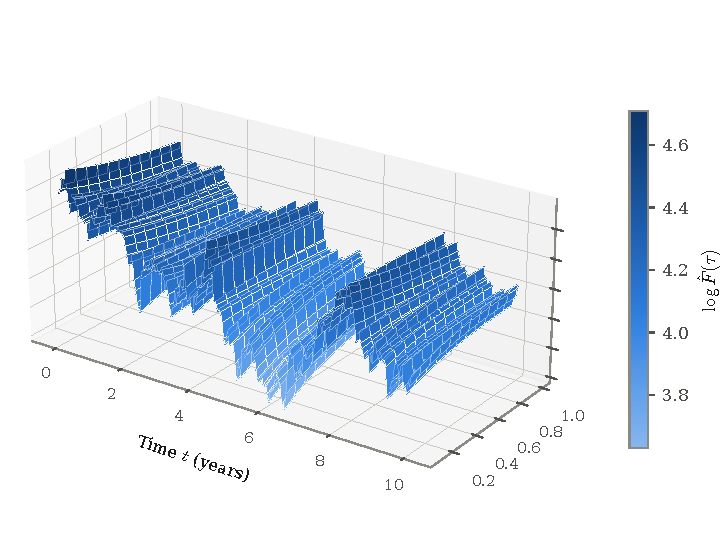
\includegraphics[height=4.5cm]{figures/methodology/mc2c_term_structure_3d.pdf}
    \subcaption{}
    \label{fig:mc_term_structure_3d}
\end{subfigure}\hfill
\begin{subfigure}[t]{0.48\textwidth}
    \centering
    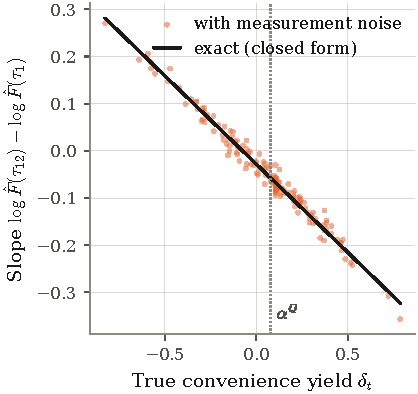
\includegraphics[height=4.5cm]{figures/results/mc3b_identifiability_scatter.pdf}
    \subcaption{}
    \label{fig:mc_identifiability_scatter}
\end{subfigure}
\caption{The simulated term structure as a 3D surface (a), showing the curve tilt through the OU cycle of $\delta_t$; and the term-structure slope as an exact affine function of $\delta$ (closed form, b), with measurement noise overlaid.}
\label{fig:mc_term_structure_and_slope}
\end{figure}

\paragraph{Evaluation Scheme.}Our evaluation spans two phases. Phase 1 validates against the known Monte Carlo ground truth $(\delta_t, S_t)$ (Equations~\ref{eq:x_discrete_em}--\ref{sde2}). Phase 2 tests out-of-sample pricing on the real WTI panel using a calendar-based holdout (Sections~\ref{sec:real_data} and~\ref{sec:holdout}). We compare six models (an MLP, AP-PEN without loss balancing, standard AP-PEN, AP-PEN (ARB), the closed-form least-squares inversion of Section~\ref{sec:ls_baseline}, and a Kalman filter baseline) across a shared metric set: state RMSE, constraint activity rate, price RMSE, benchmark correlation, and convergence diagnostics. All headline comparisons are repeated over five random seeds ($42$, $7$, $123$, $2024$, $31337$), each a full refit from scratch, and reported as mean $\pm$ standard deviation rather than from a single training run; the least-squares and Kalman baselines are deterministic given the panel and so carry no seed spread.

\paragraph{Real WTI panel.} We use dated quarterly WTI futures (Mar/Jun/Sep/Dec, Cushing delivery) instead of rolling generics to compute an exact time-to-maturity $\tau = (T-t)/365$.\footnote{Entitlement restrictions blocked chain expansion in Refinitiv Workspace~\cite{refinitiv2026eikon}, requiring individual contract queries. Archive RIC suffixes vary: single-digit year with \texttt{\^{}1} (2015--2019), single-digit year with \texttt{\^{}2} (2020--2023), and two-digit year with \texttt{\^{}2} (2024--2026).} Expiries follow the CME last-trading-day rule, perfectly matching Refinitiv's expiry field across 36 cross-validated contracts~\cite{refinitiv2026eikon}. Spot prices and financing rates come from the CLc1 continuation and FRED DGS3MO series~\cite{refinitiv2026eikon, fred2026dgs3mo}, respectively. We drop the 2020-04-20 observation because its $-\$37.63$ front-month print is a liquidation artefact, and several model constructs require $S_t > 0$.

For each date, we keep the eight nearest contracts and drop any dates that have fewer than eight. To make the data easier to process in batches, we fix the time-to-maturity ($\tau$) for each of the eight slots to its overall average, rather than tracking the exact days remaining as they shrink over time. While this makes training simpler, it does lose some temporal accuracy, which we discuss as a limitation in Section~\ref{sec:synthesis}. 

Table~\ref{tab:data_stats} shows how we filtered the raw data down to the final $2{,}770$ dates (2 January 2015 to 19 February 2026). Section~\ref{sec:real_data} visualises the term structure and market states of this final dataset.

\begin{table}[htbp]
\centering
\caption{Descriptive statistics for the real WTI futures panel}
\label{tab:data_stats}
\begin{threeparttable}
\resizebox{\textwidth}{!}{%
\begin{tabular}{lll}
\toprule
Statistic & Raw panel (Refinitiv \& FRED) & Model panel (post-construction)\tnote{a} \\
\midrule
Date range                          & 2015-01-02 -- 2026-06-29         & 2015-01-02 -- 2026-02-19 \\
Trading dates                       & $2{,}891$                        & $2{,}770$ ($95.8\%$ of dates with valid spot/rate)\tnote{b} \\
Unique contract tickers             & $52$                              & --- \\
Live contracts quoted per date      & min $6$, mode $8$, max $9$        & fixed at $8$ (ranked by $\tau$, ascending)\tnote{c} \\
Maturity slots $K$                  & ---                                & $8$ \\
Time to maturity $\tau$ (years)     & $[0.003,\ 2.00]$                  & per-slot mean $\tau \in \{0.125, 0.375, 0.625, 0.875, 1.125, 1.376, 1.626, 1.876\}$ \\
Settlement price (\$/bbl)           & $[11.57,\ 117.15]$                & $[11.57,\ 117.15]$ \\
Spot price (\$/bbl)                 & $[10.01,\ 123.70]$                & $[10.01,\ 123.70]$ \\
Risk-free rate $r$                  & $[0.000,\ 0.0563]$, mean $0.0208$ & $[0.000,\ 0.0563]$, mean $0.0208$ \\
\bottomrule
\end{tabular}%
}
\begin{tablenotes}
\footnotesize
\item[a] The model panel is the rectangular array (dates $\times$ 8 maturities) generated by \texttt{get\_data\_wti} for training (Section~\ref{sec:real_data}).
\item[b] We drop $121$ of the $2{,}891$ raw dates. One is 2020-04-20 (missing spot/rate data). The other $120$ have fewer than $8$ live contracts. Most of these ($90$) occur at the end of the sample, which is why the model panel ends early on 19 February 2026. The remaining $30$ are scattered mostly between 2015 and 2019.
\item[c] If a date has more than $8$ quoted contracts, we retain the $8$ nearest maturities. Dates with fewer than $8$ are dropped (see note b).
\end{tablenotes}
\end{threeparttable}
\end{table}


\begin{figure}[h!]
    \centering
    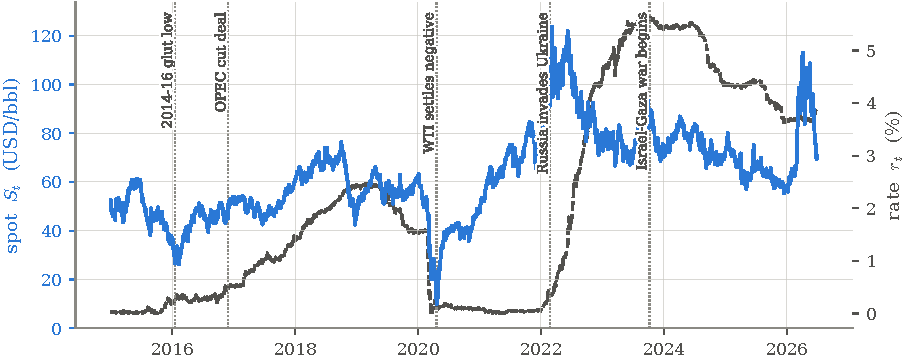
\includegraphics[width=0.8\linewidth]{figures/methodology/real_data_market_state.pdf}
    \caption{WTI spot price $S_t$ and risk-free rate $r_t$ over the sample, 2 January 2015 – 29 June 2026, with major oil-market events marked for context (2014–16 glut low, 2016 OPEC cut deal, the April 2020 negative-WTI print, Russia's invasion of Ukraine, and the start of the Israel-Gaza war).}
    \label{fig:wti_market_state}
\end{figure}



%% ════════════════════════════════════════════════════════════════════════════
%% 4. RESULTS
%% ════════════════════════════════════════════════════════════════════════════

%% ════════════════════════════════════════════════════════════════════════════
%% 4. RESULTS AND DISCUSSION
%% ════════════════════════════════════════════════════════════════════════════
%% MERGED: findings are discussed where they appear rather than deferred,
%% because the central result (constraints degrade synthetic recovery but
%% improve real recovery) cuts across the synthetic/real split and reads as a
%% contradiction if the two halves are separated.
%% BUDGET: 4.75 pp total including floats. 4.1 ~1.75, 4.2 ~1.75, 4.3 ~1.25.
%% FLOAT DISCIPLINE: aim for ~5 floats across 4.1 and 4.2 combined; 4.3 is
%% prose only. Every additional float costs roughly a third of a page of
%% argument, which is where the critical-analysis marks are.

\section{Results and Discussion}
\label{sec:results}
The evaluation proceeds in two phases. Phase 1 trains on Monte Carlo-simulated data with known Gibson--Schwartz parameters, allowing exact error measurement across four variants: an MLP, AP-PEN without loss balancing, standard AP-PEN, and AP-PEN (ARB). Phase 2 trains on real WTI futures, evaluating performance against a Kalman filter baseline since true latent states are unobservable. 

Throughout this section, we evaluate both the recovered latent state path $\hat{\delta}$ and the structural parameters $\psi$, noting that a model's accuracy in one does not guarantee success in the other.

\subsection{Synthetic Validation}
\label{sec:synthetic}
Figure~\ref{fig:path_repeat_recovery_noise_comparison} shows AP-PEN's recovery of the latent convenience yield $\delta_t$ across 20 independent simulated paths. It compares performance under baseline observation noise ($\sigma_{\text{noise}}=0.01$, panel a) to a $10\times$ higher noise level ($\sigma_{\text{noise}}=0.10$, panel b).

\begin{figure}[htbp]
    \centering
    \newlength{\prwidth}
    \setlength{\prwidth}{0.48\textwidth}
    \newlength{\prheight}
    \setlength{\prheight}{0.797\prwidth} 

    \begin{subfigure}[t]{\prwidth}
        \centering
        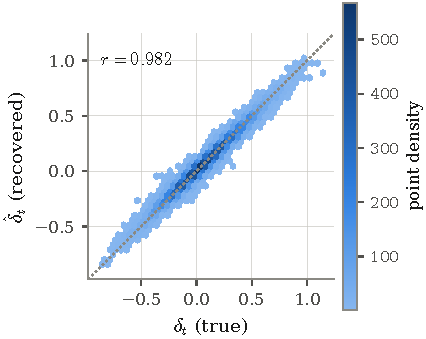
\includegraphics[width=\prwidth, height=\prheight]{figures/results/pinn3c_path_repeat_recovery.pdf}
        \subcaption{$\sigma_{\text{noise}} = 0.01$}
        \label{fig:path_repeat_recovery_noise001}
    \end{subfigure}\hfill
    \begin{subfigure}[t]{\prwidth}
        \centering
        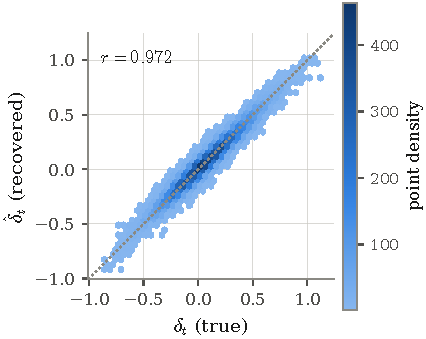
\includegraphics[width=\prwidth, height=\prheight]{figures/results/pinn3c_path_repeat_recovery_noise0.10.pdf}
        \subcaption{$\sigma_{\text{noise}} = 0.10$}
        \label{fig:path_repeat_recovery_noise010}
    \end{subfigure}

    \caption{True vs.\ recovered $\delta_t$ pooled across 20 independent paths (20{,}020 points each), shown as a hexbin density against the $y=x$ perfect-recovery line. Comparing (a) baseline to (b) $10\times$ observation noise reveals only modest degradation ($r = 0.982 \to 0.972$; RMSE = $0.050 \to 0.063$), demonstrating that AP-PEN's inversion remains robust even with significantly noisier data.}
    \label{fig:path_repeat_recovery_noise_comparison}
\end{figure}


Both figures show the model successfully recovers the latent state across both noise regimes, fulfilling our first research aim. This confirms the architecture effectively uses physical inductive biases to infer the true hidden state. Furthermore, consistent accuracy across 20 independent draws proves that this recovery is a robust, repeatable property of the method rather than an isolated success.

Looking at Figure~\ref{fig:combined_training_metrics}, we observe that some entries of $\psi$ recover well over 40k epochs, whilst others consistently diverge for each model variant. This descrepency can be attributed to the pricing transform (Eq.~\ref{eq:pricing_transform}), which can only constrain $\sigma_1$ and $\rho$ through the product $\rho\sigma_1\sigma_2$ and $\partial^2\hat F/\partial S^2 = 0$ under the affine ansatz, meaning $\sigma_1^2$ never enters the pricing transform at all.

\begin{figure}[htbp]
    \centering
    % --- Row 1: Parameters (Part 1) ---
    \begin{subfigure}[b]{0.32\textwidth}
        \centering
        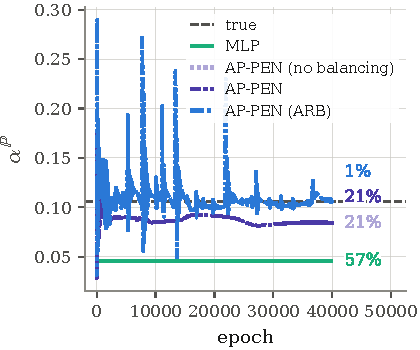
\includegraphics[width=\linewidth]{figures/results/pinn1_alphaP.pdf}
        \caption{$\alpha^{\mathbb{P}}$ recovery}
        \label{fig:pinn1_alphaP}
    \end{subfigure}\hfill
    \begin{subfigure}[b]{0.32\textwidth}
        \centering
        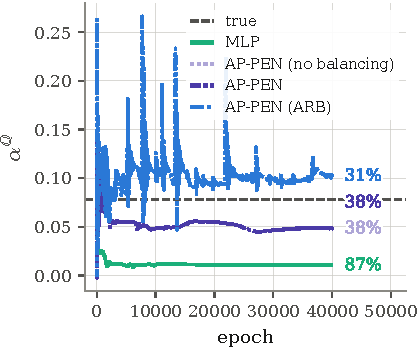
\includegraphics[width=\linewidth]{figures/results/pinn1_alphaQ.pdf}
        \caption{$\alpha^{\mathbb{Q}}$ recovery}
        \label{fig:pinn1_alphaQ}
    \end{subfigure}\hfill
    \begin{subfigure}[b]{0.32\textwidth}
        \centering
        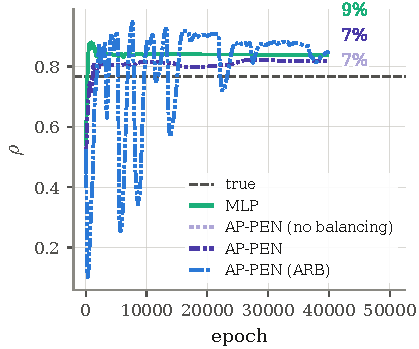
\includegraphics[width=\linewidth]{figures/results/pinn1_rho.pdf}
        \caption{$\rho$ recovery}
        \label{fig:pinn1_rho}
    \end{subfigure}
    
    \vspace{0.4cm} % Vertical spacing between rows
    
    % --- Row 2: Parameters (Part 2) ---
    \begin{subfigure}[b]{0.32\textwidth}
        \centering
        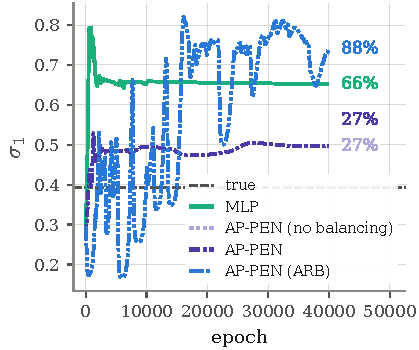
\includegraphics[width=\linewidth]{figures/results/pinn1_sigma1.pdf}
        \caption{$\sigma_1$ recovery}
        \label{fig:pinn1_sigma1}
    \end{subfigure}\hfill
    \begin{subfigure}[b]{0.32\textwidth}
        \centering
        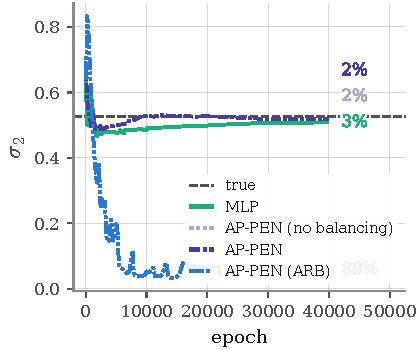
\includegraphics[width=\linewidth]{figures/results/pinn1_sigma2.pdf}
        \caption{$\sigma_2$ recovery}
        \label{fig:pinn1_sigma2}
    \end{subfigure}\hfill
    \begin{subfigure}[b]{0.32\textwidth}
        \centering
        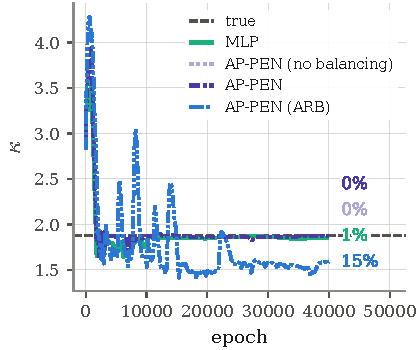
\includegraphics[width=\linewidth]{figures/results/pinn1_kappa.pdf}
        \caption{$\kappa$ recovery}
        \label{fig:pinn1_kappa}
    \end{subfigure}
    
    \vspace{0.4cm} % Vertical spacing between rows
    
    % --- Row 3: Training Losses ---
    \begin{subfigure}[b]{0.32\textwidth}
        \centering
        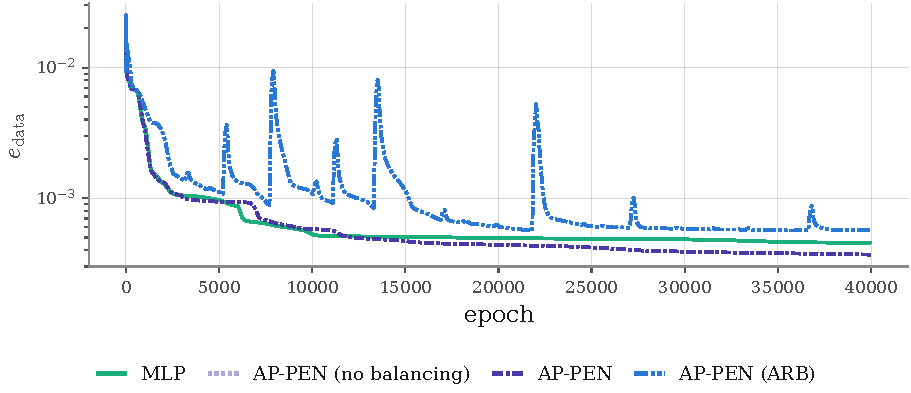
\includegraphics[width=\linewidth]{figures/results/pinn0a_training_data.pdf}
        \caption{Data misfit loss}
        \label{fig:pinn0a_training_data}
    \end{subfigure}\hfill
    \begin{subfigure}[b]{0.32\textwidth}
        \centering
        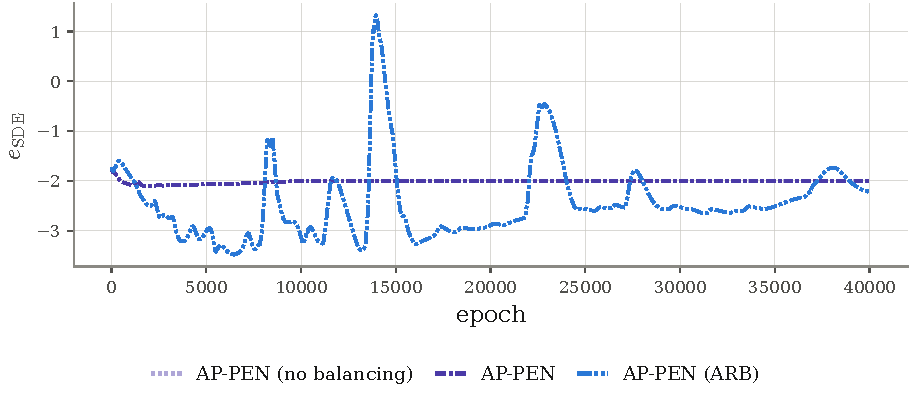
\includegraphics[width=\linewidth]{figures/results/pinn0b_training_sde.pdf}
        \caption{SDE transition NLL}
        \label{fig:pinn0b_training_sde}
    \end{subfigure}\hfill
    \begin{subfigure}[b]{0.32\textwidth}
        \centering
        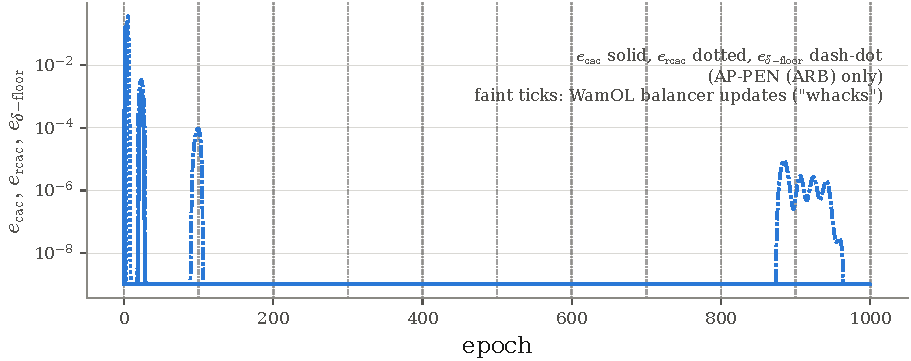
\includegraphics[width=\linewidth]{figures/results/pinn0c_training_hinges.pdf}
        \caption{Hinge losses (ARB)}
        \label{fig:pinn0c_training_hinges}
    \end{subfigure}
    
    \caption{Parameter recovery and training loss convergence across variants.}
    \label{fig:combined_training_metrics}
\end{figure}.

%   (2) PARAMETER RECOVERY. This is where the substantive finding is. Some
%       entries of $\psi$ recover tightly across draws and others do not. Give
%       your own identification argument for why: the pricing cross-section
%       constrains $\sigma_1$ and $\rho$ only through the product
%       $\rho\sigma_1\sigma_2$, and $\partial^2\hat F/\partial S^2 = 0$ under the
%       affine ansatz so $\sigma_1^2$ never enters pricing at all. If you have
%       measured the $\hat\sigma_1$--$\hat\rho$ correlation across draws, cite it;
%       if not, say the ridge is inferred from the structure of the objective
%       rather than measured, and do not overclaim.

%   (3) THE ABLATION, INCLUDING ITS NULL RESULT. AP-PEN and AP-PEN (no balancing)
%       are numerically identical. Report this as a null result and give the
%       mechanical reason: within Step 1 only the data-misfit channel carries a
%       live gradient on the path network, so the balancer has a single channel
%       to balance. Then the ARB result: path recovery barely changes while the
%       recovered $\psi$ degrades markedly. State plainly that the cash-and-carry
%       hinge is active on the unconstrained variants, meaning the simulated panel
%       itself violates the storage-cost guardrail, so the constraint is fighting
%       arbitrage-free data. Diagnose this before writing it up: it is a property
%       of the data-generating parameters, not a failure of the mechanism.}

\begin{table}[htbp]
\centering
\caption{Recovered $\psi$ on the synthetic panel (single path, seed $42$, final
epoch of 40k) against the true and initialised values, with the closed-form
profiled MLE of \S\ref{sec:ls_baseline} for reference. Rows are grouped by
whether the futures cross-section identifies the quantity
(\S\ref{sec:identifiability}); the closed-form column estimates only the
identified coordinates and so has no entry below the rule. \textsc{ap-pen} and
\textsc{ap-pen (no bal.)} are numerically identical -- the ablation's null
result (\S\ref{sec:synthetic}).}
\label{tab:synth_psi_recovery}
\begin{threeparttable}
\resizebox{\textwidth}{!}{%
\begin{tabular}{lrrrrrrr}
\toprule
Parameter & True & Init & Closed-form LS & MLP & AP-PEN (no bal.) & AP-PEN & AP-PEN (ARB) \\
\midrule
$\kappa$      & $1.8760$ & $2.8140$ & $1.8881$ & $1.8516$ & $1.8743$ & $1.8743$ & $1.5874$ \\
$\sigma_2$    & $0.5270$ & $0.6851$ & $0.5206$ & $0.5087$ & $0.5180$ & $0.5180$ & $0.0582$ \\
$m$\tnote{a}  & $0.1625$ & --- & $0.1607$ & $0.1605$ & $0.1606$ & $0.1606$ & $0.1251$ \\
\midrule
$\sigma_1$    & $0.3930$ & $0.2751$ & --- & $0.6519$ & $0.4972$ & $0.4972$ & $0.7406$ \\
$\rho$        & $0.7660$ & $0.4596$ & --- & $0.8387$ & $0.8184$ & $0.8184$ & $0.8509$ \\
$\alpha^{\mathbb{Q}}$ & $0.0779$ & $0.1379$ & --- & $0.0103$ & $0.0482$ & $0.0482$ & $0.1020$ \\
$\alpha^{\mathbb{P}}$ & $0.1060$ & $0.0460$ & --- & $0.0460$\tnote{b} & $0.0841$ & $0.0841$ & $0.1068$ \\
\midrule
$e_{\text{cac}}$ (final) & \multicolumn{3}{c}{--} & $3.31\times10^{-4}$ & $2.30\times10^{-4}$ & $2.30\times10^{-4}$ & $0.00$\tnote{c} \\
\bottomrule
\end{tabular}%
}
\begin{tablenotes}
\footnotesize
\item[a] The identified composite, $m = \alpha^{\mathbb{Q}} +
  \rho\sigma_1\sigma_2/\kappa$. Every method that fits the cross-section
  recovers it to within about $1\%$ -- including the closed form, and including
  the variants whose individual $\sigma_1$, $\rho$ and $\alpha^{\mathbb{Q}}$ are
  badly wrong. This is the row to read; the four below it are not estimable
  from a futures panel (\S\ref{sec:identifiability}) and are reported only to
  show how far apart they can drift while the price fit is unchanged.
\item[b] MLP has no $e_{\text{sde}}$ channel (no path-net-to-$\alpha^{\mathbb{P}}$
  coupling), so $\alpha^{\mathbb{P}}$ never leaves its initial value.
\item[c] The cash-and-carry hinge $e_{\text{cac}}$ is non-zero at convergence for
  every variant that does not explicitly minimise it, i.e.\ the arbitrage-free
  simulated panel itself sits outside the loose guardrail
  (\S\ref{sec:synthetic}) -- only AP-PEN (ARB), which trains against
  $e_{\text{cac}}$ directly, drives it to zero.
\end{tablenotes}
\end{threeparttable}
\end{table}

\begin{figure}[htbp]
    \centering
    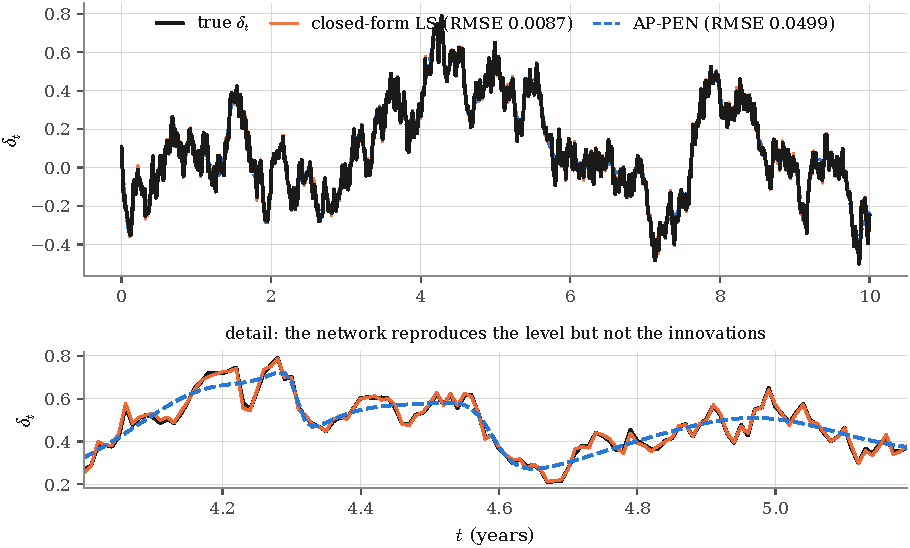
\includegraphics[width=0.92\linewidth]{figures/results/ls1_delta_recovery.pdf}
    \caption{Recovered convenience yield against the truth on the synthetic
    panel, for AP-PEN and for the closed-form least-squares inversion of
    \S\ref{sec:ls_baseline}. The upper panel covers the full ten-year path; the
    lower panel magnifies a fourteen-month window. The least-squares solution is
    visually indistinguishable from the truth, including its high-frequency
    structure, while the network traces a smooth low-frequency approximation
    that captures the level but discards the innovations. This is the same
    finding as the increment-ratio column of
    Table~\ref{tab:synth_delta_recovery}, and it localises the smoothing bias
    in the neural parameterisation rather than in the objective, since both
    estimators minimise the same log-price residual.}
    \label{fig:ls_delta_recovery}
\end{figure}

\begin{table}[htbp]
\centering
\caption{Latent-path recovery on the synthetic panel, five seeds, each a full
refit. The closed-form and no-skill rows are deterministic. ``Increment ratio''
is the standard deviation of the recovered daily increments as a fraction of
the true path's, and measures how much of the convenience yield's own dynamics
each estimator reproduces as distinct from its level.}
\label{tab:synth_delta_recovery}
\begin{threeparttable}
\resizebox{\textwidth}{!}{%
\begin{tabular}{lrrrr}
\toprule
Method & $\delta$-RMSE & Correlation & Increment ratio & Training \\
\midrule
No-skill (constant at the mean) & $0.24552$ & --- & $0\%$ & --- \\
\midrule
MLP           & $0.05093 \pm 0.00367$\tnote{b} & $0.9781 \pm 0.0032$ & $32.1 \pm 2.7\%$ & 40k epochs \\
AP-PEN        & $0.05295 \pm 0.00196$\tnote{b} & $0.9764 \pm 0.0018$ & $31.7 \pm 2.0\%$ & 40k epochs \\
AP-PEN (ARB)  & $0.06552 \pm 0.00330$ & $0.9705 \pm 0.0052$ & $24.2 \pm 2.0\%$ & 40k epochs \\
\midrule
Closed-form LS (exact MLE) & $\mathbf{0.00873}$ & $\mathbf{0.9994}$ & $\mathbf{102.8\%}$ & none\tnote{a} \\
\bottomrule
\end{tabular}%
}
\begin{tablenotes}
\footnotesize
\item[a] The per-date solve of Equation~\ref{eq:ls_delta} with $\psi$ profiled
  out: no network, no gradient steps, seconds rather than 40k epochs. It is
  $5.7\times$ more accurate than the best neural variant and, unlike any of
  them, reproduces the true increment structure essentially exactly. The neural
  estimators recover the \emph{level} of $\delta_t$ well and its
  \emph{dynamics} poorly, retaining under a third of the true innovation
  variance -- a smoothing bias attributable to the network, since the estimator
  that shares its objective but not its parameterisation does not exhibit it
  (\S\ref{sec:synthesis}).
\item[b] MLP and AP-PEN are statistically indistinguishable here: they differ
  by $0.65$ pooled standard deviations, and the ordering is the reverse of what
  a single seed ($42$) shows. This is expected rather than surprising --
  $\hat{\mathcal{L}}_{\text{SDE}}$ is stop-gradiented from the path network
  (\S\ref{sec:alternating}), so it has no route by which to improve path
  recovery, and the two variants differ only through the level of
  $\alpha^{\mathbb{Q}}$.
\end{tablenotes}
\end{threeparttable}
\end{table}

\begin{table}[htbp]
\centering
\caption{AP-PEN parameter-recovery consistency across 20 independent
Monte Carlo noise draws, each refit from scratch (path recovery: $\delta$-RMSE
mean $0.0504$, std $0.0030$ across the same 20 draws). Quantities are grouped by
whether the futures cross-section identifies them at all
(\S\ref{sec:identifiability}); the coefficient of variation makes the split
unambiguous.}
\label{tab:synth_psi_multidraw}
\begin{threeparttable}
\resizebox{0.78\textwidth}{!}{%
\begin{tabular}{llrrrr}
\toprule
& Quantity & True & Mean recovered & Std across draws & CV \\
\midrule
\multirow{3}{*}{\rotatebox{90}{\footnotesize Identified}}
& $\kappa$      & $1.8760$ & $1.8476$ & $0.0242$ & $1.3\%$ \\
& $\sigma_2$    & $0.5270$ & $0.5425$ & $0.0489$ & $9.0\%$\tnote{a} \\
& $m = \alpha^{\mathbb{Q}} + \rho\sigma_1\sigma_2/\kappa$ & $0.1625$ & $0.1654$ & $0.0063$ & $\mathbf{3.8\%}$ \\
\midrule
\multirow{4}{*}{\rotatebox{90}{\footnotesize Unidentified}}
& $\sigma_1$    & $0.3930$ & $0.5511$ & $0.2725$ & $49.4\%$\tnote{b} \\
& $\rho$        & $0.7660$ & $0.7002$ & $0.3577$ & $51.1\%$\tnote{b} \\
& $\rho\sigma_1\sigma_2$ & $0.1586$ & $0.2424$ & $0.1712$ & $\mathbf{70.6\%}$\tnote{b} \\
& $\alpha^{\mathbb{Q}}$ & $0.0779$ & $0.0346$ & $0.0917$ & $265\%$\tnote{b} \\
\midrule
& $\alpha^{\mathbb{P}}$ & $0.1060$ & $0.0728$ & $0.0919$ & $126\%$\tnote{c} \\
\bottomrule
\end{tabular}%
}
\begin{tablenotes}
\footnotesize
\item[a] $\sigma_2$ is identified, but only weakly: it enters $A(\tau)$ through
  the $(1-e^{-2\kappa\tau})$ basis function alone, which is close to collinear
  with the other two at short maturities. It is correspondingly the first
  quantity to degrade under observation noise (\S\ref{sec:synthetic}).
\item[b] These are the flat directions of \S\ref{sec:identifiability}. The
  spread is not estimation error in the usual sense: pinning any of them leaves
  every $(\kappa, \sigma_2, m)$ reachable, so the objective is exactly
  indifferent and the recovered value reflects only the initialisation and the
  optimiser's trajectory. Note that the confounding extends past the familiar
  $\rho\sigma_1\sigma_2$ product: the product itself is not identified either,
  being separable from $\alpha^{\mathbb{Q}}$ only through $m$.
\item[c] $\alpha^{\mathbb{P}}$ is identified in principle, but only through the
  transition channel $\hat{\mathcal{L}}_{\text{SDE}}$ acting on an already
  heavily smoothed path, which carries little information about the
  mean-reversion level over a ten-year sample.
\end{tablenotes}
\end{threeparttable}
\end{table}

\subsection{Real WTI Application}
\label{sec:real_data}

\begin{figure}[h!]
    \centering
    \begin{subfigure}{\textwidth}
        \centering
        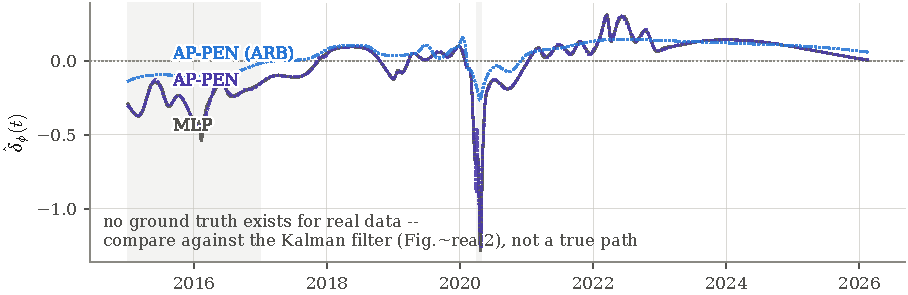
\includegraphics[width=0.8\linewidth]{figures/results/real1_pinn_recovery.pdf}
        \caption{Recovered $\hat{\delta}_\phi(t)$ for the three real-data variants. No ground truth exists here: $\delta_t$ is latent by construction, so these paths can only be assessed against each other, against the benchmark in (b), and against economic plausibility. Note the April 2020 excursion in the two unconstrained variants.}
        \label{fig:real1_pinn_recovery}
    \end{subfigure}
    
    \vspace{0.5cm} % Adjust this to change spacing between the figures
    
    \begin{subfigure}{\textwidth}
        \centering
        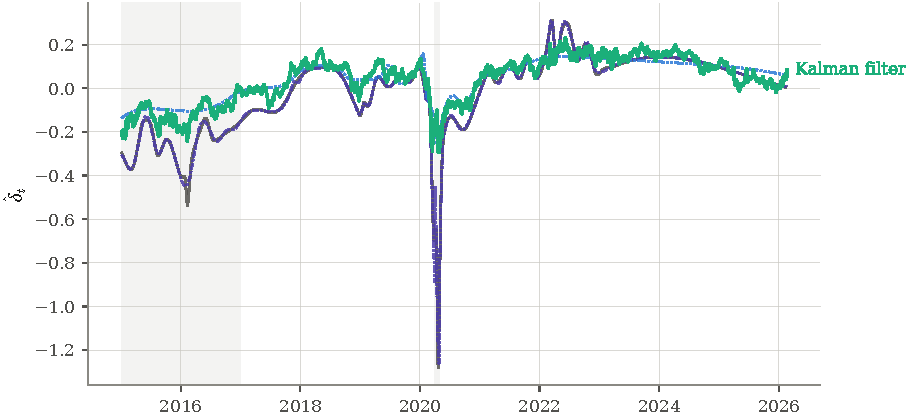
\includegraphics[width=0.8\linewidth]{figures/results/real2_pinn_vs_kalman.pdf}
        \caption{The same three variants overlaid on the Kalman filter's own filtered $\hat{\delta}_t$, on their common dates. The Kalman path is a benchmark, not ground truth: it is an independent estimate carrying its own state-transition prior, which is what suppresses the April 2020 excursion visible in (a).}
        \label{fig:real2_pinn_vs_kalman}
    \end{subfigure}
    
    \caption{Convenience yield recovered from the real WTI panel (2015--2026), shown in isolation (a) and against the Kalman filter benchmark (b). The two unconstrained variants track each other almost exactly but breach $-1.2$ during the April 2020 dislocation; AP-PEN (ARB), whose hinge penalties are active, stays within its guardrails throughout. Section~\ref{sec:real_data} argues that this range comparison, rather than the correlation against the benchmark, is the informative one.}
    \label{fig:real_results_combined}
\end{figure}


% \todo{BUDGET ~1.75 pp including floats. Three paragraphs.

%   (1) THE BASELINE. Two or three sentences only; panel construction now sits in
%       \S\ref{sec:experimental_design}. State that the filter converges, give its
%       in-sample fit quality and the distributional summary of its recovered
%       $\hat\delta_t$ in prose. Do not spend a float on three numbers.

%   (2) THE COMPARISON. Correlation and RMSE of each variant against the Kalman
%       baseline on the common dates. The decisive evidence here is the recovered
%       range rather than the correlation: the unconstrained variants produce
%       convenience-yield excursions far below any economically defensible level,
%       and the constrained variant does not. Make the argument that the
%       constraints are doing real work on real data in a way they were not on
%       synthetic data.

%   (3) THE PARAMETER PATHOLOGY. Do not bury this. The best-performing variant on
%       path agreement recovers structurally implausible dynamics: mean reversion
%       effectively switched off, a sign-flipped correlation against every
%       published estimate, and a long-run convenience yield orders of magnitude
%       outside any observed range. State what this means -- the constrained model
%       is buying path plausibility with meaningless dynamics. Compare the Kalman
%       filter's own recovered parameters as a reference point, and note any
%       finding common to all methods (for instance the sign of
%       $\alpha^{\mathbb Q}$) against the sample's backwardation frequency.

%   Optionally close with one or two sentences of economic reading (the crisis
%   windows already identified in the constraint mechanism, backwardation and
%   contango regimes) but only if the recovered path visibly supports it. Do not
%   speculate to fill space.}

\begin{table}[htbp]
\centering
\caption{Recovered $\hat\delta_t$ against the Kalman filter benchmark on real
WTI, common dates (2015-01-05 to 2026-02-19). Correlation/RMSE are against the
Kalman filtered path; range/mean/std describe each method's own recovered
series in isolation.}
\label{tab:real_kalman_comparison}
\begin{threeparttable}
\resizebox{\textwidth}{!}{%
\begin{tabular}{lrrrrr}
\toprule
Method & corr.\ vs.\ KF & RMSE vs.\ KF & $\hat\delta_t$ range & mean & std \\
\midrule
Kalman filter (reference) & -- & -- & $[-0.293,\ 0.232]$ & $0.040$ & $0.108$ \\
\midrule
Constant at the KF mean (null)\tnote{a} & -- & $0.108$ & -- & $0.040$ & $0$ \\
\midrule
Closed-form LS (exact MLE)\tnote{b} & $0.922$ & $0.112$ & $[-1.654,\ 0.421]$ & $-0.018$ & $0.187$ \\
MLP           & $0.9176 \pm 0.0012$ & $0.1089 \pm 0.0004$\tnote{c} & $[-1.282,\ 0.312]$\tnote{d} & $-0.018$ & $0.181$ \\
AP-PEN        & $0.9170 \pm 0.0010$ & $0.1089 \pm 0.0004$\tnote{c} & $[-1.263,\ 0.312]$\tnote{d} & $-0.017$ & $0.182$ \\
AP-PEN (ARB)  & $\mathbf{0.9469 \pm 0.0034}$ & $\mathbf{0.0348 \pm 0.0010}$ & $[-0.300,\ 0.158]$\tnote{e} & $0.045$ & $0.088$ \\
\bottomrule
\end{tabular}%
}
\begin{tablenotes}
\footnotesize
\item[a] A constant series fixed at the Kalman filter's own sample mean. Its
  RMSE against the filter is by construction the filter's own standard
  deviation, $0.108$. Every cross-sectional method in this table scores at or
  above that figure, so on this metric none of them beats predicting a
  constant. Reporting it is what makes the correlation column interpretable:
  correlations near $0.92$ look strong but are scale-free and do not penalise
  the amplitude disagreement that drives the RMSE.
\item[b] The closed-form profiled MLE of \S\ref{sec:ls_baseline} -- the exact
  maximum-likelihood solution of the same model, with no network and no
  training. It disagrees with the Kalman filter by \emph{more} than any neural
  variant. This is the decisive observation for interpreting this table: the
  disagreement is not a deficiency of the network but a systematic difference
  between cross-sectional inversion and state-space filtering. Pairwise, the
  three cross-sectional estimators agree with each other to within $0.014$--$0.033$
  and each differs from the filter by $\approx0.11$; it is the benchmark that
  sits apart.
\item[c] Neural rows are mean $\pm$ standard deviation over five seeds. The
  spread is small enough to settle the comparison: MLP and AP-PEN are
  \emph{statistically indistinguishable} here (their correlations differ by
  $0.0006$ against a seed standard deviation of $0.001$, and their RMSEs agree
  to four decimal places), which is what the architecture predicts, since the
  two variants differ only through the level of $\alpha^{\mathbb{Q}}$
  (\S\ref{sec:alternating}). It also confirms that both sitting above the null
  is a stable property rather than an unlucky draw.
\item[d] MLP/AP-PEN breach $-1.28$/$-1.26$, far outside any economically
  defensible convenience yield, and AP-PEN (ARB) does not. The excursions fall
  on the April 2020 dislocation. Note however that the exact MLE breaches
  $-1.65$ on the same dates: this is what the Gibson--Schwartz model implies
  from the observed curve, not an artefact of neural training, so the
  constraint should be read as imposing prior economic information the data
  does not contain rather than as repairing an estimation failure
  (\S\ref{sec:synthesis}).
\item[e] The lower end is $-0.300$ on every seed, i.e.\ exactly the
  $\delta_{\min}$ guardrail of \S\ref{sec:constraints}. AP-PEN (ARB) is not
  finding an economically plausible path so much as being clamped to the
  boundary of the admissible region, which is the same reading as the
  $\kappa$-floor behaviour in Table~\ref{tab:real_psi_pathology}.
\end{tablenotes}
\end{threeparttable}
\end{table}

\begin{table}[htbp]
\centering
\caption{Recovered structural parameters $\psi$ on real WTI, by method. Kalman
values are the full-sample MLE fit (\S\ref{sec:kalman}); the closed-form column
is the profiled MLE of \S\ref{sec:ls_baseline}, which estimates the identified
coordinates directly and so has no entry for the flat directions. AP-PEN
columns are the converged $\psi$ from the corresponding 40k-epoch calibration,
shown both without the $\kappa$ floor (as originally run) and with
$\kappa_{\min}=0.1$ imposed (\S\ref{sec:pinn_inversion}). Only the top block is
estimable from a futures panel; the middle block is reported for completeness
but is not identified (\S\ref{sec:identifiability}).}
\label{tab:real_psi_pathology}
\begin{threeparttable}
\resizebox{\textwidth}{!}{%
\begin{tabular}{lrrrrrr}
\toprule
& & & \multicolumn{2}{c}{Unfloored} & \multicolumn{2}{c}{$\kappa_{\min}=0.1$} \\
\cmidrule(lr){4-5}\cmidrule(lr){6-7}
Parameter & Kalman (MLE) & Closed-form LS & AP-PEN & AP-PEN (ARB) & AP-PEN & AP-PEN (ARB) \\
\midrule
$\kappa$      & $0.4257$ & $0.9512$ & $0.9301$ & $0.0028$\tnote{a} & $0.9234$ & $0.1002$\tnote{b} \\
$\sigma_2$    & $0.1726$ & $0.5516$ & $0.5444$ & $0.0557$ & $0.5449$ & $0.0481$ \\
$m$\tnote{c}  & $0.0811$ & $0.1871$ & $0.1888$ & $-4.5436$ & $0.1908$ & $-0.0206$ \\
\midrule
$\sigma_1$    & $0.4397$ & --- & $0.7660$ & $0.0051$ & $0.7680$ & $0.0031$ \\
$\rho$        & $0.8883$ & --- & $0.9676$ & $-0.8198$\tnote{d} & $0.9674$ & $-0.0188$ \\
$\alpha^{\mathbb{Q}}$ & $-0.0773$ & --- & $-0.2450$ & $-4.4599$ & $-0.2477$ & $-0.0206$ \\
$\alpha^{\mathbb{P}}$ & $0.1007$ & --- & $0.0120$ & $4.3741$ & $0.0114$ & $0.1900$ \\
\bottomrule
\end{tabular}%
}
\begin{tablenotes}
\footnotesize
\item[a] Mean reversion effectively switched off. This is not a random failure
  but the $1/\kappa$ pole of \S\ref{sec:pinn_inversion} being exploited: with
  $\alpha^{\mathbb{Q}}$ derived rather than free, driving $\kappa\to0$ is the
  only lever the pricing channel has on its level, and it buys
  $\sigma_2\lambda_2/\kappa = 8.83$ at negligible cost to the fit. At this
  $\kappa$, $B(\tau)\to-\tau$ and the two-factor model has degenerated into a
  deterministic cost-of-carry curve.
\item[b] With the floor imposed, AP-PEN (ARB) converges \emph{exactly onto it},
  and does so on all five seeds ($\kappa = 0.100 \pm 0.000$). The floor
  therefore bounds the pathology without curing it: the constrained objective
  still pulls the solution to a degenerate corner, and $\sigma_1$ collapses to
  $0.003$ regardless. That the behaviour is identical across every
  initialisation rules out a stochastic optimisation failure -- the hinge
  penalties, not the parameterisation or the seed, are what drive the
  degeneracy.
\item[c] $m = \alpha^{\mathbb{Q}} + \rho\sigma_1\sigma_2/\kappa$, the only
  combination of the lower block the futures cross-section can determine
  (\S\ref{sec:identifiability}). Note the agreement between AP-PEN and the
  closed-form MLE ($0.189$ vs.\ $0.187$) against the Kalman filter's $0.081$:
  the two cross-sectional estimators concur, and it is the state-space
  benchmark that differs.
\item[d] Sign-flipped against every other method here and against published
  GS estimates (all $\rho>0$) -- but see \S\ref{sec:identifiability}: $\rho$ is
  not identified from prices, so no weight should be placed on its sign in any
  of the AP-PEN columns.
\end{tablenotes}
\end{threeparttable}
\end{table}

\begin{figure}[htbp]
    \centering
    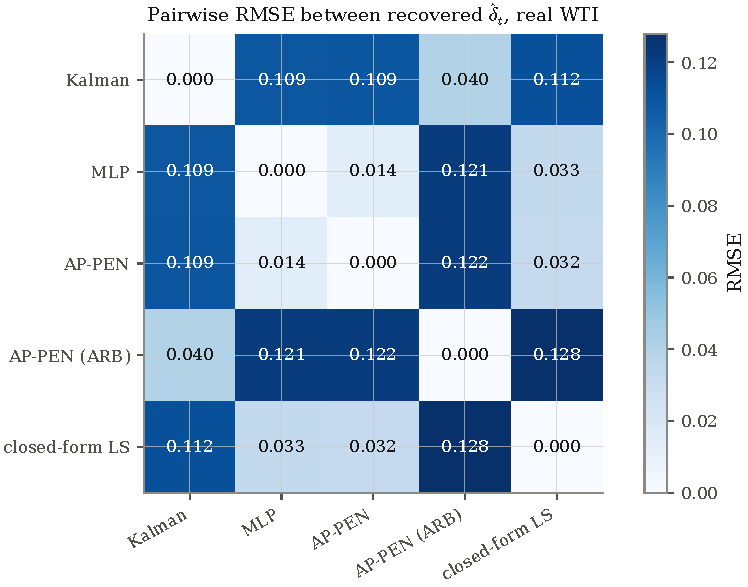
\includegraphics[width=0.68\linewidth]{figures/results/ls2_agreement_matrix.pdf}
    \caption{Pairwise RMSE between the convenience-yield paths recovered by
    each method on the real WTI panel, over their common dates. The three
    cross-sectional estimators --- both neural variants and the closed-form
    maximum-likelihood solution --- agree with one another to within $0.014$ to
    $0.033$, while each differs from the Kalman filter by approximately
    $0.11$. Since one of the three is the exact MLE of the same model, the
    disagreement cannot be read as a deficiency of the network: what separates
    the estimators is whether $\delta_t$ is inferred from the cross-section of
    prices at each date or from a state equation propagated through time.
    AP-PEN (ARB) is the exception in the opposite direction, agreeing with the
    filter ($0.040$) while disagreeing with the estimator it is closest to in
    construction ($0.128$) --- the signature of a path constrained toward a
    narrow band rather than one recovered from the data
    (\S\ref{sec:real_data}).}
    \label{fig:agreement_matrix}
\end{figure}

\subsubsection{Constraint Activity: Do the Hinges Do Anything?}
\label{sec:constraint_activity}

The tables above report what the hinge terms \emph{cost}. The metric that
reports what they \emph{buy} is the constraint activity rate promised in
\S\ref{sec:experimental_design}, given in Table~\ref{tab:constraint_activity}.
It is measured on the $(\text{date} \times \text{maturity})$ grid for the two
price bounds and on the date axis for the convenience-yield floor, and the
first row of each panel is model-free: it references only
$(F^{\text{obs}}, S_t, \tau, r_t)$ and so establishes whether a constraint has
anything to bind against before any model is fitted.

\begin{table}[htbp]
\centering
\caption{Constraint activity rates. The observed row is model-free and sets the
baseline; a hinge can only do work where the data itself violates the bound.
Percentages are of the full grid ($22{,}160$ points on the real panel,
$12{,}012$ on the synthetic), except the final column which is a percentage of
dates.}
\label{tab:constraint_activity}
\begin{threeparttable}
\resizebox{0.92\textwidth}{!}{%
\begin{tabular}{llrrr}
\toprule
Panel & Series & cac violated & rcac violated\tnote{a} & $\hat\delta < \delta_{\min}$ \\
\midrule
\multirow{4}{*}{Real WTI}
& Observed panel (model-free)\tnote{b} & $1.84\%$ & $0.00\%$ & --- \\
& MLP (no hinges)                      & $1.98\%$ & $0.00\%$ & $7.44\%$ \\
& AP-PEN (no hinges)                   & $2.00\%$ & $0.00\%$ & $6.90\%$ \\
& \textbf{AP-PEN (ARB), hinges on}     & $\mathbf{0.00\%}$ & $0.00\%$ & $\mathbf{0.69\%}$ \\
\midrule
\multirow{4}{*}{Synthetic}
& Observed panel (model-free)          & $0.70\%$ & $0.03\%$ & $4.30\%$\tnote{c} \\
& MLP (no hinges)                      & $0.36\%$ & $0.00\%$ & $3.30\%$ \\
& AP-PEN (no hinges)                   & $0.32\%$ & $0.00\%$ & $3.50\%$ \\
& AP-PEN (ARB), hinges on              & $0.00\%$ & $0.00\%$ & $0.20\%$\tnote{c} \\
\bottomrule
\end{tabular}%
}
\begin{tablenotes}
\footnotesize
\item[a] The reverse cash-and-carry floor is essentially never active anywhere:
  $\delta_{\max}=0.75$ is a genuine outer guardrail that never binds in either
  panel. It is retained for completeness of the no-arbitrage pair, but no claim
  rests on it, and this is worth stating rather than leaving the reader to
  infer that all three hinges contribute equally.
\item[b] The observed WTI panel violates the cash-and-carry ceiling on $1.84\%$
  of points, falling on $135$ dates concentrated entirely in 2015 ($42$), 2016
  ($55$) and 2020 ($38$) --- the shale-glut contango and the April 2020
  storage-exhaustion episode. The unconstrained variants inherit and very
  slightly amplify this ($1.98$--$2.00\%$), which is the correct behaviour for
  an estimator fitting the data faithfully. AP-PEN (ARB) eliminates it
  entirely, and reduces implausible convenience-yield states by an order of
  magnitude ($7.4\% \to 0.7\%$).
\item[c] The same mechanism runs in reverse on simulated data, and this is what
  resolves the apparent contradiction between the two panels. The
  \emph{true} $\delta_t$ of the data-generating process lies below
  $\delta_{\min}$ on $4.30\%$ of dates; the unconstrained variants track that
  faithfully ($3.3$--$3.5\%$), and AP-PEN (ARB) suppresses it to $0.20\%$. On
  the synthetic panel the hinge is therefore not correcting an error --- it is
  penalising states the process genuinely visits, which is precisely why it
  degrades recovery there (Table~\ref{tab:synth_delta_recovery}) while
  improving it on real data.
\end{tablenotes}
\end{threeparttable}
\end{table}

\noindent
Three conclusions follow, and together they are the substantive result on the
constraint mechanism. First, \textbf{the hinges bind and they work}: on the
real panel the cash-and-carry violation rate goes to exactly zero from a
model-free baseline of $1.84\%$, and the fraction of dates on which the
recovered convenience yield falls below any defensible floor drops by an order
of magnitude. This is the DC-PINN inequality mechanism transferred to
commodity-specific economics and doing exactly what it was designed to do.
Second, \textbf{they are not free}, and the price is now quantified in three
separate places: a threefold in-sample price-fit penalty
(Table~\ref{tab:holdout}), a degenerate $\psi$ that a $\kappa$ floor bounds but
does not cure (Table~\ref{tab:real_psi_pathology}), and worse latent-state
recovery wherever the bounds are not the binding economics
(Table~\ref{tab:synth_delta_recovery}). Third, and most usefully for anyone
adopting the mechanism, \textbf{whether it helps is decided by the observed
violation rate, not by the model}: the constraint earns its cost exactly where
the data violates it and not otherwise, and that rate is measurable in advance
of any fitting, from $(F^{\text{obs}}, S_t, \tau, r_t)$ alone.

\medskip
\noindent\emph{Note for the prose:} $\alpha^{\mathbb{Q}}$ is negative under
\emph{every} method above, including the Kalman filter -- a finding common
across estimation approaches. The real WTI sample is in backwardation
(near-term settle above the longest-dated slot) on $64.2\%$ of the $2{,}770$
trading dates, consistent with $\delta_t$ typically sitting above a low/negative
$\alpha^{\mathbb{Q}}$.



\subsection{Temporal Holdout}
\label{sec:holdout}

This is not a classical train/test split: $\delta_t$ is latent, so there is
nothing to hold out and score against directly. What is tested instead is
whether $\psi$ and the path network, fitted on dates before 2024-01-01, still
price \emph{observed} futures on the $533$ later dates ($19.2\%$ of the panel)
the model never saw. It also stress-tests a structural limitation of the
architecture: $\hat{\delta}_\phi$ is a plain function of normalised calendar
time, so every test date lies outside its trained domain and is reached by
neural extrapolation.

\begin{table}[htbp]
\centering
\caption{Out-of-sample pricing on the real WTI panel, train $<$2024 / test
$\geq$2024. Log-price RMSE, reported as mean $\pm$ standard deviation over five
seeds, each a full refit. The two closed-form rows are deterministic and bracket
what is achievable.}
\label{tab:holdout}
\begin{threeparttable}
\resizebox{\textwidth}{!}{%
\begin{tabular}{lrrr}
\toprule
Method & In-sample RMSE & Out-of-sample RMSE & Ratio (range over seeds) \\
\midrule
Kalman filter, filtered through the test window\tnote{a} & $0.02802$ & $0.01638$ & $0.58\times$ \\
\textbf{Kalman filter, forecast only}\tnote{b} & $0.02802$ & $0.03007$ & $\mathbf{1.07\times}$ \\
\midrule
Closed-form LS, $\delta_t$ re-solved per test date\tnote{c} & $0.01424$ & $0.00984$ & $0.69\times$ \\
Closed-form LS, $\delta_t$ frozen at last trained value\tnote{d} & $0.01424$ & $0.03869$ & $2.72\times$ \\
\midrule
MLP           & $0.02486 \pm 0.00118$ & $0.14581 \pm 0.17861$ & $5.73\times \pm 6.81$ \ \ [$1.50$--$19.24$]\tnote{e} \\
AP-PEN        & $0.02429 \pm 0.00129$ & $0.16609 \pm 0.12409$ & $6.71\times \pm 4.83$ \ \ [$1.80$--$14.70$]\tnote{e} \\
AP-PEN (ARB)  & $0.07181 \pm 0.03624$ & $\mathbf{0.05517 \pm 0.00691}$ & $\mathbf{0.93\times \pm 0.33}$ \ \ [$0.42$--$1.26$] \\
\bottomrule
\end{tabular}%
}
\begin{tablenotes}
\footnotesize
\item[a] The filter refitted by maximum likelihood on the training window alone
  (\S\ref{sec:kalman}), then run forward through the test window updating on
  each test observation in turn. This is the filter's own natural out-of-sample
  metric and an upper bound on what it can do, but it is \emph{not} comparable
  to the neural rows, since it keeps reading the data it is being scored on. It
  is reported because the gap to (b) measures how much of the filter's
  advantage comes from that privilege.
\item[b] \textbf{The like-for-like comparator.} Same train-window $\psi$ and the
  filtered state at the cutoff, with $\delta_t$ then propagated forward by the
  transition mean alone and \emph{no} measurement updates; the observed spot is
  used, exactly as the neural models use it, so only the latent state is
  forecast. This is the same information set the path network has, and the
  incumbent degrades by $7\%$ where the unconstrained neural variants degrade by
  factors of five to seven. The forecast is also economically meaningful:
  $\hat\delta$ decays from $+0.146$ at the cutoff to $+0.084$ two years later,
  reverting toward its fitted $\alpha^{\mathbb{P}} = 0.044$. A state equation
  extrapolates; a network of calendar time saturates.
\item[c] $\psi$ fitted on the training window, then $\delta_t$ solved in closed
  form at each test date from that date's own prices. This isolates
  generalisation of $\psi$ alone and is the achievable floor; like (a) it is not
  directly comparable to the neural rows. The ratio falls below one because
  2024--26 is a calmer, more consistently backwardated window than the training
  period.
\item[d] The same $\psi$, with $\delta_t$ held at its final in-sample value
  throughout the test window --- the cost of not extrapolating at all.
\item[e] \emph{The single-seed result does not survive replication.} On seed
  $42$ alone these read $8.86\times$ and $1.69\times$ respectively, which would
  support the claim that the transition channel buys out-of-sample robustness.
  Over five seeds the ordering reverses in the mean and the per-seed spreads
  overlap almost entirely, so no such advantage is demonstrable: the apparent
  effect was sampling variation in the network initialisation. This is
  consistent with the architecture, since $\hat{\mathcal{L}}_{\text{SDE}}$ is
  stop-gradiented from the path network and therefore cannot regularise the
  extrapolation directly (\S\ref{sec:alternating}); the two variants differ only
  through the level of $\alpha^{\mathbb{Q}}$.
\end{tablenotes}
\end{threeparttable}
\end{table}

\noindent
Read against the incumbent, the ordering is unflattering. The Kalman filter,
refitted on the same training window and given exactly the same information the
path network has, degrades by $1.07\times$; the unconstrained neural variants
degrade by factors of five to seven. Only AP-PEN (ARB) is competitive
($0.93\times$), and it achieves that not by forecasting but by being bounded:
the hinge penalties clamp the recovered path, so when the network extrapolates
past its trained domain it cannot run away. It pays roughly three times the
in-sample price error for that stability. The unconstrained variants are
individually capable of extrapolating well --- both achieve ratios below
$2\times$ on some seeds --- but not dependably, and a practitioner cannot know
in advance which seed they have drawn.

The distinction that matters is between bounding an extrapolation and
performing one. The filter propagates a state equation, so its
$\hat\delta$ reverts toward $\alpha^{\mathbb{P}}$ at the fitted rate and
carries genuine information about the held-out window; AP-PEN (ARB) merely
fails to move far. That difference is invisible in a price-RMSE column and
becomes explicit in the next table, where the latent state itself is scored.

Price reconstruction is, however, only a proxy for what the holdout is meant to
test. The same split can be run on the synthetic panel, where $\delta_t$ is
known over the whole domain including the held-out window, and the latent state
can therefore be scored directly rather than inferred from price fit.
Table~\ref{tab:mc_holdout} does so, and the result is considerably harsher than
the price-based view suggests.

\begin{table}[htbp]
\centering
\caption{Synthetic temporal holdout: train on $t \leq 8$yr, test on the final
two years ($20.1\%$ of the path), five seeds. Unlike
Table~\ref{tab:holdout}, the held-out latent state is known, so out-of-sample
$\delta$ error is measured rather than proxied.}
\label{tab:mc_holdout}
\begin{threeparttable}
\resizebox{\textwidth}{!}{%
\begin{tabular}{lrrrr}
\toprule
Variant & $\delta$-RMSE in & $\delta$-RMSE out & vs.\ no-skill\tnote{a} & Out-of-sample correlation \\
\midrule
No-skill (constant on test window) & --- & $0.20788$ & $1.00\times$ & --- \\
\midrule
MLP           & $0.04737 \pm 0.00131$ & $0.41137 \pm 0.14761$ & $1.98\times$ & $+0.564 \pm 0.314$\tnote{b} \\
AP-PEN        & $0.04868 \pm 0.00188$ & $0.29669 \pm 0.15342$ & $1.43\times$ & $+0.718 \pm 0.072$ \\
AP-PEN (ARB)  & $0.06073 \pm 0.00289$ & $0.52459 \pm 0.15618$ & $2.52\times$ & $-0.410 \pm 0.592$\tnote{b} \\
\bottomrule
\end{tabular}%
}
\begin{tablenotes}
\footnotesize
\item[a] Out-of-sample $\delta$-RMSE as a multiple of the no-skill baseline,
  i.e.\ of simply predicting a constant equal to the test window's mean.
  \textbf{Every variant exceeds one.} In-sample each recovers the path to
  roughly $0.05$, a fifth of the no-skill level; extrapolated two years past
  the training cutoff, all three are between $1.4$ and $2.5$ times
  \emph{worse} than a constant. The degradation from in- to out-of-sample is a
  factor of six to nine.
\item[b] The out-of-sample correlations are not merely weak but unstable in
  sign across seeds: MLP ranges from $-0.05$ to $+0.80$ and AP-PEN (ARB) from
  $-0.81$ to $+0.77$. An estimator whose recovered path may correlate either
  positively or negatively with the truth depending on initialisation is
  carrying no usable information about the held-out window.
\end{tablenotes}
\end{threeparttable}
\end{table}

\noindent
This is the clearest statement of the architecture's central limitation, and it
follows directly from the design rather than from any tuning choice.
$\hat{\delta}_\phi$ is a function of normalised calendar time alone; past the
training cutoff a $\tanh$ network saturates toward a constant bearing no
relation to the true path, and nothing in the objective supplies the dynamics
that would let it do otherwise --- $\hat{\mathcal{L}}_{\text{SDE}}$, the one
channel encoding the $\mathbb{P}$-dynamics, is stop-gradiented away from the
path network (\S\ref{sec:alternating}). The model interpolates the latent state
well and does not extrapolate it at all.

Note also that AP-PEN (ARB)'s protective behaviour in
Table~\ref{tab:holdout} does not reappear here: it is the worst variant on this
split ($8.88\times$ price ratio, $2.52\times$ no-skill on $\delta$). The
explanation is the same one \S\ref{sec:synthetic} gives for the constraints
hurting on simulated data --- on the synthetic panel the guardrails sit well
outside the realised range of $\delta_t$ and never bind, so they cannot bound
the extrapolation the way they do on the real panel. The stability observed in
Table~\ref{tab:holdout} is therefore a property of the constraints binding
against real prices, not a general property of the constrained variant.

\subsection{Synthesis and Limitations}
\label{sec:synthesis}

% \todo{BUDGET ~1.25 pp, prose only, no floats. This subsection carries most of
%   the critical-analysis marks. Four paragraphs.

%   (1) THE CENTRAL CONTRADICTION, RESOLVED. Constraints hurt on synthetic data
%       and help on real data. Your explanation must reconcile both: the synthetic
%       panel is generated from an arbitrage-free model whose parameters happen to
%       violate a loose guardrail, so the hinge fights correct data.
%       REVISED after the closed-form baseline was run: do NOT write the second
%       half as "the real panel contains genuine pathologies the unconstrained
%       model fits happily." The exact MLE (\S\ref{sec:ls_baseline}) reaches
%       $-1.65$ on the same April 2020 dates, so the excursion is what
%       Gibson--Schwartz implies from the observed curve, not something the
%       unconstrained network invents. The honest framing is that the constraint
%       injects prior economic information the data does not contain -- it is
%       overriding the model, not repairing an estimation failure. That is still
%       a defensible thing to do; it just is not "the constraint finds the right
%       answer." State what this implies about when soft economic constraints are
%       worth their cost, and note the price: on real data the constrained variant
%       buys its path plausibility with a degenerate $\psi$
%       (Table~\ref{tab:real_psi_pathology}) that a $\kappa$ floor bounds but does
%       not cure.

%   (2) PATH RECOVERY IS NOT PARAMETER RECOVERY. This holds on both datasets and is
%       the thesis's most transferable claim. Explain why a model can track
%       $\hat\delta(t)$ closely while $\psi$ is structurally wrong, and what that
%       means for anyone reading economic quantities off the parameters rather than
%       the path.

%   (3) AGAINST THE KALMAN BASELINE. When does AP-PEN beat it and when not? Address
%       the smoother-versus-filter asymmetry head-on (\S\ref{sec:kalman}):
%       $\hat\delta_\phi$ is fitted over the whole sample and so uses future
%       information, which the causal filter does not, so any accuracy advantage is
%       partly attributable to that rather than to architecture. The closed-form
%       per-date baseline HAS now been run (\S\ref{sec:ls_baseline}) -- do not
%       write that it was not. Report it honestly: on synthetic data it beats
%       every neural variant outright, and on real data all three cross-sectional
%       estimators agree with each other far more closely than any of them agrees
%       with the filter. That reframes the benchmark comparison from "is AP-PEN
%       accurate?" to "cross-section versus state space," which is the more
%       defensible question given no ground truth exists.

%   (4) LIMITATIONS, as one dense paragraph or a tight list. Cover: no
%       differential-equation residual remains, so the physics is imposed by
%       construction rather than learned (defend the physics-enforced repositioning
%       here, stating what is gained and what is given up relative to the Raissi
%       lineage); only three combinations of the five risk-neutral parameters are
%       estimable from a futures panel at all (\S\ref{sec:identifiability}), so
%       no economic reading should be placed on the reported $\sigma_1$, $\rho$
%       or $\alpha^{\mathbb Q}$; $\lambda_2$ fixed rather than estimated, so the
%       risk premium is imposed rather than recovered, and the substitution it
%       enables carries a $1/\kappa$ pole that the constrained variant exploits; the transition-NLL channel scored on a
%       network-smoothed path whose quadratic variation does not match an OU
%       realisation, hence the stop-gradients; fixed mean $\tau$ per maturity slot
%       rather than the true per-date shrinking $\tau$; constraint bounds as loose
%       outer guardrails (the hand-specified crisis regime was tested and
%       discarded -- \S\ref{sec:constraints} -- so do not list it as a live
%       limitation, but DO disclose that the single retained bound was
%       cross-checked against violation rates on the evaluation panel);
%       assumptions inherited from GS (constant parameters, Gaussian
%       convenience yield, no jumps); single commodity, generalisability untested;
%       soft rather than hard constraint enforcement; the February
%       2026 Strait of Hormuz closure as a boundary event bearing on the sample.}

%% ════════════════════════════════════════════════════════════════════════════
%% 5. WIDER CONTEXT
%% Rubric-mandated. Kept as its own numbered section so a marker can find it in
%% the contents rather than buried inside Results. ~0.4 pp.
%% ════════════════════════════════════════════════════════════════════════════

\section{Wider Context}
\label{sec:disc_wider}

% \todo{BUDGET ~0.4 pp; check rubric weighting before allocating more. Cover in
%   2--3 compact paragraphs, not a bulleted list: societal impact (commodity price
%   risk propagates to supply chains, energy security, food prices);
%   sustainability (better convenience-yield estimation supports more efficient
%   inventory and resource allocation, set against the computational energy cost
%   of training); ethics and access (estimators of this kind require
%   institutional-grade data and GPU compute, concentrating the advantage among
%   large participants); and safety (mis-specified constraint bounds could produce
%   confidently wrong risk signals -- tie this to the parameter pathology in
%   \S\ref{sec:real_data} rather than treating it abstractly).}

%% ════════════════════════════════════════════════════════════════════════════
%% 6. CONCLUSION AND FUTURE WORK  (~0.8 pp. Do NOT restate the abstract.)
%% ════════════════════════════════════════════════════════════════════════════
\clearpage
\section{Conclusion and Future Work}
\label{sec:conclusion}

% \todo{BUDGET ~0.8 pp.
%   (1) Restate the aim and say honestly whether it was achieved.
%   (2) Key findings in 3--4 sentences: the affine partition recovers the latent
%       path reliably; the futures cross-section identifies some entries of $\psi$
%       but cannot separate $\sigma_1$ from $\rho$ -- UPDATE this: the correct
%       statement is stronger, only $(\kappa,\sigma_2,m)$ are identified and even
%       the product $\rho\sigma_1\sigma_2$ is confounded with $\alpha^{\mathbb Q}$
%       (\S\ref{sec:identifiability}); economic constraints are
%       counterproductive on arbitrage-free synthetic data and materially useful
%       on real data (because there they BIND -- \S\ref{sec:holdout}); path
%       recovery and parameter recovery are separable; and -- newly measured,
%       state it plainly -- the latent path does NOT extrapolate: out-of-sample
%       delta error exceeds a constant baseline for every variant, which is a
%       structural consequence of a time-only path network with the SDE channel
%       stop-gradiented away from it.
%   (3) State the contribution explicitly and in bounded terms: an identification
%       analysis and a constrained latent-path estimator benchmarked against the
%       incumbent method, not a novel PINN that recovers the risk premium.
%   (4) Future work, 4--5 items: non-affine extensions (for example a
%       state-dependent convenience-yield volatility) where no closed form exists
%       and a genuine PDE residual becomes load-bearing, which is the natural home
%       for the residual machinery removed from the present architecture; an
%       RTS-smoother comparison to remove the information asymmetry (NOTE: the
%       temporal holdout and the per-date least-squares baseline are both DONE
%       now -- move them out of future work and report them in results);
%       estimating $\lambda_2$ rather than fixing it, which would also remove the
%       $1/\kappa$ pole; a reparameterisation that estimates $(\kappa,\sigma_2,m)$
%       directly rather than the unidentified raw coordinates; per-date shrinking
%       $\tau$; three-factor and multi-commodity extensions.
%   (5) One closing sentence on broader significance.}

\section*{Acknowledgements}

% \todo{BUDGET ~0.15 pp. Thank both supervisors by name; acknowledge Kentaro
%   Hoshisashi for the technical review; acknowledge the data sources
%   (Refinitiv/LSEG, FRED) and the compute used. Declare generative AI use per
%   UCL Category 2 policy in a separate short paragraph, specifying what was
%   used, how, and to what extent.}



%% ════════════════════════════════════════════════════════════════════════════
%% REFERENCES
%% ════════════════════════════════════════════════════════════════════════════
%% Guidance: IEEE style. The references section does NOT count toward the
%% 20-page limit.
%%
%% In Overleaf, create a file called "references.bib" and use:

\clearpage
\bibliographystyle{IEEEtran}
\bibliography{references}

%% Alternatively, for manual references during drafting:
% \begin{thebibliography}{99}
% \bibitem{gibson1990} R. Gibson and E.S. Schwartz, ``Stochastic convenience yield and the pricing of oil contingent claims,'' \textit{J. Finance}, vol.~45, no.~3, pp.~959--976, 1990.
% \bibitem{schwartz1997} E.S. Schwartz, ``The stochastic behavior of commodity prices: Implications for valuation and hedging,'' \textit{J. Finance}, vol.~52, no.~3, pp.~923--973, 1997.
% \bibitem{raissi2019} M. Raissi, P. Perdikaris, and G.E. Karniadakis, ``Physics-informed neural networks: A deep learning framework for solving forward and inverse problems involving nonlinear partial differential equations,'' \textit{J. Comput. Phys.}, vol.~378, pp.~686--707, 2019.
% \bibitem{hoshisashi2024} K. Hoshisashi, C.E. Phelan, and P. Barucca, ``Whack-a-mole Online Learning: Physics-Informed Neural Network for Intraday Implied Volatility Surface,'' \textit{arXiv:2411.02375v1}, 2024.
% \bibitem{wang2023} S. Wang, S. Sankaran, H. Wang, and P. Perdikaris, ``An expert's guide to training physics-informed neural networks,'' \textit{arXiv:2308.08468}, 2023.
% \end{thebibliography}


%% ════════════════════════════════════════════════════════════════════════════
%% APPENDIX (≤5 pages, same style as main body)
%% ════════════════════════════════════════════════════════════════════════════
\clearpage
\appendix


\section{Nomenclature}
\label{app:nomenclature}

Symbols are grouped by role rather than alphabetically, since several are only
meaningful relative to others in their group. Where a quantity is defined by an
equation, that equation is given rather than restated. Estimated quantities
carry a hat ($\hat{\cdot}$); a subscript $i$ indexes observation dates and $k$
maturity slots throughout.

\begin{center}
\footnotesize
\begin{longtable}{@{}p{0.13\textwidth}p{0.60\textwidth}p{0.21\textwidth}@{}}
\toprule
Symbol & Meaning & Defined / value \\
\midrule
\endfirsthead
\toprule
Symbol & Meaning & Defined / value \\
\midrule
\endhead
\midrule
\multicolumn{3}{r@{}}{\textit{continued overleaf}} \\
\endfoot
\bottomrule
\endlastfoot

\multicolumn{3}{@{}l}{\textit{States, observables and coordinates}} \\
$S_t$              & Commodity spot price (observed)                                & \S\ref{sec:gs_model} \\
$x_t$              & Log spot price, $x_t = \ln S_t$; a latent state in the Kalman filter only & \S\ref{sec:kalman} \\
$\convyield_t$     & Instantaneous convenience yield --- \textbf{the latent state this thesis inverts for} & Eq.~\ref{eq:gs_cy} \\
$F$, $\hat{F}$     & Futures price: observed, and model-implied                     & Eq.~\ref{eq:pricing_transform} \\
$F^{\text{obs}}_{i,k}$ & Observed settlement price, date $i$, maturity slot $k$      & \S\ref{sec:experimental_design} \\
$t$, $T$           & Calendar time; contract delivery date                          & --- \\
$\tau$             & Time to maturity, $\tau = T-t$                                 & \S\ref{sec:gs_model} \\
$r$, $r_i$         & Risk-free rate; per-date observed value on the real panel       & FRED DGS3MO \\
\addlinespace
\multicolumn{3}{@{}l}{\textit{Gibson--Schwartz parameters} ($\psi$ denotes the learned set)} \\
$\meanrev$         & Mean-reversion speed of $\convyield_t$; measure-invariant       & Eq.~\ref{eq:gs_cy} \\
$\longrun^{\mathbb{P}}$ & Long-run convenience yield under $\mathbb{P}$              & Eq.~\ref{sde2} \\
$\longrun^{\mathbb{Q}}$ & Long-run convenience yield under $\mathbb{Q}$; \emph{derived, not learned} & Eq.~\ref{eq:app_cy_Q} \\
$\sigma_1$         & Spot volatility \emph{(not identifiable from prices)}           & \S\ref{sec:identifiability} \\
$\sigma_2$         & Convenience-yield volatility; measure-invariant                 & Eq.~\ref{eq:gs_cy} \\
$\rho$             & Correlation of the two Brownian drivers \emph{(not identifiable from prices)} & Eq.~\ref{eq:gs_corr} \\
$\mu$              & Total expected return on spot ($\mathbb{P}$ only)              & Eq.~\ref{sde1} \\
$\lambda_1$        & Market price of spot risk; pinned by no-arbitrage               & Eq.~\ref{eq:app_lambda1} \\
$\lambda_2$        & Market price of convenience-yield risk; \emph{held fixed, not estimated} & Eq.~\ref{eq:app_alphaQ} \\
$\meanrev_{\min}$  & Lower bound in the floored reparameterisation of $\meanrev$     & $0.1$, \S\ref{sec:pinn_inversion} \\
\addlinespace
\multicolumn{3}{@{}l}{\textit{Closed form and identified coordinates}} \\
$A(\tau), B(\tau)$ & Affine term-structure coefficients, imposed analytically        & Eqs.~\ref{eq:app_A}, \ref{eq:app_B} \\
$c_1, c_2, c_3$    & Coefficients of $A(\tau)$ on its three basis functions in $\tau$ & Eq.~\ref{eq:A_coeffs} \\
$P$                & Cross-term product, $P = \rho\sigma_1\sigma_2$          & \S\ref{sec:identifiability} \\
$m$                & \textbf{Identified composite}, $m = \longrun^{\mathbb{Q}} + P/\meanrev$; with $(\meanrev,\sigma_2)$ it exhausts what a futures panel determines & Eq.~\ref{eq:identified_composite} \\
$\psi_{\mathbb{Q}}$ & Risk-neutral parameter vector $(\meanrev,\sigma_1,\sigma_2,\rho,\longrun^{\mathbb{Q}})$ & \S\ref{sec:identifiability} \\
$\hat{\delta}^{\text{LS}}_t$ & Closed-form per-date least-squares inversion            & Eq.~\ref{eq:ls_delta} \\
\addlinespace
\multicolumn{3}{@{}l}{\textit{Network and training}} \\
$\hat{\delta}_\phi$ & Path network, $t \mapsto \hat{\delta}$ --- the only trainable network & \S\ref{sec:pinn_inversion} \\
$\phi$             & Path-network weights                                            & \S\ref{sec:pinn_inversion} \\
$\psi$             & Learned parameters $\{\meanrev,\sigma_1,\sigma_2,\rho,\longrun^{\mathbb{P}}\}$ & \S\ref{sec:pinn_inversion} \\
$\theta$           & Generic network weights in the reviewed PINN literature          & \S\ref{sec:lit_pinns} \\
$\Theta_k$         & Parameter support of loss channel $k$                            & Eq.~\ref{eq:gradnorm} \\
$\lambda_\beta$    & Channel weight for loss $\beta$, set by the balancer             & Eq.~\ref{eq:lambda-update} \\
$g_k$              & Mean absolute gradient of channel $k$ (gradient-norm balancer)   & Eq.~\ref{eq:gradnorm} \\
$w_k$              & Target weight before momentum smoothing                         & Eq.~\ref{eq:lambda-update} \\
$m_\lambda$        & Momentum of the channel-weight update \emph{(distinct from $m$ above)} & $0.5$, Eq.~\ref{eq:lambda-update} \\
$m_\beta^{(i)}$    & Pointwise self-adaptive weights of DC-PINN; \emph{not carried over here} & Eq.~\ref{eq:dcpinn-whack1} \\
$p$, $P$, $P_\lambda$ & Epoch index; total epochs; balancing period                   & Alg.~\ref{alg:wamol_gs} \\
$\mathcal{T}_\phi,\mathcal{T}_{\mathbb{Q}},\mathcal{T}_{\mathbb{P}}$ & The three separate Adam optimiser states & \S\ref{sec:alternating} \\
\addlinespace
\multicolumn{3}{@{}l}{\textit{Loss channels}} \\
$\hat{\mathcal{L}}$ & Composite objective                                            & Eq.~\ref{eq:composite-full} \\
$\hat{\mathcal{L}}_{\text{data}}$ & Log-price data misfit                            & Eq.~\ref{eq:data-loss} \\
$\hat{\mathcal{L}}_{\text{SDE}}$ & $\mathbb{P}$-measure OU transition NLL; trains $\longrun^{\mathbb{P}}$ only & \S\ref{sec:multi_obj} \\
$\hat{\mathcal{L}}_{h,\text{cac}}$ & Cash-and-carry hinge                            & Eq.~\ref{eq:cac-loss} \\
$\hat{\mathcal{L}}_{h,\text{rcac}}$ & Reverse cash-and-carry hinge                   & Eq.~\ref{eq:rcac-loss} \\
$\hat{\mathcal{L}}_{h,\delta}$ & Convenience-yield floor hinge, acting on the path directly & Eq.~\ref{eq:delta-floor-loss} \\
$\mathcal{L}_0,\mathcal{L}_b,\mathcal{L}_f$ & Initial-condition, boundary and PDE-residual losses of the Raissi formulation; \textbf{none appears in AP-PEN} & \S\ref{sec:lit_pinns} \\
\addlinespace
\multicolumn{3}{@{}l}{\textit{Economic constraint bounds} (fixed, not learned)} \\
$u$                & Annualised storage cost, cash-and-carry ceiling                  & $0.30$, \S\ref{sec:constraints} \\
$\delta_{\max}$    & Convenience-yield ceiling, reverse cash-and-carry floor          & $0.75$, \S\ref{sec:constraints} \\
$\delta_{\min}$    & Convenience-yield floor acting on $\hat{\delta}_\phi$            & $-0.30$, \S\ref{sec:constraints} \\
\addlinespace
\multicolumn{3}{@{}l}{\textit{Measures, processes and operators}} \\
$\mathbb{P}$, $\mathbb{Q}$ & Physical and risk-neutral measures                       & App.~\ref{app:gs_derivation} \\
$W_1, W_2$         & Correlated Brownian motions (superscripted by measure)           & Eqs.~\ref{sde1}--\ref{eq:gs_corr} \\
$\mathcal{N}(\cdot,\cdot)$ & Normal distribution; $m(\cdot,\cdot)$ and $v(\cdot)$ are its OU transition mean and variance & \S\ref{sec:multi_obj} \\
$\mathbb{E}^{\mathbb{Q}}$ & Expectation under $\mathbb{Q}$                            & \S\ref{sec:gs_model} \\
\addlinespace
\multicolumn{3}{@{}l}{\textit{Data dimensions and indices}} \\
$n$, $N_t$         & Number of observation dates                                     & \S\ref{sec:experimental_design} \\
$N_\tau$, $K$      & Number of maturity slots ($12$ synthetic, $8$ real)             & Tab.~\ref{tab:data_stats} \\
$N_p$              & Transition-pair count, $N_p = N_t - 1$                          & \S\ref{sec:multi_obj} \\
$i$, $k$           & Indices over observation dates and maturity slots                & --- \\
$M$, $N$           & Simulated paths; Euler--Maruyama steps per path                  & Tab.~\ref{tab:gs-mc-params} \\
$\varepsilon$, $\sigma_\varepsilon$ & Log-price observation noise and its standard deviation & Eq.~\ref{eq:noise-model} \\
$h$                & Per-maturity measurement-noise variances in the Kalman filter    & \S\ref{sec:kalman} \\
\end{longtable}
\end{center}

\noindent
Two notational cautions. First, $m$ (the identified composite,
Equation~\ref{eq:identified_composite}) and $m_\lambda$ (the balancer momentum,
Equation~\ref{eq:lambda-update}) are distinct; the subscript is the only thing
separating them and both appear in Section~\ref{sec:multi_obj} onwards. The OU
transition mean is also written $m(\cdot,\cdot)$, but always with its
arguments. Second, $P$ denotes the cross-term product $\rho\sigma_1\sigma_2$ in
Section~\ref{sec:identifiability} and the total epoch count in
Algorithm~\ref{alg:wamol_gs}; $\mathbb{P}$ in blackboard bold is always the
physical measure and never either of these.


\section{Derivation of the Futures Pricing PDE and Closed Form}
\label{app:gs_pde}

This appendix derives the futures pricing PDE (Equation~\ref{eq:gs_pde_tau}) from the risk-neutral dynamics, transforms it to time-to-maturity, and obtains the closed-form exponential-affine solution of Equations~\ref{eq:gs_futures}--\ref{eq:app_A}.

\subsection{It\^{o}'s lemma and the futures PDE}

Let $F = F(S_t, \convyield_t, t)$ be the futures price. By the bivariate It\^{o} lemma,
\begin{equation}
  \label{eq:app_ito}
  \mathrm{d}F = \frac{\partial F}{\partial t}\,\mathrm{d}t
    + \frac{\partial F}{\partial S}\,\mathrm{d}S_t
    + \frac{\partial F}{\partial \convyield}\,\mathrm{d}\convyield_t
    + \frac{1}{2}\frac{\partial^2 F}{\partial S^2}(\mathrm{d}S_t)^2
    + \frac{\partial^2 F}{\partial S\,\partial \convyield}(\mathrm{d}S_t)(\mathrm{d}\convyield_t)
    + \frac{1}{2}\frac{\partial^2 F}{\partial \convyield^2}(\mathrm{d}\convyield_t)^2.
\end{equation}
\noindent
The quadratic-variation terms, with $\mathrm{d}W_1^{\mathbb{Q}}\,\mathrm{d}W_2^{\mathbb{Q}} = \rho\,\mathrm{d}t$, are
\begin{equation}
  \label{eq:app_qv}
  (\mathrm{d}S_t)^2 = \sigma_1^2 S_t^2\,\mathrm{d}t,
  \qquad
  (\mathrm{d}\convyield_t)^2 = \sigma_2^2\,\mathrm{d}t,
  \qquad
  (\mathrm{d}S_t)(\mathrm{d}\convyield_t) = \rho\,\sigma_1\sigma_2 S_t\,\mathrm{d}t.
\end{equation}
\noindent
Substituting the $\mathbb{Q}$-dynamics (Equations~\ref{eq:app_spot_Q}, \ref{eq:app_cy_Q}) and collecting the drift,
\begin{equation}
  \label{eq:app_dF}
  \begin{aligned}
  \mathrm{d}F = \Bigg[
    &\frac{\partial F}{\partial t}
    + (r - \convyield_t)S_t\frac{\partial F}{\partial S}
    + \meanrev(\longrun^{\mathbb{Q}} - \convyield_t)\frac{\partial F}{\partial \convyield}
    + \frac{1}{2}\sigma_1^2 S_t^2\frac{\partial^2 F}{\partial S^2} \\
    &+ \rho\sigma_1\sigma_2 S_t\frac{\partial^2 F}{\partial S\,\partial \convyield}
    + \frac{1}{2}\sigma_2^2\frac{\partial^2 F}{\partial \convyield^2}
  \Bigg]\mathrm{d}t
  + \sigma_1 S_t\frac{\partial F}{\partial S}\,\mathrm{d}W_1^{\mathbb{Q}}
  + \sigma_2\frac{\partial F}{\partial \convyield}\,\mathrm{d}W_2^{\mathbb{Q}}.
  \end{aligned}
\end{equation}
\noindent
A futures contract requires no initial investment, so $F$ must be a $\mathbb{Q}$-martingale: its drift vanishes, $\mathbb{E}^{\mathbb{Q}}[\mathrm{d}F] = 0$. Setting the bracket to zero gives the Gibson--Schwartz PDE,
\begin{equation}
  \label{eq:app_pde_calendar}
  \frac{\partial F}{\partial t}
  + (r - \convyield)S\frac{\partial F}{\partial S}
  + \meanrev(\longrun^{\mathbb{Q}} - \convyield)\frac{\partial F}{\partial \convyield}
  + \frac{1}{2}\sigma_1^2 S^2\frac{\partial^2 F}{\partial S^2}
  + \rho\sigma_1\sigma_2 S\frac{\partial^2 F}{\partial S\,\partial \convyield}
  + \frac{1}{2}\sigma_2^2\frac{\partial^2 F}{\partial \convyield^2} = 0,
\end{equation}
\noindent
subject to the terminal condition $F(S, \convyield, T) = S$.

\subsection{Change of variables: time-to-maturity}

In calendar time the terminal condition sits at $t = T$, which differs across contracts, undesirable for a network learning a single function valid across all maturities. Re-expressing in time-to-maturity $\tau = T - t$ collapses the terminal condition to the fixed point $\tau = 0$.

Let $\hat{F}(S, \convyield, \tau) := F(S, \convyield, t)$. Since $t = T - \tau$, the chain rule gives $\partial t/\partial \tau = -1$, so
\begin{equation}
  \label{eq:app_chain}
  \frac{\partial F}{\partial t} = -\frac{\partial \hat{F}}{\partial \tau}.
\end{equation}
\noindent
The spatial derivatives are unchanged, since $S$ and $\convyield$ depend on neither $t$ nor $\tau$. Substituting Equation~\ref{eq:app_chain} into Equation~\ref{eq:app_pde_calendar} and rearranging yields a forward equation in $\tau$,
\begin{equation}
  \label{eq:app_pde_tau}
  \frac{\partial \hat{F}}{\partial \tau}
  = (r - \convyield)S\frac{\partial \hat{F}}{\partial S}
  + \meanrev(\longrun^{\mathbb{Q}} - \convyield)\frac{\partial \hat{F}}{\partial \convyield}
  + \frac{1}{2}\sigma_1^2 S^2\frac{\partial^2 \hat{F}}{\partial S^2}
  + \rho\sigma_1\sigma_2 S\frac{\partial^2 \hat{F}}{\partial S\,\partial \convyield}
  + \frac{1}{2}\sigma_2^2\frac{\partial^2 \hat{F}}{\partial \convyield^2},
\end{equation}
\noindent
with the terminal condition becoming an initial condition,
\begin{equation}
  \label{eq:app_ic}
  \hat{F}(S, \convyield, 0) = S.
\end{equation}
\noindent
This is a well-posed initial value problem in $\tau$ alone, which is the form imposed directly in the pricing transform (Section~\ref{sec:pinn_inversion}) rather than solved by collocation; $\tau$ is the interval between each observation date and the contract's delivery date.

\subsection{Closed-form solution}

Equation~\ref{eq:app_pde_tau} with $\hat{F}(S, \convyield, 0) = S$ admits a closed-form, exponential-affine solution. Take the ansatz
\begin{equation}
  \label{eq:app_ansatz}
  \hat{F}(S, \convyield, \tau) = S\exp\!\big(B(\tau)\convyield + A(\tau)\big),
\end{equation}
\noindent
whose derivatives are
\begin{equation}
  \label{eq:app_derivs}
  \frac{\partial \hat{F}}{\partial S} = \frac{\hat{F}}{S},
  \quad
  \frac{\partial^2 \hat{F}}{\partial S^2} = 0,
  \quad
  \frac{\partial \hat{F}}{\partial \convyield} = B\hat{F},
  \quad
  \frac{\partial^2 \hat{F}}{\partial \convyield^2} = B^2\hat{F},
  \quad
  \frac{\partial^2 \hat{F}}{\partial S\,\partial \convyield} = B\frac{\hat{F}}{S},
  \quad
  \frac{\partial \hat{F}}{\partial \tau} = \hat{F}\big(B'\convyield + A'\big).
\end{equation}
\noindent
Inserting these into Equation~\ref{eq:app_pde_tau} and dividing through by $\hat{F}$,
\begin{equation}
  \label{eq:app_substituted}
  B'\convyield + A'
  = (r - \convyield)
  + \meanrev(\longrun^{\mathbb{Q}} - \convyield)B
  + \rho\sigma_1\sigma_2 B
  + \frac{1}{2}\sigma_2^2 B^2.
\end{equation}
\noindent
The $\tfrac{1}{2}\sigma_1^2 S^2\,\partial^2\hat{F}/\partial S^2$ term vanishes since $\hat{F}_{SS} = 0$ for the ansatz. Matching the coefficient of $\convyield$ and the constant term gives two decoupled ODEs with $B(0) = A(0) = 0$:
\begin{align}
  \label{eq:app_ode_B}
  B'(\tau) &= -1 - \meanrev B(\tau), \\
  \label{eq:app_ode_A}
  A'(\tau) &= r + \big(\meanrev\longrun^{\mathbb{Q}} + \rho\sigma_1\sigma_2\big)B(\tau) + \frac{1}{2}\sigma_2^2 B(\tau)^2.
\end{align}

\paragraph{Solving for $B(\tau)$.} The linear ODE $B' + \meanrev B = -1$ has integrating factor $e^{\meanrev\tau}$, giving $e^{\meanrev\tau}B = -\tfrac{1}{\meanrev}e^{\meanrev\tau} - C$. Applying $B(0) = 0$ fixes $C = -\tfrac{1}{\meanrev}$, so
\begin{equation}
  \label{eq:app_B}
  B(\tau) = -\frac{1 - e^{-\meanrev\tau}}{\meanrev}.
\end{equation}

\paragraph{Solving for $A(\tau)$.} Squaring,
\begin{equation}
  \label{eq:app_Bsq}
  B(\tau)^2 = \frac{1 - 2e^{-\meanrev\tau} + e^{-2\meanrev\tau}}{\meanrev^2};
\end{equation}
\noindent
the $e^{-2\meanrev\tau}$ term is the source of the second exponential below. Substituting $B$ and $B^2$ into Equation~\ref{eq:app_ode_A} and integrating term by term from $0$ to $\tau$ with $A(0) = 0$,
\begin{equation}
  \label{eq:app_A}
  A(\tau) = \left(r - \longrun^{\mathbb{Q}} + \frac{1}{2}\frac{\sigma_2^2}{\meanrev^2} - \frac{\sigma_1\sigma_2\rho}{\meanrev}\right)\tau
  + \frac{1}{4}\sigma_2^2\frac{1 - e^{-2\meanrev\tau}}{\meanrev^3}
  + \left(\longrun^{\mathbb{Q}}\meanrev + \sigma_1\sigma_2\rho - \frac{\sigma_2^2}{\meanrev}\right)\frac{1 - e^{-\meanrev\tau}}{\meanrev^2}.
\end{equation}

\paragraph{Result.} Collecting,
\begin{equation}
  \label{eq:app_result}
  \hat{F}(S, \convyield, \tau) = S\exp\!\big(B(\tau)\convyield + A(\tau)\big),
  \qquad
  B(\tau) = -\frac{1 - e^{-\meanrev\tau}}{\meanrev},
\end{equation}
\noindent
with $A(\tau)$ as in Equation~\ref{eq:app_A}. These are Equations~\ref{eq:gs_futures} and~\ref{eq:app_A}, and match the Schwartz (1997) Model~2 closed form term by term under the identification $\longrun^{\mathbb{Q}} = \longrun^{\mathbb{P}} - \sigma_2\lambda_2/\meanrev$, with his maturity $T$ playing the role of $\tau$.



\section{Change of Measure: Physical to Risk-Neutral Dynamics}
\label{app:gs_derivation}

This appendix derives the risk-neutral system of Equations~\ref{eq:gs_spot}--\ref{eq:gs_cy} from the physical dynamics, pinning down the two market prices of risk and showing that only the long-run convenience-yield level is shifted by the change of measure.

\subsection{Physical dynamics}

Work on a filtered probability space $(\Omega, \mathcal{F}, \{\mathcal{F}_t\}_{t\geq 0}, \mathbb{P})$. Under the physical measure $\mathbb{P}$, the spot price $S_t$ and convenience yield $\convyield_t$ evolve as
\begin{align}
  \label{eq:app_spot_P}
  \mathrm{d}S_t &= (\mu - \convyield_t)\,S_t\,\mathrm{d}t + \sigma_1 S_t\,\mathrm{d}W_1^{\mathbb{P}}, \\
  \label{eq:app_cy_P}
  \mathrm{d}\convyield_t &= \meanrev(\longrun^{\mathbb{P}} - \convyield_t)\,\mathrm{d}t + \sigma_2\,\mathrm{d}W_2^{\mathbb{P}},
\end{align}
\noindent
with correlated drivers $\mathrm{d}W_1^{\mathbb{P}}\,\mathrm{d}W_2^{\mathbb{P}} = \rho\,\mathrm{d}t$, $\rho \in (-1, 1)$. Here $\mu$ is the total expected return on the commodity: the price-appreciation drift is $(\mu - \convyield_t)$, with the convenience yield $\convyield_t$ acting as the continuous dividend-analogue benefit of holding physical inventory.

\subsection{Girsanov change of measure}

Under the risk-neutral measure $\mathbb{Q}$, traded assets must drift at the risk-free rate $r$. We introduce a market price of risk $\lambda_i$ for each Brownian driver. By Girsanov's theorem,
\begin{equation}
  \label{eq:app_girsanov}
  \mathrm{d}W_i^{\mathbb{Q}} = \mathrm{d}W_i^{\mathbb{P}} + \lambda_i\,\mathrm{d}t, \qquad i = 1, 2,
\end{equation}
\noindent
with the measure change defined by the Radon--Nikod\'ym derivative
\begin{equation}
  \label{eq:app_rn}
  \left.\frac{\mathrm{d}\mathbb{Q}}{\mathrm{d}\mathbb{P}}\right|_{\mathcal{F}_t}
  = \exp\!\left(
    -\int_0^t \lambda_1\,\mathrm{d}W_1^{\mathbb{P}}
    -\int_0^t \lambda_2\,\mathrm{d}W_2^{\mathbb{P}}
    -\frac{1}{2}\int_0^t \big(\lambda_1^2 + \lambda_2^2\big)\,\mathrm{d}s
  \right).
\end{equation}
\noindent
Rearranging Equation~\ref{eq:app_girsanov} gives $\mathrm{d}W_i^{\mathbb{P}} = \mathrm{d}W_i^{\mathbb{Q}} - \lambda_i\,\mathrm{d}t$. Substituting into Equations~\ref{eq:app_spot_P}--\ref{eq:app_cy_P},
\begin{align}
  \label{eq:app_spot_sub}
  \mathrm{d}S_t &= \big[(\mu - \convyield_t) - \sigma_1\lambda_1\big] S_t\,\mathrm{d}t + \sigma_1 S_t\,\mathrm{d}W_1^{\mathbb{Q}}, \\
  \label{eq:app_cy_sub}
  \mathrm{d}\convyield_t &= \big(\meanrev\longrun^{\mathbb{P}} - \sigma_2\lambda_2 - \meanrev\convyield_t\big)\,\mathrm{d}t + \sigma_2\,\mathrm{d}W_2^{\mathbb{Q}}.
\end{align}
\noindent
These are correct but leave $\lambda_1, \lambda_2$ unspecified, and the convenience-yield drift is no longer in mean-reverting form. We resolve each in turn.

\subsection{Pinning down \texorpdfstring{$\lambda_1$}{lambda1}: the no-arbitrage drift condition}

The economic content of no-arbitrage here is the cost-of-carry condition. Over an instant $\mathrm{d}t$, a holder of one unit of the physical commodity earns its price appreciation $(\mu - \convyield_t)$ plus the convenience yield $\convyield_t$, the non-pecuniary benefit of holding inventory (avoiding stock-outs, retaining operational flexibility). These sum to the total expected return $\mu$. Under $\mathbb{Q}$ that total return must instead equal the risk-free rate $r$: the same decomposition holds, but with the price drift adjusted so the discounted gain from holding the commodity, inclusive of its convenience yield, is a martingale. Note that this fixes the total return, not the drift itself, and so does \emph{not} imply $\mu = r$ -- $\mu$ remains a $\mathbb{P}$-measure quantity, and its gap from $r$ is precisely what $\lambda_1$ prices.

\noindent
Imposing the risk-neutral price drift on Equation~\ref{eq:app_spot_sub}, the spot, as a traded asset paying continuous convenience yield $\convyield_t$, must have price drift $(r - \convyield_t)$. Matching,
\begin{equation}
  \label{eq:app_lambda1}
  (\mu - \convyield_t) - \sigma_1\lambda_1 = r - \convyield_t
  \quad\Longrightarrow\quad
  \lambda_1 = \frac{\mu - r}{\sigma_1},
\end{equation}
\noindent
which identifies $\lambda_1$ as the Sharpe ratio of the spot process. Substituting back,
\begin{equation}
  \label{eq:app_spot_Q}
  \mathrm{d}S_t = (r - \convyield_t)\,S_t\,\mathrm{d}t + \sigma_1 S_t\,\mathrm{d}W_1^{\mathbb{Q}},
\end{equation}
\noindent
recovering Equation~\ref{eq:gs_spot}.

\subsection{Pinning down \texorpdfstring{$\longrun^{\mathbb{Q}}$}{alphaQ}: restoring mean-reverting form}

Factoring $\meanrev$ back out of the drift in Equation~\ref{eq:app_cy_sub},
\begin{equation}
  \label{eq:app_alphaQ}
  \meanrev\longrun^{\mathbb{P}} - \sigma_2\lambda_2
  = \meanrev\!\left(\longrun^{\mathbb{P}} - \frac{\sigma_2\lambda_2}{\meanrev}\right)
  =: \meanrev\longrun^{\mathbb{Q}}.
\end{equation}
\noindent
Unlike $\lambda_1$, the convenience-yield risk premium $\lambda_2$ is not fixed by a no-arbitrage argument, since $\convyield_t$ is not a traded asset; it is identified jointly with the other parameters by calibration to the observed futures term structure. Substituting back,
\begin{equation}
  \label{eq:app_cy_Q}
  \mathrm{d}\convyield_t = \meanrev(\longrun^{\mathbb{Q}} - \convyield_t)\,\mathrm{d}t + \sigma_2\,\mathrm{d}W_2^{\mathbb{Q}},
  \qquad
  \longrun^{\mathbb{Q}} = \longrun^{\mathbb{P}} - \frac{\sigma_2\lambda_2}{\meanrev},
\end{equation}
\noindent
recovering Equation~\ref{eq:gs_cy}. Only the long-run level shifts ($\longrun^{\mathbb{P}} \to \longrun^{\mathbb{Q}}$); the mean-reversion speed $\meanrev$ and volatility $\sigma_2$ are unchanged. This completes the derivation of the risk-neutral system used throughout Section~\ref{sec:gs_model}.

\section{Training Algorithm}
\label{app:algorithm}

Algorithm~\ref{alg:wamol_gs} sets out the three-step alternating scheme of
Section~\ref{sec:alternating} in full, with the commodity-specific departures
from the original WamOL procedure annotated inline: the segregation of $\psi$
into $\mathbb{Q}$- and $\mathbb{P}$-groups with separate optimiser states, the
derivation of $\alpha^{\mathbb{Q}}$ from $\alpha^{\mathbb{P}}$ at every
evaluation rather than its treatment as a free leaf, the floored
reparameterisation of $\kappa$, and the restriction of the gradient-norm
balancing update to Step 1.

\begin{algorithm}[H]
\caption{Alternating Optimisation for Gibson--Schwartz Convenience Yield Estimation}
\label{alg:wamol_gs}
\SetAlgoLined
\DontPrintSemicolon
\KwIn{Panel $\mathcal{D}=\{(S_i,t_i,r_i,\{F^{\mathrm{obs}}_{i,k}\}_{k=1}^{N_\tau})\}_{i=1}^{n}$; maturity grid $\{\tau_k\}$; epochs $P$; balancing period $P_\lambda=100$; momentum $m_\lambda=0.5$; active channel set $\mathcal{C}$ (\S\ref{sec:multi_obj}, extended by \S\ref{sec:constraints} for AP-PEN (ARB)); fixed $\lambda_2$, $\kappa_{\min}=0.1$}
\KwOut{Path-network weights $\phi$; structural parameters $\psi$}
\BlankLine
Initialise $\phi$ (Glorot); initialise raw $\psi$ at $\psi_{\text{init}}$\;
Create \emph{three separate} Adam states $\mathcal{T}_\phi,\ \mathcal{T}_{\mathbb{Q}},\ \mathcal{T}_{\mathbb{P}}$ \tcp*{not one masked state: see \S\ref{sec:alternating}}
$\lambda_\beta \gets 1$ for all $\beta \in \mathcal{C}$\;
\BlankLine
\For{$p \gets 0$ \KwTo $P-1$}{
  \tcp{Constrained parameters, rebuilt from the raw leaves at every evaluation}
  $\kappa \gets \kappa_{\min} + \mathrm{softplus}(\cdot)$;\ \ $\sigma_1,\sigma_2 \gets \mathrm{softplus}(\cdot)$;\ \ $\rho \gets \tanh(\cdot)$\;
  $\alpha^{\mathbb{Q}} \gets \alpha^{\mathbb{P}} - \sigma_2\lambda_2/\kappa$ \tcp*{derived, never an independent leaf}
  \BlankLine
  \tcp{Gradient-norm balancing --- Step 1 only, and only if $|\mathcal{C}|>1$}
  \If{$|\mathcal{C}|>1$ \textbf{\emph{and}} $p \bmod P_\lambda = 0$}{
    \lForEach{$\beta \in \mathcal{C}$}{$g_\beta \gets \overline{\lvert \nabla_{\phi}\hat{\mathcal{L}}_\beta \rvert}$}
    $w_\beta \gets 1$ if $g_\beta = 0$, else $\textstyle\sum_{j\in\mathcal{C}} g_j / g_\beta$\;
    $\lambda_\beta \gets m_\lambda\,\lambda_\beta + (1-m_\lambda)\,w_\beta$ \tcp*{Eq.~\ref{eq:lambda-update}}
  }
  \BlankLine
  \tcp{Step 1 --- path network on the full weighted loss; $\psi$ frozen}
  $\phi \gets \mathrm{Adam}\big(\mathcal{T}_\phi,\ \nabla_{\phi} \textstyle\sum_{\beta\in\mathcal{C}} \lambda_\beta \hat{\mathcal{L}}_\beta\big)$\;
  \BlankLine
  \tcp{Step 2a --- $\mathbb{Q}$-group on the data-misfit channel alone; $\phi$, $\alpha^{\mathbb{P}}$ frozen}
  $\{\kappa,\sigma_1,\sigma_2,\rho\} \gets \mathrm{Adam}\big(\mathcal{T}_{\mathbb{Q}},\ \nabla \hat{\mathcal{L}}_{\text{data}}\big)$\;
  \BlankLine
  \tcp{Step 2b --- $\alpha^{\mathbb{P}}$ on the transition NLL alone; skipped when $\hat{\mathcal{L}}_{\text{SDE}} \notin \mathcal{C}$}
  \If{$\hat{\mathcal{L}}_{\text{SDE}} \in \mathcal{C}$}{
    $\alpha^{\mathbb{P}} \gets \mathrm{Adam}\big(\mathcal{T}_{\mathbb{P}},\ \nabla_{\alpha^{\mathbb{P}}} \hat{\mathcal{L}}_{\text{SDE}}\big)$ \tcp*{$\hat{\delta}_\phi$, $\kappa$, $\sigma_2$ all stop-gradiented}
  }
}
\Return{$\phi,\ \psi$}
\end{algorithm}

\noindent
Three details distinguish this from the WamOL scheme it adapts. First, the
balancer acts only within Step 1, since Steps 2a and 2b each optimise a single
channel and have nothing to balance. Second, because
$\hat{\mathcal{L}}_{\text{SDE}}$ is stop-gradiented with respect to $\phi$, its
Step-1 gradient norm $g_{\text{SDE}}$ is identically zero; the zero-branch of
$w_\beta$ then holds both weights at unity, so for the standard AP-PEN variant
the balancer is inert by construction and only begins to do work once the
inequality channels of AP-PEN (ARB) are active. Third, the pointwise
self-adaptive weights $m_\beta^{(i)}$ of the original DC-PINN formulation
(Equation~\ref{eq:dcpinn-whack1}) are not carried over: only the
channel-level balancing is retained.

\section{Supplementary Results}
\label{app:supplementary}

This appendix collects results that support the main body without being
load-bearing for its argument: the observation-noise sensitivity study below,
and the profile-likelihood and estimator-agreement figures of
\S\ref{sec:identifiability} reproduced at full size.

\subsection{Sensitivity Analysis}
\label{sec:sensitivity}

The noise study repeats the 20-draw protocol of
Table~\ref{tab:synth_psi_multidraw} at a tenfold higher observation-noise level
($\sigma_\varepsilon: 0.01 \to 0.10$), holding everything else fixed.
Table~\ref{tab:noise_sensitivity} reports the result, and its interest is the
asymmetry rather than the overall degradation.

\begin{table}[htbp]
\centering
\caption{Sensitivity to observation noise: 20 independent draws at each level,
each refit from scratch. Path recovery is robust; parameter recovery is not.}
\label{tab:noise_sensitivity}
\begin{threeparttable}
\resizebox{0.86\textwidth}{!}{%
\begin{tabular}{llrrr}
\toprule
& Quantity & $\sigma_\varepsilon = 0.01$ & $\sigma_\varepsilon = 0.10$ & Degradation \\
\midrule
Path & $\delta$-RMSE & $0.0504 \pm 0.0030$ & $0.0625 \pm 0.0032$ & $1.24\times$ \\
\midrule
\multirow{3}{*}{Parameters (CV)}
& $\kappa$ & $1.3\%$ & $9.2\%$ & $7.1\times$ \\
& $\sigma_2$ & $9.0\%$ & $57.7\%$ & $6.4\times$\tnote{a} \\
& $m$ & $3.8\%$ & $30.8\%$ & $8.1\times$ \\
\bottomrule
\end{tabular}%
}
\begin{tablenotes}
\footnotesize
\item[a] $\sigma_2$ degrades furthest in absolute terms, consistent with it
  being the most weakly identified of the three estimable quantities even at
  baseline noise (Table~\ref{tab:synth_psi_multidraw}, note a).
\end{tablenotes}
\end{threeparttable}
\end{table}

\noindent
A tenfold increase in observation noise costs the recovered path only $24\%$ in
RMSE, because the inversion averages across $N_\tau = 12$ maturities at each
date and the noise is independent across contracts. The identified parameters
degrade six to eight times faster. This separation is worth stating plainly:
the quantity the model exists to recover is the robust one, and the structural
parameters it estimates along the way are comparatively fragile --- which is
the same conclusion \S\ref{sec:synthesis} reaches from the identifiability
argument, arrived at here by a different route.

Sensitivity to the number of observed maturities, and a full hyperparameter
sweep beyond the Optuna-tuned configuration used throughout, were not run and
remain open (\S\ref{sec:conclusion}).


\end{document}